	%%
%% This is file `sample-sigconf.tex',
%% generated with the docstrip utility.
%%
%% The original source files were:
%%
%% samples.dtx  (with options: `sigconf')
%% 
%% IMPORTANT NOTICE:
%% 
%% For the copyright see the source file.
%% 
%% Any modified versions of this file must be renamed
%% with new filenames distinct from sample-sigconf.tex.
%% 
%% For distribution of the original source see the terms
%% for copying and modification in the file samples.dtx.
%% 
%% This generated file may be distributed as long as the
%% original source files, as listed above, are part of the
%% same distribution. (The sources need not necessarily be
%% in the same archive or directory.)
%%
%%
%% Commands for TeXCount
%TC:macro \cite [option:text,text]
%TC:macro \citep [option:text,text]
%TC:macro \citet [option:text,text]
%TC:envir table 0 1
%TC:envir table* 0 1
%TC:envir tabular [ignore] word
%TC:envir displaymath 0 word
%TC:envir math 0 word
%TC:envir comment 0 0
%%
%%
%% The first command in your LaTeX source must be the \documentclass
%% command.
%%
%% For submission and review of your manuscript please change the
%% command to \documentclass[manuscript, screen, review]{acmart}.
%%
%% When submitting camera ready or to TAPS, please change the command
%% to \documentclass[sigconf]{acmart} or whichever template is required
%% for your publication.
%%
%%
\documentclass[sigconf]{acmart}

%%
%% \BibTeX command to typeset BibTeX logo in the docs
\AtBeginDocument{%
	\providecommand\BibTeX{{%
			Bib\TeX}}}

%% Rights management information.  This information is sent to you
%% when you complete the rights form.  These commands have SAMPLE
%% values in them; it is your responsibility as an author to replace
%% the commands and values with those provided to you when you
%% complete the rights form.
%\setcopyright{acmlicensed}
%\copyrightyear{2018}
%\acmYear{2018}
%\acmDOI{XXXXXXX.XXXXXXX}
%
%%% These commands are for a PROCEEDINGS abstract or paper.
%\acmConference[Conference acronym 'XX]{Make sure to enter the correct
%	conference title from your rights confirmation emai}{June 03--05,
%	2018}{Woodstock, NY}
%%%
%%  Uncomment \acmBooktitle if the title of the proceedings is different
%%  from ``Proceedings of ...''!
%%
%%\acmBooktitle{Woodstock '18: ACM Symposium on Neural Gaze Detection,
	%%  June 03--05, 2018, Woodstock, NY}
%\acmISBN{978-1-4503-XXXX-X/18/06}


%%
%% Submission ID.
%% Use this when submitting an article to a sponsored event. You'll
%% receive a unique submission ID from the organizers
%% of the event, and this ID should be used as the parameter to this command.
%%\acmSubmissionID{123-A56-BU3}

%%
%% For managing citations, it is recommended to use bibliography
%% files in BibTeX format.
%%
%% You can then either use BibTeX with the ACM-Reference-Format style,
%% or BibLaTeX with the acmnumeric or acmauthoryear sytles, that include
%% support for advanced citation of software artefact from the
%% biblatex-software package, also separately available on CTAN.
%%
%% Look at the sample-*-biblatex.tex files for templates showcasing
%% the biblatex styles.
%%

%%
%% The majority of ACM publications use numbered citations and
%% references.  The command \citestyle{authoryear} switches to the
%% "author year" style.
%%
%% If you are preparing content for an event
%% sponsored by ACM SIGGRAPH, you must use the "author year" style of
%% citations and references.
%% Uncommenting
%% the next command will enable that style.
%%\citestyle{acmauthoryear}


%\usepackage{llncsconf}
%\usepackage{times}
%\usepackage{amsmath,amssymb, amsthm,amsfonts,enumitem,tikz, subcaption, mdframed}
\usepackage{amsmath, amsthm,amsfonts,enumitem,tikz, subcaption, mdframed}
%\usepackage{amssymb}
\usepackage{tcolorbox}
\usepackage{comment}
\usepackage{graphicx}
\usepackage{caption}
\usepackage{subcaption}
\usepackage{hyperref}
\usepackage{pgfplots}
\usepackage{booktabs, tabularx}
\usepackage{colortbl}
\usepackage{url}
\usepackage{amssymb}
\usetikzlibrary{arrows,arrows.meta,shapes.arrows, calc, positioning,matrix}


\newtheorem{theorem}{Theorem}[section]
\newtheorem{lemma}{Lemma}[section]
\newtheorem{definition}{Definition}[section]


%! Author = nitin
%! Date = 03/11/23

\newcommand{\npol}{\mathsf{NP}}
\newcommand{\enc}[2]{\mathsf{Enc}_{{}_{#2}}(\vec{#1})}
\newcommand{\vecA}{\vec{a}}
\newcommand{\vecB}{\vec{b}}
\newcommand{\vecC}{\vec{c}}
\newcommand{\vecD}{\vec{d}}
\newcommand{\vecP}{\vec{p}}
\newcommand{\vecQ}{\vec{q}}
\newcommand{\vecS}{\vec{s}}
\newcommand{\vecT}{\vec{T}}
\newcommand{\vecX}{\vec{x}}
\newcommand{\vecY}{\vec{y}}
\newcommand{\vecZ}{\vec{z}}
\newcommand{\vecW}{\vec{w}}
\newcommand{\vecI}{\vec{I}}
\newcommand{\vecind}{\overrightarrow{\ind}}
\newcommand{\vecop}{\overrightarrow{\op}}
\newcommand{\vecval}{\overrightarrow{\val}}
\newcommand{\setind}{I}
\newcommand{\ins}{\mathsf{ins}}
\newcommand{\ind}{\mathsf{ind}}
\newcommand{\op}{\mathsf{op}}
\newcommand{\vecins}{\overrightarrow{\ins}}

%%% Base table and cache table
\newcommand{\vecTbase}{\vec{T}_{\mathsf{b}}}
\newcommand{\vecTcache}{\vec{T}_{\mathsf{ch}}}
\newcommand{\Tbasepoly}[1]{T_{\mathsf{b}}({#1})}
\newcommand{\Tcachepoly}[1]{T_{\mathsf{ch}}({#1})}
\newcommand{\Qbasepoly}[1]{Q_{\mathsf{b}}({#1})}
\newcommand{\Qcachepoly}[1]{Q_{\mathsf{ch}}({#1})}
\newcommand{\Qcachepolyone}[1]{Q'_{\mathsf{ch}}({#1})}
\newcommand{\Qcachepolytwo}[1]{Q''_{\mathsf{ch}}({#1})}
\newcommand{\Zinv}[1]{(\mathbb{Z}_#1)^{\times}}
\newcommand{\Zn}{\mathbb{Z}_N}
\newcommand{\setH}{\mathbb{K}}
\newcommand{\setV}{\mathbb{V}}
\newcommand{\setN}{\mathbb{H}}
\newcommand{\vpolyN}{Z_\mathbb{H}}
\newcommand{\mroots}{\mathbb{V}}
\newcommand{\nroots}{\mathbb{H}}
\newcommand{\iroots}{\mathbb{H}_I}
\newcommand{\BG}{\mathsf{BG}}
\newcommand{\F}{\mathbb{F}}
\newcommand{\Fp}{{\mathbb{F}_p}}
\newcommand{\Zp}{{\mathbb{Z}_p}}
\newcommand{\Zq}{{\mathbb{Z}_q}}
\newcommand{\G}{\mathbb{G}}
\newcommand{\N}{\mathbb{N}}
\newcommand{\V}{\mathsf{V}}
\newcommand{\Z}{\mathsf{Z}}

\newcommand{\Gone}{\mathbb{G}_1}
\newcommand{\Gtwo}{\mathbb{G}_2}
\newcommand{\GT}{\mathbb{G}_T}
\newcommand{\srs}{\mathsf{srs}}
\newcommand{\cm}{\mathsf{cm}}
\newcommand{\wt}[1]{\widetilde{#1}}
\newcommand{\outp}{\rightarrow}
\newcommand{\pp}{\mathsf{pp}}
\newcommand{\pk}{\ensuremath{\mathsf{pk}}}
\newcommand{\bal}{\ensuremath{\mathsf{bal}}}
\newcommand{\txno}{\ensuremath{\mathsf{txno}}}
\newcommand{\load}{\ensuremath{\mathsf{LD}}}
\newcommand{\store}{\ensuremath{\mathsf{STR}}}
\newcommand{\RAM}[2]{\ensuremath{\mathsf{RAM}}_{\mathcal{#1}, {#2}}}
\newcommand{\RAMOp}[1]{\ensuremath{\mathcal{O}_{{}_\mathcal{#1}}}}
\newcommand{\Rupd}[1]{\ensuremath{\mathsf{Upd}_{\mathcal{#1}}}}
\newcommand{\LRAM}[3]{\ensuremath{\mathsf{LRAM}_{\mathcal{#1},#2,#3}}}
\newcommand{\LTr}{\ensuremath{\mathcal{L}_{\mathsf{Tr}}}}
\newcommand{\tr}{\ensuremath{\mathsf{tr}}}
\newcommand{\TOT}{\ensuremath{\mathsf{TimeTr}}}
\newcommand{\AOT}{\ensuremath{\mathsf{AddrTr}}}
\newcommand{\evalH}[1]{\ensuremath{\vec{#1}_{|_\setH}}}
\newcommand{\evalV}[1]{\ensuremath{\vec{#1}_{|_\setV}}}
\newcommand{\LLconcat}{\ensuremath{\tilde{\mathcal{L}}_{\mathsf{concat}}}}
\newcommand{\Lperm}{\ensuremath{\mathcal{L}_{\mathsf{perm}}}}
\newcommand{\RRAM}[1]{\ensuremath{R}_{\mathsf{ram},#1}}
\newcommand{\RLOOK}{\ensuremath{\mathcal{R}^{\mathsf{lookup}}_{\srs,N,m}}}
\newcommand{\CRAM}{\ensuremath{\mathcal{R}^{\mathsf{ram}}_{\srs,N,m}}}
\newcommand{\CLRAM}{\ensuremath{\mathcal{R}^{\mathsf{LRAM}}_{\srs,m}}}
\newcommand{\val}[2]{\ensuremath{\mathsf{V}_{{#2},{#1}}}}
\newcommand{\uniq}[1]{\ensuremath{\mathsf{uniq}(\vec{{#1}})}}
% group encodings
\newcommand{\gone}[1]{\ensuremath{\left[{#1}\right]_1}}
\newcommand{\gtwo}[1]{\ensuremath{\left[{#1}\right]_2}}
\newcommand{\gany}[1]{\ensuremath{\left[{#1}\right]_g}}

% provers, verifiers, adversaries
\newcommand{\prover}{\ensuremath{\mathcal{P}}}
\newcommand{\verifier}{\ensuremath{\mathcal{V}}}
\newcommand{\Adv}{\ensuremath{\mathcal{A}}}
\newcommand{\kzg}{\ensuremath{\mathsf{KZG}}}
\newcommand{\kzgprove}{\ensuremath{\mathsf{KZG.Prove}}}
\newcommand{\kzgverify}{\ensuremath{\mathsf{KZG.Verify}}}
\newcommand{\kzgcommit}{\ensuremath{\mathsf{KZG.Commit}}}

%%%Author Comments--------------------------------------------
\newcommand{\moumita}[1]{\textcolor{orange}{M: #1}}
\newcommand{\chaya}[1]{\textcolor{cyan}{Chaya: #1}}
\newcommand{\sikhar}[1]{\textcolor{red}{Sikhar: #1}}
\newcommand{\nitin}[1]{\textcolor{blue}{Nitin: #1}}
\newcommand{\shubh}[1]{\textcolor{green}{Shubh: #1}}

%group elements and commitments
\newcommand{\eltone}[1]{[#1]_1}
\newcommand{\elttwo}[1]{[#1]_2}
\newcommand{\elany}[1]{[#1]_g}
\newcommand{\elt}[1]{[\,{#1}\,]}
\newcommand{\Comone}[1]{\mathsf{Com}_1(#1)}
\newcommand{\Comtwo}[1]{\mathsf{Com}_2(#1)}
\newcommand{\ComT}[1]{\mathsf{Com}_T(#1)}

\newtheorem{fact}{Fact}[section]

%%%KZG 
\newcommand{\Com}[1]{\mathsf{Com}(#1)}
\newcommand{\KZGsetup}{\mathsf{KZG.Setup}}
\newcommand{\KZGcommit}{\mathsf{KZG.Commit}}
\newcommand{\KZGopen}{\mathsf{KZG.Prove}}
\newcommand{\KZGverify}{\mathsf{KZG.Verify}}
\newcommand{\out}{\mathsf{out}}
\newcommand{\ppt}{\mathrm{PPT}}
% \newcommand{\in}{\mathsf{in}}
\newcommand{\rangeproof}{\mathsf{Range}}

\newcommand{\setup}{\mathsf{Setup}}
\newcommand{\commit}{\mathsf{Commit}}
\newcommand{\open}{\mathsf{Open}}
\newcommand{\verify}{\mathsf{Verify}}

%%%Elements
\newcommand{\abf}{\textbf{a}}
\newcommand{\bbf}{\textbf{b}}
\newcommand{\cbf}{\textbf{c}}
\newcommand{\ibf}{\textbf{i}}
\newcommand{\jbf}{\textbf{j}}
\newcommand{\kbf}{\textbf{k}}
\newcommand{\pbf}{\textbf{p}}
\newcommand{\qbf}{\textbf{q}}
\newcommand{\rbf}{\textbf{r}}
\newcommand{\sbf}{\textbf{s}}
\newcommand{\vbf}{\textbf{v}}
\newcommand{\xbf}{\textbf{x}}
\newcommand{\ybf}{\textbf{y}}
\newcommand{\zbf}{\textbf{z}}
\newcommand{\Tbf}{\textbf{T}}
\newcommand{\Sbf}{\textbf{S}}
\newcommand{\Mbf}{\textbf{M}}

%%%Sets
\newcommand{\doubleH}{\mathbb{H}}
\newcommand{\Hi}{{\mathbb{H}_I}}
\newcommand{\doubleV}{\mathbb{V}}
\newcommand{\Vm}{{\mathbb{V}_m}}
\newcommand{\zeroset}{\{0\}}


%% Bilinear group generator
\newcommand{\bg}{\ensuremath{\mathsf{BG}}}
%% Security parameter
\newcommand{\secp}{\ensuremath{\lambda}}
\newcommand{\negl}{\ensuremath{\mathsf{negl}}}




%%
%% end of the preamble, start of the body of the document source.
\begin{document}
	
	%%
	%% The "title" command has an optional parameter,
	%% allowing the author to define a "short title" to be used in page headers.
	\title{Batching-Efficient RAM using Updatable Lookup Arguments}
	
	%%
	%% The "author" command and its associated commands are used to define
	%% the authors and their affiliations.
	%% Of note is the shared affiliation of the first two authors, and the
	%% "authornote" and "authornotemark" commands
	%% used to denote shared contribution to the research.
%	\author{Ben Trovato}
%	\authornote{Both authors contributed equally to this research.}
%	\email{trovato@corporation.com}
%	\orcid{1234-5678-9012}
%	\author{G.K.M. Tobin}
%	\authornotemark[1]
%	\email{webmaster@marysville-ohio.com}
%	\affiliation{%
%		\institution{Institute for Clarity in Documentation}
%		\streetaddress{P.O. Box 1212}
%		\city{Dublin}
%		\state{Ohio}
%		\country{USA}
%		\postcode{43017-6221}
%	}
%	
%	\author{Lars Th{\o}rv{\"a}ld}
%	\affiliation{%
%		\institution{The Th{\o}rv{\"a}ld Group}
%		\streetaddress{1 Th{\o}rv{\"a}ld Circle}
%		\city{Hekla}
%		\country{Iceland}}
%	\email{larst@affiliation.org}
%	
%	\author{Valerie B\'eranger}
%	\affiliation{%
%		\institution{Inria Paris-Rocquencourt}
%		\city{Rocquencourt}
%		\country{France}
%	}
%	
%	\author{Aparna Patel}
%	\affiliation{%
%		\institution{Rajiv Gandhi University}
%		\streetaddress{Rono-Hills}
%		\city{Doimukh}
%		\state{Arunachal Pradesh}
%		\country{India}}
%	
%	\author{Huifen Chan}
%	\affiliation{%
%		\institution{Tsinghua University}
%		\streetaddress{30 Shuangqing Rd}
%		\city{Haidian Qu}
%		\state{Beijing Shi}
%		\country{China}}
%	
%	\author{Charles Palmer}
%	\affiliation{%
%		\institution{Palmer Research Laboratories}
%		\streetaddress{8600 Datapoint Drive}
%		\city{San Antonio}
%		\state{Texas}
%		\country{USA}
%		\postcode{78229}}
%	\email{cpalmer@prl.com}
%	
%	\author{John Smith}
%	\affiliation{%
%		\institution{The Th{\o}rv{\"a}ld Group}
%		\streetaddress{1 Th{\o}rv{\"a}ld Circle}
%		\city{Hekla}
%		\country{Iceland}}
%	\email{jsmith@affiliation.org}
%	
%	\author{Julius P. Kumquat}
%	\affiliation{%
%		\institution{The Kumquat Consortium}
%		\city{New York}
%		\country{USA}}
%	\email{jpkumquat@consortium.net}
%	
	%%
	%% By default, the full list of authors will be used in the page
	%% headers. Often, this list is too long, and will overlap
	%% other information printed in the page headers. This command allows
	%% the author to define a more concise list
	%% of authors' names for this purpose.
%	\renewcommand{\shortauthors}{Trovato et al.}
	
	%%
	%% The abstract is a short summary of the work to be presented in the
	%% article.
	\begin{abstract}
		%RAM (random access memory) is a useful primitive in verifiable computation.
		%The RAM primitive allows one to efficiently verify that execution of a program $\mathcal{P}$
		%with read/write access to memory state $\mathsf{st}_0$ results in the final state $\mathsf{st}_1$.
		%The efficiency requires that verification is cheaper than naive execution of $\mathcal{P}$
		%(typically poly-logarithmic) and only requires access to {\em succinct} digests (e.g. Merkle hash) of the state(s).
		%Persistence refers to the fact that state digests allow proving updates to the state across several computations
	    %in an incremental fashion.

		RAM (random access memory) is an important primitive in verifiable computation.
		In this paper, we focus on realizing RAM with efficient batching property, i.e,
		proving a batch of $m$ updates on a RAM of size $N$ while incurring a cost that is sublinear in $N$.
		Classical approaches based on Merkle-trees or address ordered transcripts to model
		RAM correctness are either concretely inefficient, or incur linear overhead in the size of the RAM.
		Recent works explore cryptographic accumulators based on unknown-order groups (RSA, class-groups)
		to model the RAM state. While recent RSA accumulator based approaches
		offer significant improvement over classical methods,
		they incur linear overhead in the size of the
		accumulated set to compute witnesses, as well as prohibitive constant overheads.
		
		We realize a batching-efficient RAM with superior asymptotic and concrete
		costs as compared to existing approaches. Towards this: (i) we build on recent constructions of lookup arguments to allow efficient
		lookups even in presence of table \textit{updates}, and (ii) we realize a variant of sub-vector relation
		addressed in prior works, which we call {\em committed index lookup}. We combine the two
		building blocks to realize batching-efficient RAM with sublinear ($\sqrt{N}$) dependence on
		size of the RAM. Our construction incurs an amortized proving cost of $O(m\log m + \sqrt{mN})$
		for a batch of $m$ updates on a RAM of size $N$.
		Our results also benefit the recent arguments for sub-vector relation, by
		enabling them to be efficient in presence of updates to the table.
		We believe that this is a contribution of independent interest. 

		We implement our solution to evaluate its concrete efficiency.
		Our experiments show that it offers significant improvement over existing works on
		batching-efficient accumulators/RAMs, with a substantially reduced resource barrier.


	\end{abstract}
	
	%%
	%% The code below is generated by the tool at http://dl.acm.org/ccs.cfm.
	%% Please copy and paste the code instead of the example below.
	%%
%	\begin{CCSXML}
%		<ccs2012>
%		<concept>
%		<concept_id>00000000.0000000.0000000</concept_id>
%		<concept_desc>Do Not Use This Code, Generate the Correct Terms for Your Paper</concept_desc>
%		<concept_significance>500</concept_significance>
%		</concept>
%		<concept>
%		<concept_id>00000000.00000000.00000000</concept_id>
%		<concept_desc>Do Not Use This Code, Generate the Correct Terms for Your Paper</concept_desc>
%		<concept_significance>300</concept_significance>
%		</concept>
%		<concept>
%		<concept_id>00000000.00000000.00000000</concept_id>
%		<concept_desc>Do Not Use This Code, Generate the Correct Terms for Your Paper</concept_desc>
%		<concept_significance>100</concept_significance>
%		</concept>
%		<concept>
%		<concept_id>00000000.00000000.00000000</concept_id>
%		<concept_desc>Do Not Use This Code, Generate the Correct Terms for Your Paper</concept_desc>
%		<concept_significance>100</concept_significance>
%		</concept>
%		</ccs2012>
%	\end{CCSXML}
	
%	\ccsdesc[500]{Do Not Use This Code~Generate the Correct Terms for Your Paper}
%	\ccsdesc[300]{Do Not Use This Code~Generate the Correct Terms for Your Paper}
%	\ccsdesc{Do Not Use This Code~Generate the Correct Terms for Your Paper}
%	\ccsdesc[100]{Do Not Use This Code~Generate the Correct Terms for Your Paper}
%	
	%%
	%% Keywords. The author(s) should pick words that accurately describe
	%% the work being presented. Separate the keywords with commas.
	\keywords{Succinct Arguments, Efficient RAM, Indexed lookups, Accumulators, Rollups}
	%% A "teaser" image appears between the author and affiliation
	%% information and the body of the document, and typically spans the
	%% page.

	
%	\received{20 February 2007}
%	\received[revised]{12 March 2009}
%	\received[accepted]{5 June 2009}
	
	%%
	%% This command processes the author and affiliation and title
	%% information and builds the first part of the formatted document.
	\maketitle
	
	\thispagestyle{plain}
	
	\pagestyle{plain}
	
\section{Introduction}\label{sec:introduction}

General purpose {\em Succinct Non-interactive Arguments of Knowledge} (SNARKs) enable one to generate succinct
proofs of membership of a statement in an $\npol$ relation expressed as an arithmetic circuit. These proofs are
extremely cheap to verify, which makes them useful for {\em Verifiable Computation} (VC), where a resource-constrained
client (e.g., a mobile phone), can outsource an expensive computation to an untrusted server, and later
verify the correctness of the computation at a minimal cost.

\smallskip

\noindent{\bf Modeling RAM in Verifiable Computation.} It turns out that arithmetic circuit-based representations are inefficient in expressing relations involving the result of a program execution on memory/state. Such relations frequently arise in the context of verifiable computation, in scenarios that require proving the correctness of query execution against a database, inference from a decision tree, or updates on a table of account balances~(e.g., when a batch of transactions, such as account transfers, is applied to the table).

In the aforementioned examples, objects such as database tables, decision trees, and accounts tables can be naturally
modelled as instances of addressable memory, or more generally, random access memory~(RAM), where one needs to prove that the RAM has been accessed/updated in accordance with the correct execution of the computation. There exists a rich and expanding body of work on efficiently modeling abstractions of RAM in in verifiable computation. While a complete treatment of this vast body of work is beyond
the scope of this paper (a fairly recent survey in \cite{WB15} is a good starting point), we mention two additional properties that are often demanded of the RAM primitive: {\em persistence} -- the ability to persist the RAM state across several computations, and {\em batching} --
where verifiable update of the RAM state is required for small batches of updates. These properties are also the focus of this work.

%summarise key approaches towards
%modelling RAM in verifiable computation. Often we demand additional properties of the RAM primitive, such as
%{\em persistence} - which is the ability to persist the RAM state across several computations, and {\em batching} -
%where verifiable update of the RAM state is required for small batches of updates. 

\smallskip

\noindent{\bf Application to Blockchain Rollups.} Batching-efficient RAM is especially relevant in the context of blockchain {\em rollups} ~\cite{rollup},
an umbrella term for recent efforts to scale blockchains by moving expensive computation off the blockchain to the so-called {\em layer two}~(or L2) chains. The blockchain only needs to verify succinct proofs attesting to the correctness of the off-chain computation. This approach is popularly called \textit{rollup} as it allows verifying the result of several (rolled-up) transactions modifying the L2 state, as part of one transaction verified on the main chain.
This simultaneously improves scalability and lowers the cost (e.g., gas fees) per transaction due to succinct verification. We consider improving efficiency of rollups an important motivation for our work, but avoid precise details of a smart-contract based
instantiation of our solution.

\subsection{Our Contribution}\label{subsec:ourwork} 
We present batching-efficient RAM construction, which advances the efforts
towards achieving {\em verifiable outsourcing of state update} such as in ~\cite{EPRINT:BFRSBW13}
and more recently in ~\cite{USENIX:OWWB20, CCS:CFHKKO22}.
The most popular approaches to succinctly represent
state involve accumulators based on Merkle-trees ~\cite{C:Merkle87}, or ones based on groups of unknown order
(e.g. RSA, class-groups) ~\cite{C:CamLys02,C:BonBunFis19,USENIX:OWWB20, CCS:CFHKKO22}.
The updates to the state are effected by insertions or deletions in the  accumulated set.
In this work, we
model the state as an addressable memory (RAM) described by vector $\vecT$, which stores values $v_i$ at addresses $i$.
We denote this as $\vecT[\,i\,]=v_i$. The RAM supports two operations, viz, {\em loads} expressed
as $v_i := \vecT[\,i\,]$, and {\em stores} expressed as $\vecT[\,i\,]=v_i$.
%denoted by the tuple $(\load, i, v_i)$ and (ii) {\em indexed update} ($\vecT[\,i\,] := v_i$), denoted
%by the tuple $(\store, i, v_i)$.
We think of addresses $i\in [0,N]$ for some $N\in \mathbb{Z}$ while the
values $v_i\in \F$ for some finite field $\F$. In our construction, we represent both the RAM and operations on it
as polynomials, and use appropriate polynomial commitment schemes to obtain succinct commitments (digests) to them.
In this paper, we do not require commitments to be {\em hiding}, as our focus is on succinctness.
We consider privacy as an orthogonal goal, one we believe is easily achievable
via small adaptations to our construction.\smallskip


\begin{comment}
\noindent{\bf Application to Blockchain Rollups}: We consider the application of persistent RAM primitive to a common rollup scenario.
Our application is a simplified adaptation of rollup protocols such as ZkSync ~\cite{ZkSync}.
We assume a layer two (L2) chain \textsf{DemoChain}, which issues its clients \textsf{DemoCoins}. The clients have accounts on
L2, and they transfer \textsf{DemoCoins} to each other using L2 transactions. Such a system will also have mechanism to transfer
funds to and from main-chain (e.g. Ethereum) accounts, but we
ignore those details here.
Each client is assigned a unique identifier $i$, and associated account information  is maintained as
a tuple $(\pk_i,\bal_i,\txno_i)$ which refer respectively to the public key for verifying client's signature on transactions,
account balance (number of coins owned by the client) and total number of transactions made from the account (to prevent replay attacks).
The L2 state thus consists of the above information for all accounts. We model an L2 chain supporting upto $N$ accounts as a RAM $\vecT$
of size $N$, where $\vecT[\,i\,]=(\pk_i,\bal_i,\txno_i)$ denotes client $i$'s account information. A transfer transaction of amount $v$
from client $i$ to client $j$ involves two load operations, and two store operations on the RAM (for reading and updating the referenced
accounts). These transactions are submitted by clients directly to a designated L2 chain operator \textsf{DemoOperator}, who batches $m$
such transactions and updates the RAM state accordingly. The operator maintains the entire state off-chain and locally computes the updates for
each batch of transactions. Only the succinct digest of the state (polynomial commitments) is stored on the main chain, and the proof of
validity of the state update is verified by a main-chain transaction. In later sections, we provide more details on the application and the
performance achieved when instantiated using our primitive.
\end{comment}

We summarize our contributions below.
\begin{itemize}[leftmargin=2em]
	\item As our first contribution, we propose {\em update friendly lookup arguments}, which addresses
	the strict dependence of recent constructions on table-specific pre-processing parameters. Our
	innovation extends the utility of table-specific parameters to enable efficient lookups from tables,
	which are within certain hamming distance of the pre-processed table.
	\item We construct {\em committed index lookup} arguments via black-box reduction to
	sub-vector arguments that use homomorphic commitments. A committed index lookup involves
	three committed vectors $\vec{t},\vec{a}$ and $\vec{v}$ satisfying $v_i=t_{a_i}$ for all $i$. Similar
	definition is also used in recent multi-variate lookup arguments in ~\cite{lasso}, where a similar reduction
	to sub-vector arguments is obtained under a more restrictive assumption about the elements of the table.
	\item We crucially employ the above two contributions to construct a {\em batching-efficient} RAM, which
	can prove a batch of $m$ updates with an amortized prover complexity of $O(m\log m + \sqrt{mN})$,
	with $N$ being the size of the RAM. Our dependence on the RAM size is sub-linear, in contrast to the linear complexity
	inherent in recent works on batching-efficient RAM using RSA accumulators ~\cite{USENIX:OWWB20,CCS:CFHKKO22} or using generic memory checking techniques~\cite{NDSS:WSRBW15,USENIX:BCTV14,C:BCGTV13,SP:ZGKPP18}. All of our protocols are public-coin, and can be made non-interactive using standard techniques~\cite{C:FiaSha86}. 
	
	\item We implement our scheme in Rust\footnote{\url{https://anonymous.4open.science/r/updatableRAM/}}.
	Experimentally, we show that our scheme performs significantly better than prior works,
	and is eminently deployable on a commodity hardware.
\end{itemize}


\subsection{Techniques}\label{subsec:techniques}

We present a brief summary of our techniques below. A more detailed technical overview appears in Section~\ref{sec:tech-overview}.

\smallskip

\noindent{\bf Update-friendly Lookup Arguments.} Our starting point is the recent line of works on lookup arguments which prove
that a vector of size $m$ appears as
a sub-vector in a large fixed vector (table) of size $N$ with succinct proof sizes and verification, but most notably
ensuring that prover runs in time sub-linear in the size of the table ($N$). The pioneering work ~\cite{CCS:ZBKMNS22}
obtained prover complexity of $O(m^2+m\log N)$, which was improved in subsequent works to $O(m^2)$ ~\cite{EPRINT:PosKat22},
$O(m\log^2 m)$ ~\cite{EPRINT:ZGKMR22}, and $O(m\log m)$ ~\cite{EPRINT:EagFioGab22,PKC:CFFLL24}. However, the sub-linear prover
complexity requires table-dependent $O(N\log N)$ pre-processing and $O(N)$ storage. This table-dependent
pre-processing implies that while
the aforementioned lookup arguments can be used to obtain efficient ROM (read only memory) semantics
%\footnote{The protocols for sub-vector relation in ~\cite{CCS:ZBKMNS22, EPRINT:ZGKMR22} also implicitly support indexed lookup semantics},
they cannot be used as is for RAM (which supports update operations).
Moreover, an update involving even a single
index renders the entire $O(N)$ pre-processing unusable for further lookups,
thus necessitating entire $O(N\log N)$ re-computation. This work is the first effort towards
mitigating this rigid dependence, thereby increasing the applicability of the recent lookup arguments.
An important contribution we make here is a new method for computing ``encoded quotients'' used in several
recent lookup constructions such as~\cite{CCS:ZBKMNS22,EPRINT:PosKat22,EPRINT:EagFioGab22,PKC:CFFLL24}.
Our approach for computing these quotients from pre-computed parameters remains efficient even when
the table is updated, and it directly applies to all the aforementioned constructions.
For a table $\delta$-hamming distance away from the pre-processed one, we incur
$(m+\delta)\log^2(m+\delta)$ additional overhead for proving $m$ lookups. To achieve such a quasi-linear overhead in both $m$ and $\delta$, we rely on novel algebraic algorithms described in Section~\ref{sec:update-protocol}.
We informally summarize our contribution in this regard below, whereas Theorem~\ref{thm:approx-setup}
states the precise result.
\begin{theorem}[Informal]\label{thm:pre-process}
	There exists a deterministic $O(N\log N)$ time algorithm $\textsf{Preprocess}(\vecT)\outp \pp_T$
	which on input $\vecT\in \F^N$, outputs parameters $\pp_T$ of size $O(N)$ such
	that: Given $\pp_T$, vectors $\vecT'\in \F^N$, $\vec{t}\in \F^m$ with $\vec{t}$ being a sub-vector of $\vecT'$
	an argument of knowledge for the same can be computed in time
	$O((m+\delta)\log^2 (m+\delta) + f(m))$ where $\delta=\Delta(\vecT, \vecT')$
	is the hamming distance of $\vecT$ and $\vecT'$ while $f(m)$ depends on the specific lookup protocol.
\end{theorem}
For the constructions based on~\cite{CCS:ZBKMNS22,EPRINT:PosKat22}, we set $f(m)=m^2$ in the above,
while for~\cite{EPRINT:EagFioGab22,PKC:CFFLL24}, we have $f(m)=m\log m$.

\smallskip

\noindent{\bf Committed Index Lookup}: We augment the sub-vector relation in prior lookup arguments which
considers whether each entry of a given vector appears in the target vector to one that also identifies
the precise positions where the given vector appears in the target vector. When this relation is checked
over commitments of the respective vectors; given vector, the target vector and the position vector, we call
it {\em committed index lookup}. The relation we consider is similar to the one considered in ~\cite{lasso}.
For lookup arguments with homomorphic commitment schemes, we show that committed index lookup can be obtained
using a sub-vector lookup argument (Lemma~\ref{lem:generic-transformation}, Section~\ref{subsec:committed-index-lookup}). Such a construction was
also considered in~\cite{lasso}, but under a more restrictive assumption on the size of the elements in the table being
within a certain bound. Lemma~\ref{lem:generic-transformation} yields a construction of committed index lookup that uses (a single instance of) the underlying sub-vector protocol in a black-box manner. This immediately implies
efficient constructions of arguments for committed index lookups from
~\cite{CCS:ZBKMNS22,EPRINT:PosKat22,EPRINT:ZGKMR22,EPRINT:EagFioGab22,PKC:CFFLL24}. In Appendix~\ref{app:committed-index-lookup}, we also present an explicit (non-black-box) adaptation of~\cite{EPRINT:PosKat22} to obtain a committed index lookup, which again incurs costs comparable to a single instance of the underlying sub-vector protocol.

\smallskip


\noindent{\bf Batching-Efficient RAM from Lookup Arguments.}
Memory checking methods based on {\em address ordered transcripts}
~\cite{NDSS:WSRBW15,USENIX:BCTV14,C:BCGTV13,SP:ZGKPP18}, which are popularly used in
efficient RAM abstractions, incur a cost linear in the size of the RAM. This is prohibitive for efficient batching. As a key idea in this work, we invoke committed index lookup on
the large RAMs, to verifiably extract smaller sub-RAMs, which correspond to indices actually involved in
the batch update. Then, we use the linear time memory-checking techniques to argue the consistency of these
smaller sub-RAMs. 

The idea needs to work through some more details, such as showing that the larger RAMs are identical
on positions not referenced by the batch of updates (considered in Section ~\ref{subsec:proximity-ram}).
The overall idea is illustrated in Figure ~\ref{fig:blueprint}. We also note that the extracted sub-RAMs can
have duplicate records, corresponding to multiple updates referencing the same RAM index; however, memory
checking methods can be easily adapted to handle such cases. Finally, we would still hit the ``rigidity'' of lookup arguments
in realizing this plan; once the table has changed, lookups are no longer efficient from it. To circumvent this,
we use our first contribution on extending the utility of table-specific parameters to defer parameter
re-computation optimally while still availing efficient lookups. More specifically, if we choose to
re-compute the full table-specific parameters after $k$ batches (of $m$ updates each),
the average cost per batch is $O(N\log N/k + mk\log^2(mk) + f(m))$. Here, $f(m)$ as earlier denotes complexity
of the non-updatable base protocol. Setting $k\approx \sqrt{N/m}$ yields the average cost of $m$ updates as $\wt{O}(f(m)+\sqrt{mN})$,
which scales sub-linearly with the size of the RAM.
While the preceding analysis considers the worst case,
in specific applications (such as account transactions, where few accounts contribute a large volume of transactions), it may be
possible to further delay the computation of table-specific parameters.
Thus we have:
\begin{theorem}[Informal]\label{thm:inc-ver-ram-informal}
	Given $m,N\in \mathbb{N}$, there exists an argument for verifiable RAM which proves updates of batch size $m$ on RAM of size $N$
	with amortized prover complexity of $\wt{O}(f(m) + \sqrt{mN})$.
\end{theorem}


\noindent{\bf Polynomial Protocol for RAM.} There are several ways to implement the ordered transcript based
memory consistency check on the smaller $O(m)$-sized RAMs, for example by expressing the same as an arithmetic
circuit. However, for completeness, we also present an argument for RAM as an
interactive {\em polynomial protocol} ~\cite{Gabizon2019PLONKPO}, which is then compiled into an argument of knowledge using the $\kzg$ ~\cite{AC:KatZavGol10}
commitment scheme in the algebraic group model (AGM) ~\cite{C:FucKilLos18}. This construction appears in
Appendix ~\ref{sec:poly-proto-ram-app}.
%\moumita{Making all references to Sections in Appendix, as Appendix B instead of Section B.}

\begin{comment}
Most of the efficient implementations of RAM in verifiable computation ~\cite{C:BCGTV13, NDSS:WSRBW15, SP:ZGKPP18}
rely on the {\em address-ordered transcript} to check that a sequence of $\load$s and $\store$s are {\em consistent} with some initial state
of the RAM. Using the tuple $(t,\op,\ind, v)$ to denote a RAM instruction with $t$ being the execution {\em timestamp}, $\op\in \{\load,\store\}$ being
the operation type, $\ind$ being the index referenced and $v$ denoting the value read/stored, a time ordered execution transcript $\mathsf{tr} = (\ins_1,\ldots,\ins_m)$ is a sequence
of instructions where $\ins_i=(t_i,\op_i,\ind_i, v_i)$ and $t_i < t_{i+1}$ for all $1\leq i<m$. The transcript $\mathsf{tr}$ is said to be consistent if
for every $\load$ instruction $\ins=(t,\load,\ind,v)$, the value $v$ is the same as that for the most recent $\store$ instruction, which references the same index
as $\ins$. This consistency can be efficiently checked by permuting the transcript $\mathsf{tr}$ to produce the sequence
$\mathsf{tr}^\ast=(\ins_1^\ast,\ldots,\ins_m^\ast)$ with $\ins_i^\ast=(t_i^\ast,\op_i^\ast,\ind_i^\ast,v_i^\ast)$ which is sorted by index, with
timestamp used to break the ties, i.e, $\ind_i^\ast\leq \ind_{i+1}^\ast$ and whenever $\ind_i^\ast=\ind_{i+1}^\ast$, we have $t_i^\ast < t_{i+1}^\ast$.
We call the resulting transcript $\mathsf{tr}^\ast$ as address ordered transcript. On such a transcript, the consistency is enforced simply by
checking that each $\load$ instruction involves the same value $v$ as the previous instruction, provided the referenced indices are the same.
The above approach is easily extended to verify that result of executing a sequence of operations $\{(\op_i,\ind_i,v_i)\}_{i=1}^m$ on
RAM $\vecT_0\in \F^n$ is $\vecT_1\in F^n$. In this case, we define a transcript $\mathsf{tr}=(\ins_1,\ldots,\ins_{2n+m})$ where the
first $n$ instructions $\ins_i,i\in [n]$ are defined as $\ins_i=(i,\store,i,\vecT_0[\,i\,])$, the next $m$ instructions are defined
as $\ins_{n+i},i\in [m]$ as $\ins_{n+i}=(n+i, \op_i, \ind_i, v_i)$ and the last $n$ instructions $\ins_{n+m+i}, i\in [n]$ as
$\ins_{n+m+i}=(n+m+i,\load,i,\vecT_1[\,i\,])$. The consistency of the transcript $\mathsf{tr}$ is checked via address ordering permutation as
described before. Intuitively, the first $n$ instructions in $\mathsf{tr}$ copy the initial contents of the RAM, the next $m$ instructions essentially
capture the sequence of RAM operations executed on the initial RAM, while the final $n$ instructions read out the entire contents of the RAM which
is expected to match the contents of $\vecT_1[\,i\,]$. We illustrate this approach in Figure \ref{fig:permutated-transcripts}. One of the contributions of this work is a polynomial protocol that proves that RAM state
$\vecT_1\in \F^n$ is obtained from RAM state $\vecT_0\in \F^n$ as a result of sequence of operations $\vec{\op}=\{(\op_i,\ind_i,v_i)\}_{i=1}^m$, where each
of the vectors $\vecT_0,\vecT_1$ and $\vec{\op}$ are represented via polynomials. Informally, we show:
\begin{theorem}[informal]\label{thm:pp-for-ram-informal}
For $m,n\in \mathbb{N}$, there exists a polynomial protocol to prove that sequence of operations $\vec{\op}=\{(\op_i,\ind_i,v_i)\}_{i=1}^m$ updates a
RAM state $\vecT_0\in \F^n$ to RAM state $\vecT_1\in \F^n$ with the prover-complexity of $\tilde{O}(m+n)$.
\end{theorem}
\end{comment}

%and ~\ref{fig:subtable-consistency}
%illustrate the overall idea for the first check with a concrete example.


\begin{comment}
\begin{figure}[t]
\begin{subfigure}{0.4\textwidth}
\centering
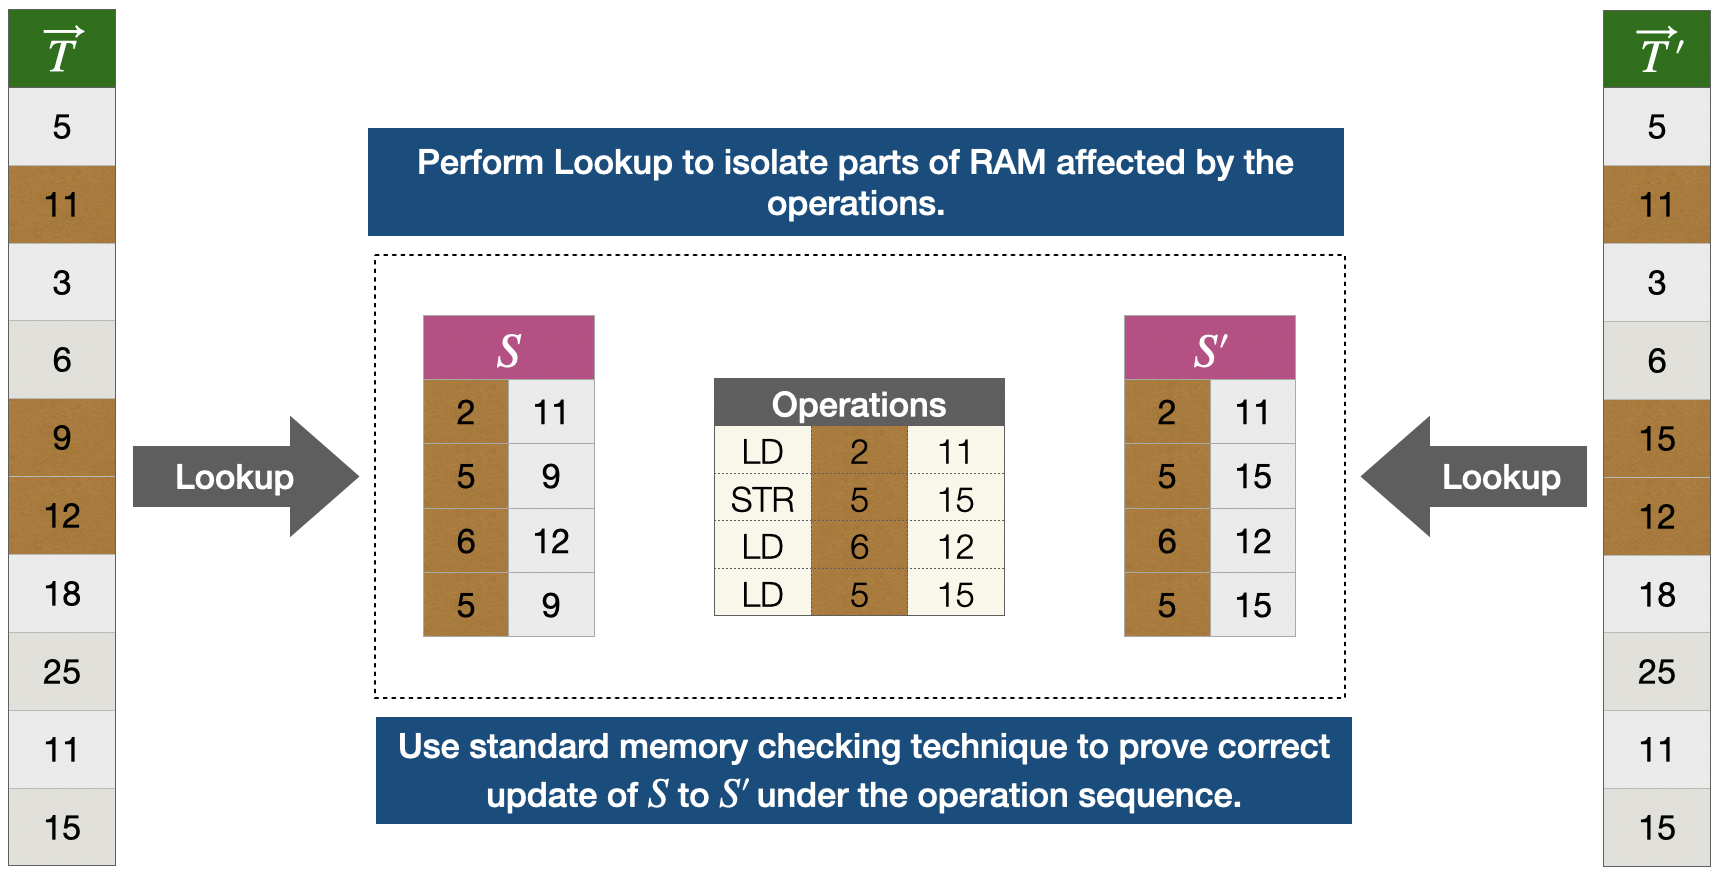
\includegraphics[width=\textwidth]{example-lookup}
\caption{Isolating subtables using lookup argument}
\label{fig:subtable-consistency}
\end{subfigure}
\begin{subfigure}{0.4\textwidth}
\centering
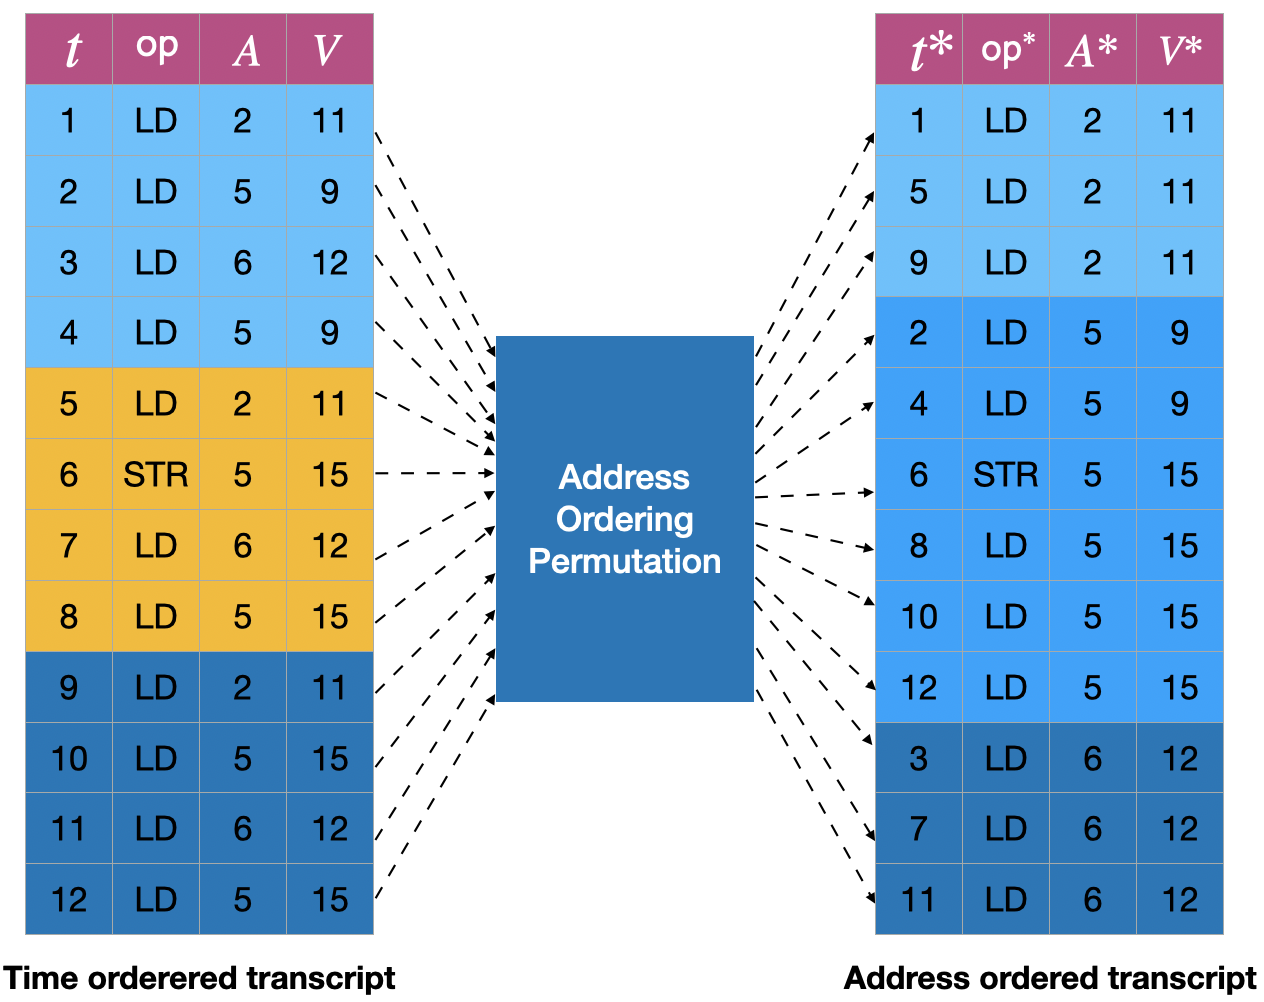
\includegraphics[height=0.3\textheight]{Address-ordered}
\caption{Checking memory consistency using address ordering}
\label{fig:permuted-transcripts}
\end{subfigure}
\end{figure}
\end{comment}



%
    \tikzset{
        table/.style={
            matrix of nodes,
            row sep=-\pgflinewidth,
            column sep=-\pgflinewidth,
            nodes={
                rectangle,
                draw=black,
                align=center
            },
            minimum height=1.5em,
            text depth=0.5ex,
            text height=1.5ex,
            nodes in empty cells,
%%
            every even row/.style={
                nodes={fill=gray!20}
            },
            column 1/.style={
                nodes={text width=2em}
            },
            row 1/.style={
                nodes={
                    fill=white,
                    text=black,
                    font=\bfseries
                },
            }
        }
    }

    \tikzset{
        MyArrow/.style={
            single arrow, draw=black, minimum width=10mm, minimum height=30mm, inner sep=0mm, single arrow head extend=1mm, double arrow head extend=1mm
        }
    }

    \begin{figure}[t]
        \centering
        %\subcaptionbox{Lookup to get sub-tables \label{fig:lookup}}[\textwidth]{
        \resizebox{0.8\textwidth}{0.3\textheight}{
        \begin{tikzpicture}
            %\draw[step=1.0,black,thin] (-5,-5) grid (5,5);
        \matrix (initial) [table,text width=2em, width=2cm] at (-5,1)
        {
            Idx & Val\\
            1  & 10 \\
            2  & 20 \\
            3  & 15 \\
            4  & 25 \\
            5  & 40 \\
            6 & 50 \\
            7 & 60 \\
        };

        \matrix (ops1) [table,text width=2em, width=2cm] at (0,0)
            {
            Op & Idx & Val \\
            \store  & 7 & 40 \\
            \load  & 1 & 10 \\
            \store & 3 & 20 \\
            \load  & 3 & 20 \\
        };


        \matrix (final) [table,text width=2em, width=2cm] at (5,1)
            {
            Idx & Val\\
            1  & 10 \\
            2  & 20 \\
            3  & 20 \\
            4  & 25 \\
            5  & 40 \\
            6 & 50 \\
            7 & 40 \\
        };


        % -------------------------------- Subtables ------------------------------------- %
        \matrix (stinitial) [table,text width=2em, width=2cm] at (-5,-5)
            {
            Idx & Val\\
            7 & 60 \\
            1 & 10 \\
            3 & 15 \\
            3 & 15 \\
        };

        \matrix (ops2) [table,text width=2em, width=2cm] at (0,-5)
            {
            Op & Idx & Val \\
            \store  & 7 & 40 \\
            \load  & 1 & 10 \\
            \store & 3 & 20 \\
            \load  & 3 & 20 \\
        };


        \matrix (stfinal) [table,text width=2em, width=2cm] at (5,-5)
            {
            Idx & Val\\
            7 & 40 \\
            1 & 10 \\
            3 & 20 \\
            3 & 20 \\
        };

            \draw (-5,3.6) node[above]  {\bf RAM $\vecT_0$};
            \draw (0, 1.6) node[above] {\bf Operations};
            \draw (5,3.6) node[above] {\bf RAM $\vecT_1$};
            \draw (-5, -3.4) node[above] {\bf $\vec{t}_0$};
            \draw (5, -3.4) node[above] {\bf $\vec{t}_1$};

            % lookup arrows
            \draw [-Latex, thick] (-4.25,-1.75) -- (-4.25,-3.25);
            \draw [-Latex, thick] (4.25, -1.75) -- (4.25, -3.25);
            \draw [fill=grey!30!white] (-2,-2) rectangle (2, -3) node[midway] {Lookup on indices 7,1,3,3};

            \draw (-2, -2.5) -- (-4.25, -2.5) (2, -2.5) -- (4.25, -2.5);
            \draw [-Latex, dashed] (-4, 0) -- (-1.6,0);
            \draw [-Latex, dashed] (1.6,0) -- (4,0);
            \draw [-Latex, dashed] (-4, -5) -- (-1.6,-5);
            \draw [-Latex, dashed] (1.6,-5) -- (4,-5);
        \end{tikzpicture}
        }
        \caption{Using lookup arguments to reduce the consistency check between large RAMs $\vecT_0$
        and $\vecT_1$ to that between small tables $\vec{t}_0$ and $\vec{t}_1$. It is seperately shown that RAMs $\vecT_0$ and
        $\vecT_1$ have identical values outside the involved indices. Figure ~\ref{fig:subtable-consistency} illustrates address
        ordered transcript to check consistency of $\vec{t}_0$ and $\vec{t}_1$.}
        \label{fig:subtable-lookup}
        \end{figure}

        \begin{figure}[htbp]
            \centering
            \resizebox{0.8\textwidth}{0.4\textheight}{
        \begin{tikzpicture}
        % ------------------------------------------------------------------------------------------- %
            %\draw[step=1.0,black,thin] (-5,-5) grid (5,5);
        \matrix (trts) [table,text width=2em] at (-4,0)
            {
            Ts & Op & Idx & Val\\
            1 & \store & 7 & 60 \\
            2 & \store & 1 & 10 \\
            3 & \store & 3 & 15 \\
            4 & \store & 3 & 15 \\
            5 & \store  & 7 & 40 \\
            6 & \load  & 1 & 10 \\
            7 & \store & 3 & 20 \\
            8 & \load  & 3 & 20 \\
            9 & \load & 7 & 40 \\
            10 & \load & 1 & 10 \\
            11 & \load & 3 & 20 \\
            12 & \load & 3 & 20 \\
        };

        \matrix (trts) [table,text width=2em, width=2cm] at (4,0)
            {
            Ts & Op & Idx & Val\\
            2 & \store & 1 & 10 \\
            6 & \load & 1 & 10 \\
            10 & \load & 1 & 10 \\
            3 & \store & 3 & 15 \\
            4 & \store  & 3 & 15 \\
            7 & \store  & 3 & 20 \\
            8 & \load & 3 & 20 \\
            11 & \load  & 3 & 20 \\
            12 & \load & 3 & 20 \\
            1 & \store & 7 & 60 \\
            5 & \store & 7 & 40 \\
            9 & \load & 7 & 40 \\
        };

            \path (-2.1,0) -- (1.9, 0)  node[midway, MyArrow, text width=3cm, align=center] {Address-sorting permutation};
            \draw (-4, 4.3) node[above] {\bf \small Time ordered transcript ($\mathsf{tr}$)};
            \draw (4, 4.3) node[above] {\bf \small Address ordered transcript ($\mathsf{tr}^\ast$)};

        \end{tikzpicture}
            }
            \caption{Address ordered transcript for checking consistency of tables $\vec{t}_0$ and $\vec{t}_1$
                with respect to the operation sequence in Figure \ref{fig:subtable-lookup}. On the transcript
            $\mathsf{tr}^\ast$, one checks that the load instructions return the same value as the preceeding
            instruction if their indices are the same.}

        \label{fig:subtable-consistency}
    \end{figure}





\section{Related Work}\label{sec:rel-work}
	Efficient modeling of the RAM primitive is a widely studied problem in
verifiable computation (VC), due to its inherent usefulness in modeling several computations of interest.
Encapsulating RAM semantics in VC circuits is also challenging; since (i) arithmetic/boolean circuits do not
adequately model random access, and (ii) incorporating entire memory as gates in a circuit is prohibitive.

Several novel techniques have been proposed to work around the above limitations of circuit based representation
of RAM. Among them, Merkle tree-based accumulators to model the RAM state are popular
~\cite{EPRINT:BFRSBW13,compwithstate,C:BCTV14} as they can efficiently
prove updates to the state, without modeling the entire memory in the arithmetic circuit. Other
approaches based on {\em address ordered time-scripts} avoid the concrete costs of Merkle tree-based approaches
by letting the prover provide inputs and outputs of RAM operations in a non-deterministic manner, which
are then checked to satisfy consistency of {\em loads} and {\em stores}.
Several works such as \cite{NDSS:WSRBW15,USENIX:BCTV14,C:BCGTV13,SP:ZGKPP18} implement and improve variants
of the aforementioned approach. Most transcript-based realizations of RAM only consider it to be transient,
i.e, its state is useful only during the execution of a program, and do not consider {\em persistence} of the
RAM state across several executions. 

Another feature, which has only been considered in recent works
\cite{USENIX:OWWB20,CCS:CFHKKO22} is {\em batching}, where a verifiable update of RAM state is required
for a batch of $m$ updates, with $m$ being much smaller than the RAM size. While constructions using Merkle tree-based accumulators~(realized from collision-resistant hash functions) suffer from high concrete costs and poor
ability to batch proofs, those based on checking consistency using transcripts incur a linear overhead in the
size of the RAM.

\smallskip

\noindent{\bf Batching-Efficient RAM.} There have been recent efforts~\cite{USENIX:OWWB20,CCS:CFHKKO22} on batching-efficient
realization of the RAM primitive~(see Table~\ref{tab:rel-work} for a summary of these schemes and the associated efficiency parameters). This is a natural setting in applications of verifiable
computation, most notably in the context of blockchain {\em rollups}. Here, one is required
to show that a batch of $m$ transactions correctly updates the state of a table of account balances, which
is maintained off-chain by the rollup provider. Here the batch-size $m$ ranges from few hundreds to few
thousands, whereas the table itself could contain several million accounts.
Similar to prior work on batching-efficient RAMs~\cite{USENIX:OWWB20,CCS:CFHKKO22}, our work is also motivated
 by the problem of enabling more efficient rollup for tables, which are
naturally modeled as RAMs.

While the aforementioned works substantially mitigate disadvantages of both the
Merkle-tree based approaches and transcript-based approaches by using RSA accumulators to model the state,
they still incur large prover costs and memory requirements even for modest sized batches. The approaches
in~\cite{USENIX:OWWB20,CCS:CFHKKO22} encode complex modular arithmetic over RSA groups and {\em hash
to prime} functions as arithmetic circuits, which results in a fixed overhead of around $10$ million R1CS constraints
at batch sizes of $m=1000$ (this overhead is significantly larger for ~\cite{USENIX:OWWB20}). This is already prohibitive on a modest hardware. In addition, the witness computation for each update incurs cost
linear in the size of accumulated set. The prior works~\cite{USENIX:OWWB20,CCS:CFHKKO22} seek to mitigate this through pre-computation and
parallel/distributed processing. However, the issue of maintaining pre-computed parameters in sync with dynamic accumulator state has not been adequately addressed in~\cite{USENIX:OWWB20,CCS:CFHKKO22}. For example, in RSA-based accumulators, generating $O(N)$ non-membership witnesses straightforwardly requires $O(N^2)$ time; however, these witnesses become stale once the accumulator state changes, and hence cannot be used as-is for subsequent update proofs. 

Our approach considers both the cost of online proof generation as well as the offline cost of maintaining pre-computed parameters. In addition, our solution is almost ``circuit-free''. Our entire RAM operation is modeled as a polynomial protocol, which is readily transformed into an argument of
knowledge using a polynomial commitment scheme. In an application of our primitive to rollups, the only part of the statement 
that would need to be expressed as a circuit is the verification of digital signatures on transactions~(which is around $500$ constraints per verification for EDDSA signatures). By suitably balancing the online and offline costs, we can prove a batch of $1000$ updates on a RAM of size $1$ million in an average of $90$ seconds on a commodity laptop with a single-threaded implementation. Our performance can be substantially improved using a parallel implementation. See Sections~\ref{sec:tech-overview} and~\ref{sec:experiments}  for more detailed discussions on the efficiency of our scheme. 

%Combining our novel update protocol with highly efficient
%lookup arguments such as~\cite{EPRINT:EagFioGab22}, our online proof generation can prove around $0.5$ million
%updates at an average of just $120$ seconds per batch of $1000$ updates on a commodity laptop. Even
%this performance is under worst-case assumption that each update is to a different position in the table.
%The expensive offline computation, mainly consisting of highly parallelized FFTs over groups requires around $3$ hours for a
%table of size 1 million, with a single-threaded implementation. Clearly, with more potent hardware and
%parallelization, one can process a table of size upto $10$ million in a few hours. 
%Our approach is also in the updatable SRS setting in constrast to trusted setup required for RSA parameter generation. We
%compare our work with the prior approaches more elaborately in Section ~\ref{sec:experiments}.


\smallskip

\begin{table*}[tb!]
	\begin{tabular}{|llll|}
		\hline
		\multicolumn{1}{|l|}{\textbf{Scheme}} & \multicolumn{1}{l|}{\textbf{Proof Size}} & \multicolumn{1}{l|}{\textbf{Prover Work}} & \textbf{Verifier Work} \\ \hline
		\rowcolor{gray}
		\multicolumn{4}{|c|}{\textcolor{white}{Lookup Arguments for Static Tables}} \\ \hline
		\multicolumn{1}{|l|}{Plookup \cite{EPRINT:GabWil20}} & \multicolumn{1}{l|}{$5 \Gone, ~9\F$} & \multicolumn{1}{l|}{$O(N) \,\Gone$, $O(N\log N) \,\F$} & $2P$ \\ \hline
		\multicolumn{1}{|l|}{Halo2 \cite{EPRINT:BowGriHop19,Halo2}} & \multicolumn{1}{l|}{$6 \Gone, ~5\F$} & \multicolumn{1}{l|}{$O(N) \,\Gone$, $O(N\log N) \,\F$} & $2P$ \\ \hline
		\multicolumn{1}{|l|}{Caulk \cite{CCS:ZBKMNS22}} & \multicolumn{1}{l|}{$14 \Gone, ~1 \Gtwo, ~4\F$} & \multicolumn{1}{l|}{$15m \,\Gone$, $O(m^2+m\log N) \,\F$} & $4P$ \\ \hline
		\multicolumn{1}{|l|}{Caulk+ \cite{EPRINT:PosKat22}} & \multicolumn{1}{l|}{$7 \Gone, ~1 \Gtwo, ~2\F$} & \multicolumn{1}{l|}{$8m \,\Gone$, $O(m^2) \,\F$} & $3P$ \\ \hline
		\multicolumn{1}{|l|}{Flookup \cite{EPRINT:GabKho22}} & \multicolumn{1}{l|}{$7 \Gone, ~1 \Gtwo, ~2\F$} & \multicolumn{1}{l|}{$O(m) \,\G$, $O(m \log^2 m) \,\F$} & $3P$ \\ \hline
		\multicolumn{1}{|l|}{Baloo \cite{EPRINT:ZGKMR22}} & \multicolumn{1}{l|}{$12 \Gone, ~1 \Gtwo, ~4\F$} & \multicolumn{1}{l|}{$14m \,\G$, $O(m \log^2 m) \,\F$} & $5P$ \\ \hline
		\multicolumn{1}{|l|}{CQ \cite{EPRINT:EagFioGab22}} & \multicolumn{1}{l|}{$8 \Gone, ~3\F$} & \multicolumn{1}{l|}{$8m \,\Gone$, $O(m \log m) \,\F$} & $5P$ \\ \hline
		\multicolumn{1}{|l|}{CQ+ \cite{PKC:CFFLL24}} & \multicolumn{1}{l|}{$7 \Gone, ~1\F$} & \multicolumn{1}{l|}{$8m \,\Gone$, $O(m \log m) \,\F$} & $5P$ \\ \hline
		\multicolumn{1}{|l|}{Locq \cite{PKC:ZSG24}} & \multicolumn{1}{l|}{$4 \Gone, ~1 \Gtwo$} & \multicolumn{1}{l|}{$6m \,\Gone$, $m \,\Gtwo$, $O(m \log m) \,\F$} & $4P$ \\ \hline
		\multicolumn{1}{|l|}{Lasso \cite{lasso}} & \multicolumn{1}{l|}{$O(1) \,\G, ~O(\log m) \,\F$} & \multicolumn{1}{l|}{$o(cm+cN^{1/c}) \,\Gone$, $O(cm) \F$} & $O(\log m) \,\F$, $O(1) \,\G$ \\ \hline
		\rowcolor{gray}
		\multicolumn{4}{|c|}{\textcolor{white}{Lookup Arguments for Updatable Tables/Batching-Efficient RAM}} \\ \hline
		\multicolumn{1}{|l|}{OWWB20~\cite{USENIX:OWWB20}} & \multicolumn{1}{l|}{} & \multicolumn{1}{l|}{} & \\ \hline
		\multicolumn{1}{|l|}{B-INS-ARISA~\cite{CCS:CFHKKO22}} & \multicolumn{1}{l|}{} & \multicolumn{1}{l|}{} &  \\ \hline
		\multicolumn{1}{|l|}{\begin{tabular}[c]{@{}l@{}}Our work\\ (using CQ)\end{tabular}} & \multicolumn{1}{l|}{$8 \Gone, ~3\F$} & \multicolumn{1}{l|}{$8m \,\G$, $O(m \log m) \,\F$} & $5P$ \\ \hline
	\end{tabular}
	\caption{Comparison with state-of-the-art lookup arguments. For comparison against Lasso (reported considering their polynomial commitment scheme Sona and structured tables), $c$ denotes an arbitrary positive integer. Note that our lookup argument inherits the complexity of the underlying lookup argument used in a black-box manner and can be instantiated with any of the non-updatable lookup arguments.}
	\label{tab:rel-work}
\end{table*}

\noindent{\bf Lookup Arguments.} There are several recently proposed constructions of lookup arguments which enable proving that a vector of size $m$ is a sub-vector of a larger~(predetermined) vector of size $N$~(see Table~\ref{tab:rel-work} for a summary of these schemes and the associated efficiency parameters). Of these, the very initial schemes~\cite{EPRINT:BowGriHop19,EPRINT:GabWil20,Halo2} incur proving costs linear in $N$. Starting with Caulk~\cite{CCS:ZBKMNS22}, many lookup arguments were proposed with proving costs that are (largely) independent of $N$. Broadly, these schemes can be divided into categories based on how they achieve proving costs independent of $N$. The lookup arguments in the first category~\cite{CCS:ZBKMNS22,EPRINT:PosKat22,EPRINT:GabKho22,EPRINT:EagFioGab22,EPRINT:ZGKMR22,PKC:CFFLL24,PKC:ZSG24} use polynomial protocols in conjunction with the $\kzg$ polynomial commitment scheme, where the lookup efficiency relies crucially on \textit{pre-computed} $\kzg$ opening proofs for the polynomial encoding the predetermined $N$-sized vector. We point out that na\"ively adapting these lookup arguments for updatable tables/RAM is challenging since even small updates to the table require re-computing all of the opening proofs, which is prohibitively expensive~(requires $\wt{O}(N)$ computation). To overcome the ``rigidity'' inherent to these schemes, we propose a new method of constructing lookup arguments which allows re-using the pre-computed opening proofs across several batch updates, thus avoiding the need for re-computing after each batch~(see Sections~\ref{sec:tech-overview} and~\ref{sec:update-protocol} for more details). 


%Caulk~\cite{CCS:ZBKMNS22} provides with lookup arguments where a vector of size $m$ is proved to be a subvector of a large vector of size $N$, while maintaining privacy regarding the positions of the subvector (called \emph{position-hiding linkability}) where the prover complexity is $O(m^2+m\log N)$ with $O(N\log N)$ preprocessing and $O(N)$ storage. Caulk+~\cite{EPRINT:PosKat22} improves over Caulk to $O(m^2)$ prover complexity by removing the dependency on the size of the large vector $N$, and CQ~\cite{EPRINT:EagFioGab22}, using the ``logarithmic derivative based lookup" of \cite{Eag22,Hab22}, further improves it to $O(m\log m)$, while retaining the same $O(N\log N)$ preprocessing. Additional lookup arguments, namely cq+, cq++, zkcq+~\cite{pkc-lookup-mat} and locq~\cite{PKC:ZSG24} provides further improvements over CQ.
%However, we aim to provide committed index lookup arguments that can `link' a set of indices in the vector of size $N$ to the `claimed' subvector of size $m$, that helps in ensuring that we can always `lookup' relevant indices from a committed vector. Additionally, note that the prior works provides lookup arguments for `static' tables, i.e. any `updates' to the large table requires $O(N\log N)$ recomputation each time in the prior works. Our work ensures a batching friendly preprocessing can be done whenever there are incremental changes to the vector of size $N$, and avoid performing the $O(N\log N)$ recomputation per update. This modification extends to the other works as well. We also present techniques to extend lookup argument \cite{EPRINT:EagFioGab22}, which uses homomorphic commitments, to provide a committed index lookup argument.

\smallskip

\noindent{\bf Lasso.} The second category of lookup arguments is exemplified by the recently proposed Lasso scheme~\cite{lasso,jolt}, which enables efficient lookups for tables with a decomposable structure. Informally, a table $\vecT:\{0,1\}^n\to \{0,1\}^k$ is said to have a decomposable structure if there exists a decomposition of the table $T$ into $c$ sub-tables $\vecT_1,\ldots,\vecT_c:\{0,1\}^{n/c} \to\{0,1\}^\ell$ and a very efficiently computable function $f$ such that for $x = x_1\|\ldots\|x_c$ where $x_i \in \{0,1\}^{n/c}$, we have
\[\vecT[x] = f(\vecT_1(x_1),\ldots,\vecT_c(x_c))\]
A simple example of such a function is a bit-wise AND~(we refer to~\cite{lasso,jolt} for a more detailed exposition). Lasso crucially leverages this decomposability of the table to reduce a lookup into a table of size $N=2^n$ into $c$ lookups, each into a table of size $N^{1/c}$. While this strategy works elegantly for tables with special structure, it is not compatible with arbitrary tables/updates, which is the focus of our work~(in particular, in applications such as rollups, we need the ability to handle updates to arbitrary tables).

To summarize, existing lookup arguments achieve efficiency either by leveraging table-specific pre-computations or specially structured tables, both of which do not na\"ively extend to arbitrary dynamic tables. We focus on handling batch updates for arbitrary tables, and our techniques can be viewed as enabling the utility of table-specific parameters even \textit{across batch updates}.    

%However, 
%
%consider a table $T$
%
%In the literature, to provide sublinear lookups for large tables, either one cleverly uses preprocessing to ensure optimal online cost or one leverages a predefined structure in the tables in consideration.
%Lasso~\cite{lasso} gives a new family of lookup arguments for the second category, where the prover's cost only grows with table entries that are accessed by the lookup operations, for tables that are structured. Lasso provides efficient lookups by leveraging a predefined relation between the large table and the `looked-up' small table, where the large table has tensor-structure and is efficiently `decomposable'. This structure  helps to reduce number of elements which need to be committed, in turn reducing the prover time as well.
%On the contrary, our work applies to tables without any structure (as is the case with rollup application), and additionally we can handle \emph{updatable} %\chaya{agree on spelling of updatable throughout} 
%tables. 


%Note that lasso crucially leverages the tensor-structure of static tables, and uses techniques that are inherently incompatible with arbitrary updates which is essential for handling arbitrary state updates in our considered application and the prover complexity would still be linear in the large table for arbitrary tables which lacks the tensor-structure. 
%Therefore, to support arbitrary updates, our work relies on optimally using and updating the pre-computed parameters instead.
%Lasso also defines a committed index lookup relation like us and gives a reduction between indexed and unindexed lookups (subvector relation); however, their reduction needs an upper bound on the elements of the table. We provide a different reduction without this restriction. 
%A recent work called Jolt~\cite{jolt} expresses all constraints of a computation as lookups by creating a lookup table that contains the entire evaluation table of each instruction $f$ in an instruction set.
%This approach of using table lookups requires memory checking arguments as well. However Jolt uses lookup arguments to \emph{model} CPU operations, whereas our work uses lookup arguments to reduce the size of memory in memory-checking methods. \chaya{could add a line here or in conclusion that our techniques could be used to improve Jolt's mem consistency approach.}






\section{Preliminaries}\label{sec:prelims}
    
Throughout the paper, we assume a bilinear group generator $\bg$ which on input $\lambda$ outputs
parameters for the protocols. Specifically $\bg(1^\secp)$ outputs $(\F,\Gone,\Gtwo,\GT, e, g_1, g_2,g_t)$
where:
\begin{itemize}[leftmargin=2em, label=-]
	\item $\F=\Fp$ is a prime field of super-polynomial size in $\lambda$, with $p=\lambda^{\omega(1)}$.
	\item $\Gone,\Gtwo$ and $\GT$ are groups of order $p$, and $e$ is an efficiently computable non-degenerate
	pairing $e:\Gone\times \Gtwo\rightarrow \GT$.
	\item Generators $g_1,g_2$ are uniformly chosen from $\Gone$ and $\Gtwo$ respectively and $g_t=e(g_1,g_2)$.
\end{itemize}
We write groups $\Gone$ and $\Gtwo$ additively, and use the shorthand notation $\gone{x}$ and $\gtwo{x}$
to denote group elements $x\cdot g_1$ and $x\cdot g_2$ respectively for $x\in \F$. We will implicity assume
that all the setup algorithms for the protocols invoke $\bg$ to generate descriptions of groups and fields
over which the protocol is instantiated. We will use the notation
$[n]$ to denote the set of integers $\{1,\ldots,n\}$.

\noindent{\bf Security Model}: We describe public-coin interactive protocols, involving a prover and a verifier,
where both the parties have access to a structured reference string (SRS). The SRS in our protocol consists of
encodings of monomials of the form $\left\{\gone{x^i}\}_{a\leq i\leq b}$, $\left\{\gtwo{x^i}\}_{c\leq i\leq d}$
for $x$ chosen uniformly from $\F$ and $a,b,c,d$ are bounded by some polynomial in $\lambda$. It then follows
from ~\cite{EPRINT:BowGabMie17} that such an SRS can be generated using a universal and updatable setup requiring
only one honest participant. In practice, this gives us a far superior security model to the one requiring a fully
trusted setup. We use $\srs = (\srs_1,\srs_2)$ to denote the structured reference string of the above form. We say
that the $\srs$ has degree $Q$ if all the elements of $\srs_i$, $i=1,2$ are of the form $[f(x)]_i$ for a
polynomial $f\in \F_{<Q}[X]$.\smallskip


\noindent{\bf Algebraic Group Model}: We analyse our protocols in the Algebraic Group Model (AGM) introduced
in ~\cite{C:FucKilLos18}. We consider {\em algebraic adversaries} $\Adv$, which in our SRS-based protocol means
an efficient algorithm satisfying the following:
\begin{itemize}[leftmargin=1em]
	\item For $i\in \{1,2\}$, whenever $\Adv$ outputs an element $A\in \G_i$, it also outputs a vector $\vec{v}$
	over $\F$ such that $A=\langle \vec{v},\srs_i\rangle$.
\end{itemize}
Algebraic group model is a useful framework for obtaining succinct arguments of knowledge (SNARKs) from interactive
protocols described as {\em polynomial protocols} ~\cite{Gabizon2019PLONKPO}. Informally, the prover's messages in
a polynomial protocol are low degree polynomials, and the verifier accepts or rejects by checking certain identities
over polynomials output by the prover and possibly public polynomials known to the verifier. A polynomial protocol can
be compiled into a succinct argument of knowledge by using an extractable polynomial commitment scheme, which allows a
prover to send commitments to polynomials, and later send evaluation proofs for the same to enable the verifier to probabilistically
check polynomial identities at random points of $\F$. We refer the reader to ~\cite[Section 4.2]{Gabizon2019PLONKPO} for details
on polynomial protocols and their compilation to SNARKs in the algebraic group model.

\subsection{KZG Commitment Scheme}
\label{sec:KZG}
We use the $\kzg$ commitment scheme introduced in ~\cite{AC:KatZavGol10} which satisfies succinctness, completeness and knowledge-soundness (extractability)
in the algebraic group model, while additionally featuring a universal and updatable setup. We denote the $\kzg$ scheme by the tuple
of $\ppt$ algorithms $(\KZGsetup$,$\KZGcommit$, $\KZGopen$, $\KZGverify)$ as defined below.
%We then establish the isomorphism of the KZG polynomial commitment scheme as a vector commitment scheme.
\begin{definition}[KZG Polynomial Commitment Scheme]
	Let $(\F,\Gone,\Gtwo,\GT, e, g_1, g_2, g_t)$ be output of bilinear group generator $\bg(1^\secp)$ for security parameter $\secp$.
	The KZG polynomial commitment scheme is defined as follows:
	\begin{itemize}[leftmargin=1em]
		\item $\KZGsetup$ on input $(1^\secp,d)$, where $d$ is the degree bound, outputs
		$\srs = \{\eltone{\tau},\ldots,\eltone{\tau^d}\}$ ,$\{\elttwo{\tau},\ldots,\elttwo{\tau^d}\}$.
		\item $\KZGcommit$ on input $(\srs,p(X))$, where $p(X) \in \F_{\leq d}[X]$, outputs $C=\eltone{p(\tau)}$
		\item $\KZGopen$ on input $(\srs,p(X),\alpha)$, where $p(X) \in \F_{\leq d}[X]$ and $\alpha\in \F$, outputs $(v, \pi)$ such that $v=p(\alpha)$ and $\pi=\eltone{q(\tau)}$, for
		\[ q(X)=\frac{p(X)-p(\alpha)}{X-\alpha} \]
		\item $\KZGverify$ on input $(\srs,C,\alpha,v,\pi)$, outputs $1$ if the following equation holds, and $0$ otherwise.
		\[ e(C-v, \elttwo{\tau}) = e(\pi, \elttwo{\tau-\alpha}) \]
	\end{itemize}
\end{definition}

We also assume (w.l.o.g) analogues of $\KZGcommit$, $\KZGopen$ and $\KZGverify$ defined over the group $\Gtwo$.
We shall use the (non-standard) notation $[p(X)]_i$ to denote $[p(\tau)]_i$ for $i\in \{1,2\}$.
This allows us a convenient shorthand for referring to ``commitment of the polynomial $p(X)$'' in group $\G_i$.
Our protocols also use batched KZG proofs to show that polynomial $p(X)$ satisfies $p(\alpha_i)=v_i$ for $i\in [n]$. Let
$\vec{\alpha}=(\alpha_1,\ldots,\alpha_n)$
denote the vector of evaluation points and $\vec{v}=(v_1,\ldots,v_n)$ denote the vector of claimed evaluations. Then the batched
version of $\KZGopen$ is described as follows:
\begin{itemize}[leftmargin=1em]
	\item $\KZGopen$ on input $(\srs,p(X),\vec{\alpha})$, where $p(X) \in \F_{\leq d}[X]$ and $\vec{\alpha}\in\F^n$,
	outputs $(\vec{v}, \pi)$ with $\vec{v}\in \F^n$ such that $v_i=p(\alpha_i)$ and $\pi=\eltone{q(\tau)}$ where
	\[ q(X)=\frac{p(X)-r(X)}{a(X)} \]
	In the above, $a(X)=(X-\alpha_1)\cdots(X-\alpha_n)$, while $q(X)$ and $r(X)$ are the quotient and remainder polynomials when
	 $p(X)$ is divided by $a(X)$.
	%Note that the polynomials $a(X)$ and $r(X)$ can be computed by the verifier since $\{\alpha_i,v_i\}_{i\in [n]}$ are known and
	%$a(X)=(X-\alpha_1)\cdots(X-\alpha_n)$ and $r(\alpha_i)=v_i$ for all $i\in [n]$ such that $0\leq \deg(r(X)) \leq n$.
	\item $\KZGverify$ on input $(\srs,C,\vec{\alpha},\vec{v},\pi)$, outputs $1$ if the following equations holds, and $0$ otherwise.
	\begin{align*}
		e(C-\eltone{r(\tau)}, \elttwo{\tau}) &= e(\pi, \elttwo{a(\tau)})
	\end{align*}
	Here, the verifier interpolates the polynomial $r(X)\in \F_{<n}[X]$ such that $r(\alpha_i)=v_i$.
\end{itemize}

%\begin{definition}[KZG Polynomial Commitment Scheme \textcolor{red}{degree check included}]
%    Let $(p,\Gone,\Gtwo,\GT, e, \eltone{1},\elttwo{1})$ be a bilinear group. The KZG polynomial commitment scheme is defined as follows: 
%    \begin{itemize}
%	        \item $\KZGsetup$ on input $(1^\lambda,d)$, where $\lambda$ is the security parameter and $d$ is the degree bound, outputs $\srs = \{ \eltone{\tau},\ldots,\eltone{\tau^d},\elttwo{\tau},\ldots,\elttwo{\tau^d}\}$
%	        \item $\KZGcommit$ on input $(\srs,p(X))$, where $p(X) \in \F_{\leq d}[X]$, outputs $C=\eltone{p(X)}:=\eltone{p(\tau)}$
%	        \item $\KZGopen$ on input $(\srs,p(X),\alpha)$, where $p(X) \in \F_{\leq d}[X]$ and $\alpha\in \F$, outputs $(v, \pi)$ such that $v=p(\alpha)$ and $\pi=\Comtwo{q(X)}:=\elttwo{q(\tau)}$, for
%	        \[ q(X)=\frac{p(X)-p(\alpha)}{X-\alpha} \]
%	        \item $\KZGverify$ on input $(\srs,C,\deg,\alpha,v,\pi)$, outputs $1$ if the following equation holds, and $0$ otherwise.
%	        \[ e(C-v, \elttwo{\tau}) = e(\pi, \elttwo{\tau-\alpha}) \]
%	        { \color{teal} \moumita{var 3.}
%		        Degree check has not been added. With degree check, $\pi$ is modified with
%		        \[ q(X)=X^{d-\deg(p(X))+2}\frac{p(X)-p(\alpha)}{X-\alpha} \]
%		        and the verification equation if modified as 
%		        \[ e(C-v, \elttwo{\tau}^{d-\deg+2}) = e(\pi, \elttwo{\tau-\alpha}) \]
%		        } %stays unchanged from var 1
%	    \end{itemize}
%\end{definition}
\nitin{Defer the commitment to vectors to where we need it}
\begin{comment}
\paragraph{Vector Commitment Scheme.} We note that there is a natural isomorphism between the set of vectors of length $n$ and polynomials of degree $n-1$, where any vector $\abf=(a_1,\ldots,a_n) \in \F^n$ has a natural equivalent representation as a polynomial $a(X)=a_1\lambda_1(X)+\ldots,a_n\lambda_n(X)$, where $\{\lambda_i(X)\}_{i\in [n]}$ is basis of $\F_{\leq n-1}[X]$. Hence, when we use the KZG polynomial commitment scheme for a vector $\abf=(a_1,\ldots,a_n) \in \F^n$, we can output the commitment as $\KZGcommit(\srs,a(X))$, where $a(X)=a_1\lambda_1(X)+\ldots,a_n\lambda_n(X)$.


Now, for vectors of length $n$, we consider the basis $\{\lambda_i(X)\}$ to be the langrange basis with respect to the set consisting of $n^{th}$ roots of unity $\doubleH=\{\omega,\ldots,\omega^n\}$. The lagrange basis helps us use the property that, for some $i\in [n]$ and a value $\alpha$, $a(\omega^i)=a_i=\alpha$ if and only if there exists a polynomial $W(X)$ such that $W(X)=\frac{a(X)-\alpha}{X-\omega^i}$. 
\end{comment}
%Throughout the draft, for $\abf\in \F^n$, we use $\Comone{.}$ to denote $\KZGcommit(\srs,\abf)$ for vectors of length $n$, using the langrange polynomial basis $\{\lambda_i(X)\}$, with respect to the $n^{th}$ root of unity $\omega$, and for $\bbf \in \F^m$, we use $\Comtwo{.}$ to denote $\KZGcommit(\srs,\bbf)$ for vectors of length $m$, using the langrange polynomial basis $\{\mu_i(X)\}$, with respect to the $m^{th}$ root of unity $\nu$.

	\section{Technical Overview}\label{sec:tech-overview}
As we have alluded to earlier, existing memory-checking based techniques to model RAM computations incur a cost
that is linear in the size of the RAM. We are interested in the setting where the number of operations whose
execution is to be verified is much smaller than the size of the RAM. Thus, our goal is to achieve prover complexity
which is {\em sublinear} in the size of the RAM. Before we proceed, we establish a
working definition of RAM for the rest of the paper. Informally, a RAM maps indices (addresses) to values, where
we assume that values come from a finite field $\F$, while indices come from a subset $\setind$ of $\F$. For us,
$\setind$ will generally be the set $\{1,\ldots,k\}$ for some integer $k$ (which may be different from size of
the RAM $n$). Finally, for an index, there should be at most one value in the RAM, i.e., the association is unambiguous.
The formal definition of RAM is as follows:
\begin{definition}[RAM]\label{defn:RAM}
Given $n\in \N$, finite field $\F$ and a set $\mathcal{I}\subseteq \F$, a RAM of size $n$ over indices $\mathcal{I}$
is a tuple $\vecT=(\vec{a},\vec{v})\in \mathcal{I}^n\times \F^n$ such that $\forall\, i,j\in [n]$  $v_i=v_j$ whenever $a_i=a_j$.
We think of $\vecT$ as a table with vectors $\vec{a}$ and $\vec{v}$ denoting its columns. The set of all such
tables will be denoted by $\RAM{I}{n}$.
    %\begin{align*}
    %        T[\,a\,] = \begin{cases}
    %                   v \text{ if } \, \exists i\in [n] \text{ s.t. } (a,v) = (a_i,v_i), \\
    %                  \bot \text{ otherwise }
    %                \end{cases}
    %\end{align*}
\end{definition}
For a table $\vecT=(\vec{a},\vec{v})\in \RAM{I}{n}$, we refer to tuples $(a_i,v_i)$, $i\in [n]$ as records of the table $\vecT$.
We use the access notation $v=\vecT[a]$ to mean that $(a,v)$ is a record of $\vecT$ (note there can be multiple such records
according to our definition). When we consider RAMs where the first column~(of indices) is of the form $\vec{I}_n=(1,2,\ldots,n)$, we simply 
denote such RAMs by $\vecT\in\F^n$.
%When we refer to a vector $\vecT\in \F^n$ as a RAM, we implicitly
%assume the first column of the RAM $\vecT$ to be $\vec{I}_n=(1,2,\ldots,n)$. 
%$T=(\vec{I}_n,\vecT)$ with $\vec{I}_n=(1,2,\ldots,n)$. In this case we have $T[i]=\vecT[i]$.
For a RAM $\vecT\in \RAM{I}{n}$, a RAM operation is a three tuple $(\op,a,v)$ with $\op\in \{0,1\}$,
$a\in \setind$ and $v\in \F$. An operation with $\op=0$ is called a {\em load} operation which denotes reading a value $v$
mapped to index $a$ in the RAM. Similarly, an operation with $\op=1$ is called a {\em store} operation,
which denotes associating the value $v$ with index $a$ in the RAM.
We use $\RAMOp{I}$ to denote the set of all RAM operations with index set $\setind$.

\begin{table*}[bt]
    \begin{tabular}{l|l|l|l|l}
        \hline
        {\bf Component  }                                                                                      & {\bf Protocol} & {\bf Prover Work}      & {\bf Verifier Work} & {\bf Communication}   \\ \hline
        Committed Sub-vector Lookup                                                                     & CQ ~\cite{EPRINT:EagFioGab22}      & $O(m \log m)\,\F$, $O(m)\,\Gone$      & $5P$            & $8\Gone$, $3\F$         \\ \hline
        Committed Index Lookup                                                                          & Fig ~\ref{fig:committed-index-lookup}    & $O(m \log m)\,F$, $O(m)\,\Gone$      & $5P$            & $8\Gone$, $3\F$         \\ \hline
        Localized Update in RAM                                                                                & Fig ~\ref{fig:a-identical}   & $O(m \log^2 m)\, \F$, $O(m)\,\Gone$      & $8P$            & $19\Gone$, $1\Gtwo$, $10\F$ \\ \hline
        Table Specific Preprocessing                                                                    & Fast KZG ~\cite{EPRINT:FeiKho23}      & $O(N \log N)\,\F,\G$      & -             & -               \\ \hline
        Lookup from Approximate Setup                                                                   & Sec ~\ref{sec:update-protocol}    & $O((m+\delta)\log^2(m+\delta))\,\F$, $O(m+\delta)\,\Gone$ & -             & -               \\ \hline
        Polynomial Protocol for RAM                                                                     & Fig ~\ref{fig:covering-protocol}   & $O(m \log m)\F,\, O(m)\G$      & $7P$            & $36\Gone$, $30\F$       \\ \hline
        %	Concatenation of transcripts                                                                    & Fig 8    & $O(m \log m)$      & 2P            & 4G1, 6F         \\ \hline
        %	Permutation of transcripts                                                                      & Fig 9    & $O(m \log m)$       & 2P            & 4G1, 5F         \\ \hline
        %	\begin{tabular}[c]{@{}l@{}}Memory consistency \& \\ address ordering of transcript\end{tabular} & Fig 7    & $O(m \log m)$       & 5P            & 20G1,19F        \\ \hline
        \rowcolor{lightgray}
        {Batching-Efficient RAM}                                                                          & {Fig  ~\ref{fig:complete-listing}}    & {$\widetilde{O}(\sqrt{mN})\,\F,\G$}            & ${9P}$            & {$65\Gone$, $1\Gtwo$, $43\F$}  \\ \hline
    \end{tabular}
    \caption{Asymptotic efficiency of the component protocols for our scheme. Here $N$ = size of the RAM, $m$ = number of operations
    , $\delta$ = Hamming distance of table for which pre-computed parameters are available from the current table.
    $P$ denotes a pairing evaluation. The performance corresponds to CQ based realization of batching-efficient
    RAM.}
    \label{tbl:efficiency-components}
    \vspace*{-5mm}
\end{table*}



\subsection{Batching-Efficient RAM: Blueprint}\label{subsec:batching-efficient-ram-blueprint}
We will use a vectors in $\F^N$ to denote the ``large'' RAMs, where index column is implicitly
assumed to be $(1,\ldots,N)$.
Let $\vecT,\vec{T'}\in \F^N$ denote the initial and final RAM states, and let $\vec{o}$ be
a sequence of $m$ operations ($m < N$) which updates $\vecT$ to $\vecT'$. Let $\vec{a}\in \F^m$ denote the vector
of RAM indices referenced by the operations in $\vec{o}$, i.e, $a_i$ is the index referenced by the $i^{th}$ operation.
To prove the transformation of $\vecT$ to $\vecT'$ via operation sequence $\vec{o}$, we proceed as follows:
\begin{itemize}[leftmargin=1em, label=-]
    \item We isolate sub-tables $S=(\vec{a},\vec{v})$ and $S'=(\vec{a},\vec{v'})$ of $\vecT$ and $\vecT'$ consisting of
    rows corresponding to indices in $\vec{a}$. This requires proving $\vec{v}=\vecT[\vec{a}]$ and $\vec{v'}=
    \vecT'[\vec{a}]$, which we show using {\em committed index lookup} argument discussed in Section ~\ref{subsec:committed-index-lookup}.

    \item On the isolated sub-tables $S$ and $S'$ of size $m$, we use the standard memory checking arguments (c.f. argument
    presented in Section \ref{sec:poly-proto-ram-app}) to prove that sequence $\vec{o}$ correctly updates $S$ to $S'$ with
    prover complexity of $\wt{O}(m)$.

    \item Finally, we show that the RAMs $\vecT$ and $\vecT'$ are identical outside indices in $\vec{a}$. We describe the protocol
    for proving the same in Section ~\ref{subsec:proximity-ram}.
\end{itemize}

\begin{figure}[htbp]
    \centering
    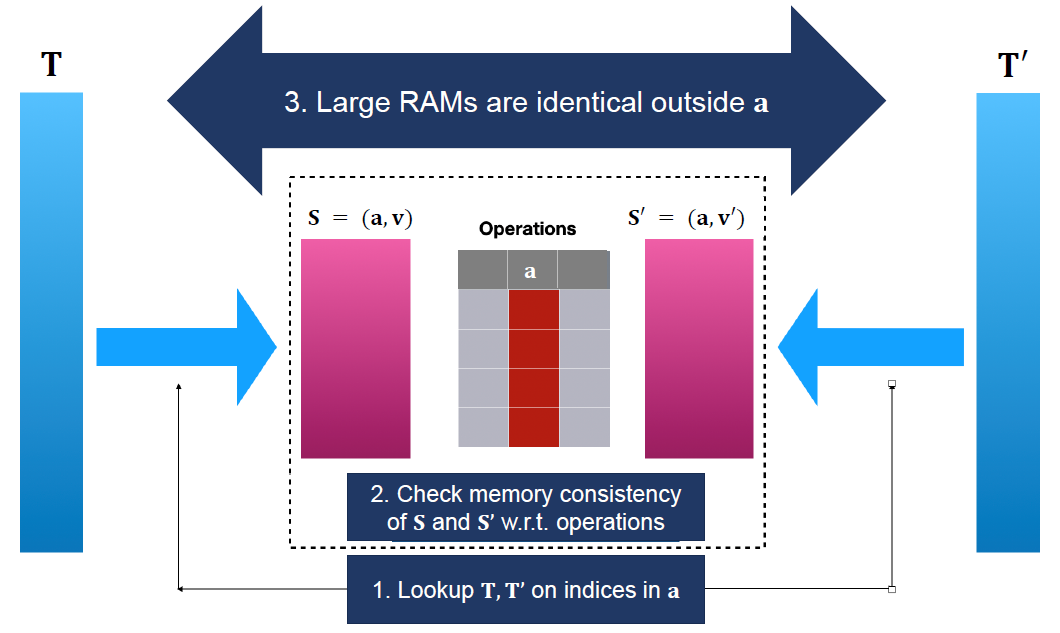
\includegraphics[width=0.49\textwidth]{RAM-Lookup}
    \caption{Illustrating different steps of sub-linear lookup protocol between large RAMs $\vecT$ and $\vecT'$.}
    \label{fig:blueprint}
\end{figure}

The blueprint for the above approach is illustrated in Figure ~\ref{fig:blueprint}.

\subsection{Batching-Efficient RAM: Components}\label{subsec:batching-efficient-ram-components}
We now elaborate on the key technical components in realizing the above blueprint.

\smallskip

\noindent{\bf Committed Index Lookup.} To limit the size of the RAM on which we use memory-checking techniques,
our first step is to isolate sub-tables of RAMs $\vecT$ and
$\vecT'$ corresponding to addresses which are involved in the operations.
This is achieved by looking up RAMs $\vecT$ and
$\vecT'$ at indices in the committed vector $\vec{a}$. We could leverage the recent work on efficient lookup
arguments to verifiably extract $m$ indices from a table of size $N$, in time dependent only on $m$.
However, there are two technical challenges here. First, the aforementioned lookup arguments only prove the sub-vector
relation, without linking the extracted vector to the indices in $\vec{a}$. This is easily solved, as there
is an efficient realization of a {\em committed index lookup} from a {\em committed sub-vector} argument,
where the commitment scheme is homomorphic. The details appear in Section ~\ref{subsec:committed-index-lookup},
with the complete protocol presented in Figure ~\ref{fig:committed-index-lookup}. The second challenge is much more
formidable: the efficiency of sub-vector arguments (and the committed index lookup argument derived from them)
depends on {\em expensive} table-specific pre-processing. This is acceptable when the table in question is
static, but is infeasible in our setting requiring updatable tables. This motivates our next technical
component.

\smallskip

\noindent{\bf Fast Lookup from Approximate Setup.} We build upon the rich body of work on polynomial protocols enabling efficient lookups from static tables~\cite{CCS:ZBKMNS22,EPRINT:PosKat22,EPRINT:ZGKMR22,EPRINT:EagFioGab22}, which rely on expensive table-dependent pre-computation
to optimise online proving performance. We make the first attempt towards breaking this rigid dependence.
Our key idea is to extend the utility of pre-computed
parameters for a table $\vecT$, to proving lookups from tables $\vecT'\neq \vecT$.
We show that for $\delta=\Delta(\vecT, \vecT')$,
an argument for $m$ lookups from $\vecT'$ incurs an additional prover overhead of $(m+\delta)\log^2(m+\delta)$ over the
lookup argument for static tables. We note that the overhead is {\em quasi}-linear in both $m$ and $\delta$.
Our competitive overhead rests on several innovative applications of algebraic
algorithms, which are summarised in Section ~\ref{subsec:comp-algebra-app}. We then leverage this ability to use ``approximate"
setup into a {\em base + cache} strategy; where at all times we maintain pre-computed parameters corresponding to
a base table $\vecTbase$, and use this setup to prove lookups from the current table $\vecT$. We achieve optimal
prover effort on average by using parameters for $\vecTbase$ till the current table is at a hamming distance
at most $\sqrt{mN}$ from $\vecTbase$, beyond which we recompute full parameters for the current table with
$O(N\log N)$ prover effort. The cycle then repeats with current table as the base table.

\smallskip

\noindent{\bf Naive Approaches are Inadequate.} We notice that the aforementioned constructions of lookup arguments require linear combination of
encoded quotients of the form $\gany{(T(X)-T(\xi^i))/(X-\xi^i)}$ for upto $m$ values of $i$ during the proof generation.
While constructions ~\cite{CCS:ZBKMNS22,EPRINT:PosKat22}
consider quotients encoded in the group $\Gtwo$, the protocol in ~\cite{EPRINT:EagFioGab22} encodes them in $\Gone$.
We use a generic $[\,\cdot\,]_g$ to
account for protocol-specific choices. We also see that even a small change to the table requires one to update all the quotients (the polynomial $T(X)$ is
common to all quotients). Updating all the quotients after each batch is clearly infeasible. One could consider delaying the updation of the quotients, till
the time they are actually required in a proof, which happens when the corresponding index in the table is involved in lookup. However, each of the $m$ quotients
is now potentially ``lagging'' by $\delta$ updates, so we would need $\Omega(m\delta)$ group operations to refresh all of them. This gives us multiplicative degradation
with $\delta$, and is clearly unsustainable for reasonable values of $\delta$. In Section ~\ref{sec:update-protocol}, we present an efficient method
to directly compute linear combination of upto $O(m)$ encoded quotients of the form $\gany{(T(X)-T(\xi^i))/(X-\xi^i)}$.

\smallskip

\noindent{\bf Localizing changes in RAMs.} While the above two components allow us to reliably extract sub-RAMs
corresponding to indices in vector $\vec{a}$, we still need to prove that RAMs are identical outside indices in
$\vec{a}$. Looking ahead, in terms of polynomials this requires proving that $T(\xi^i)=T^*(\xi^i)$ for $i\not\in
\{a_i:i\in [m]\}$. Assuming $Z_I(X)$ to be the vanishing polynomial of the set $\{\xi^{a_i}:i\in [m]\}$,
this is equivalent to proving that $Z_I(X)(T(X) - T^*(X)) = D(X)\vpolyN(X)$ for some polynomial $D$. However, naively
this involves working with polynomials with degree $O(N)$, which is expensive.
In Section ~\ref{subsec:proximity-ram} we show a polynomial protocol for the above relation which requires only $O(m\log^2 m)$ prover effort. The protocol
appears in Figure ~\ref{fig:a-identical}.

\smallskip

\noindent{\bf Polynomial Protocol for Memory Checking.} To complete the verification, we need to show that
the smaller RAMs, $S=(\vec{a},\vec{v})$ and $S'=(\vec{a},\vec{v}')$ extracted from larger RAMs $\vecT,\vecT'$
are consistent with respect to the operations. This can be accomplished using standard memory checking techniques
based on address ordered transcripts, which we formalize in Section ~\ref{sec:model-for-ram}. Later in
Sections ~\ref{sec:poly-proto-ram-app} and ~\ref{sec:poly-proto-ram}, we assemble known techniques to present
a polynomial protocol for memory consistency based on address ordered transcripts.
This involves encoding several artefacts such as operations, transcripts etc., as polynomials and relations
among them such as concatenation, permutation and monotonicity as polynomial identities. Our modelling is
simple and implementation friendly, and helps in realizing a ``circuit-free'' overall construction. Complete
polynomial protocol for memory checking appears in Figure ~\ref{fig:covering-protocol}, while constituent protocols
appear in Figures ~\ref{fig:time-ordered-transcript}, ~\ref{fig:encoded-relations} and ~\ref{fig:permutated-transcripts}.

\smallskip

\noindent{\bf Efficiency.} We conclude the overview with a discussion of efficiency achieved by our scheme, and
how different components discussed in this section contribute to the overall efficiency. The asymptotic performance
of our scheme using CQ ~\cite{EPRINT:EagFioGab22} is summarized in Table ~\ref{tbl:efficiency-components}, with
efficiency of the overall scheme highlighted in gray. The table also serves as a ready-reckoner for component protocols
involved in the overall scheme. A more detailed discussion and break-up of the polynomial protocol for RAM
appears in Table~\ref{tbl:components-poly-ram} in Section~\ref{sec:poly-proto-ram-app}. We note that the verification complexity of the overall solution is substantially
less than the aggregate of component protocols; this is due to the fact that several pairing checks required for
$\kzg$ verification proofs can be batched together. For concrete instantiation using BLS12-381 curve, RAM size
of 1 million, the online cost of proving an update of $1000$ operations on a table as a function of its
Hamming distance from the ``pre-processed'' table is described in Figure ~\ref{fig:batch-ram-proving-time}.
Other performance metrics are summarised in Tables ~\ref{tbl:performance-comparison} and ~\ref{tbl:offline-proving-time}.
%As an illustrative example,the other performance metrics for the same setting are summarized below:
%\begin{table}[htbp]
%\begin{tabularx}{0.45\textwidth}{|X|X|}
%\hline
%{\bf Metric} & {\bf Performance} \\ \hline
%Parameter Re-computation & 12000 secs \\ \hline
%Verification Time & $\approx$ 10 ms \\ \hline
%Argument Size & $\approx$ 4.4 KB \\
%\hline
%\end{tabularx}
%\end{table}
We refer to Section~\ref{sec:experiments} for a more detailed performance evaluation and comparison with prior work.
As is clear from the tables above, the (offline) parameter re-computation is the most expensive operation.
We reiterate that all of our reported costs throughout the paper are for a single-threaded implementation on a consumer-grade laptop.
We believe that parallel implementations can
substantially speed up parameter re-computation as their cost is dominated by FFTs over group polynomials, which
are highly parallelizable.

\smallskip

\noindent{\bf Continuity.} To support applications such as rollups, we also consider it imperative to ensure that online proof generation does not halt during offline parameter re-generation. In other words, offline parameter re-generation should not hinder the operational continuity of the system. In our scheme, we can ensure this by carefully overlapping the offline computation with online proof generation such that the system can \textit{instantly} switch to using the more recently generated parameters before the online proving time becomes prohibitive. We present more concrete discussions around this scheduling at the end of Section~\ref{sec:experiments}. We note that prior works~\cite{USENIX:OWWB20,CCS:CFHKKO22} have not addressed this issue of continuity in detail. To the best of our knowledge, we are the first to highlight the issue and present a discussion on a viable approach.

%aligning the online prover performance curve with the cost of offline computation.  
%
%Finally, to maintain {\em liveliness} of the system~(this is particularly important for applications such as rollups), we must carefully align the online prover performance curve with the cost of offline computation. 


%As an example, suppose $\vecT_0$
%is the initial pre-processed table at time $t=0$. We generate proofs using pre-computed parameters for $\vecT_0$
%till the time $t=t_1$, when the table state $\vecT_1$ is at hamming distance $2^{17}$ from $\vecT_0$. At this point,
%from Figure ~\ref{fig:batch-ram-proving-time}, online proof generation takes around $40s$ for batch of $1000$ updates.
%At $t=t_1$, we also start an offline parameter computation for the table $\vecT_1$, while continuing to generate
%online proofs using parameters for $\vecT_0$. We can generate the next $2^7$ batches of updates at an average of
%approximately $12000/128\approx 94s$ each, thus finishing with a table state $\vecT_2$ at hamming distance at most
%$2^{18}$ from $\vecT_0$ at $t_2=t_1+12000$. At this point, we should have the pre-computed parameters for $\vecT_1$,
%which is at update distance of $2^{17}$ from $\vecT_2$, and thus online proof generation can switch to parameters
%for the table $\vecT_1$. This alignment gives us a proving time of $94s$ per batch of $1000$, while ensuring system
%is live at all times. Clearly, a faster offline pre-computation using parallel implementation would allow us to stay
%at the cheaper end of online proving performance.






%which as seen earlier is given by the summation below:
%\begin{equation}\label{eq:encoded-quotient}
%\gany{\frac{T(X)-T_I(X)}{Z_I(X)}} = \sum_{i\in I}\frac{1}{Z_I'(\xi^i)}\gany{\frac{T(X)-T(\xi^i)}{X-\xi^i}}
%\end{equation}
%We now describe our approach.







%The efficiency of the above approach relies crucially on the efficiency of committed index lookup used to
%reduce the size of the RAMs for quasi-linear memory checking methods. It is tempting to use the recent lookup arguments
%in ~\cite{CCS:ZBKMNS22,EPRINT:PosKat22,EPRINT:EagFioGab22} to prove the correctness of the first step with prover complexity dependent only on $m$.
%However, employing them directly is difficult; their table-independent efficiency relies on
%table specific expensive pre-computation, which does not help when the table is updatable. This is the problem we solve
%in Section ~\ref{sec:update-protocol}, where we modify the prover algorithm for the lookup arguments to remain efficient
%with access to pre-computed parameters for an ``approximate'' table.



\section{Memory Consistency for RAM}\label{sec:model-for-ram}
In this section, we briefly review and formalize existing memory-checking techniques to ensure
correctness of RAM operations. The formal definitions for various relations involved in memory checking
will be used to describe polynomial protocol for RAM in Appendix~\ref{sec:poly-proto-ram-app}.

\subsection{Correctness of RAM Update}\label{subsec:ram-update}
The versatility of the RAM primitive stems from its updatability. While a load operation leaves the RAM unchanged, the store operation
updates the value in the RAM associated with the referenced index. We model the update via the function
$\Rupd{I}$ which takes RAM $\vecT\in \RAM{I}{n}$, operation
$o=(\op,a,v)\in \RAMOp{I}$ as inputs and returns an updated RAM $\vecT'\in \RAM{I}{n}$.
The updated RAM $\vecT'=\Rupd{I}(\vecT,o)$ satisfies
$\vecT'=\vecT$ if $\op=0$ while for $\op=1$ it satisfies $\vecT'[\,a\,]=v$  and $\vecT'[\,x\,]=\vecT[\,x\,]$ for $x\neq a$. The central problem
in verifiable RAM protocols is to establish that a sequence of operations $\vec{o}=(o_1,\ldots,o_m)$ are correct with
respect to the initial RAM state $\vecT$ and the final RAM state $\vecT'$. This involves ensuring
that all load operations read the value which is consistent with updates to the RAM as a result of preceding
store operations, and that $\vecT'$ is the final state. We say that an operation $o=(\op,a,v)$ is {\em load-consistent}
with respect to RAM $\vec{T}$ if $v=\vecT[a]$ whenever $o$ is a load operation (store operations are vacuously defined to be load-consistent).
We formally define the notion of consistency below:

\begin{definition}[Consistent Operations]\label{defn:consistent-operations}
    Let $n\in \N$ and $\vecT,\vecT'\in \RAM{I}{n}$ for some index set $\setind$. We say that a sequence of operations
    $\vec{o}=(o_1,\ldots,o_k)\in \RAMOp{I}^k$ over $\setind$ is {\em consistent} with RAM states
    $\vecT,\vecT'$ if for all $i\in [k]$, $\vecT_{i}=\Rupd{I}(\vecT_{i-1},o_i)$ and operation $o_i$ is load-consistent with respect to $\vecT_{i-1}$. Here
    we assume $\vecT_0=\vecT$ and $\vecT_k=\vecT'$.
\end{definition}

For $m,n\in \N$, let $\LRAM{I}{m}{n}$ denote the language consisting of tuples $(\vecT,\vec{o},\vecT')$ with $\vecT,\vecT'\in \RAM{I}{n}$ and $\vec{o}\in (\RAMOp{I})^m$
such that $\vec{o}$ is consistent with $\vecT,\vecT'$.
Next, we formalize the folklore technique of checking correctness of RAM operations
using {\em address-ordered transcripts}.

\subsection{Consistency Check via Transcripts}\label{subsec:transcripts}
A {\em transcript} is time-stamped sequence of operations executed on a RAM.
More formally, given a RAM $\vecT=(\vec{a},\vec{v})\in \RAM{I}{n}$,
operation sequence $\vec{o}=(o_1,\ldots,o_m)$ with $o_i=(\bar{\op_i},\bar{a}_i,\bar{v}_i)\in \RAMOp{I}$ and RAM $\vecT'=(\vec{a}', \vec{v}')\in \RAM{I}{n}$,
the {\em time ordered transcript} for the tuple $(\vecT,\vec{o},\vecT')$ is given by the table $\tr$ with $k=2n+m$ rows and four columns
$\tr = (\vec{t},\vec{\op},\vec{A},\vec{V})$  defined as follows: (i) $\vec{t}=\setind_{k}=(1,\ldots,k)$,
(ii) $\vec{\op}=0^n||(\bar{\op}_1,\ldots,\bar{\op}_m)||0^n$,
(iii) $\vec{A}=\vec{a}||(\bar{a}_1,\ldots,\bar{a}_m)||\vec{a}'$ and
(iv) $\vec{V}=\vec{v}||(\bar{v}_1,\ldots,\bar{v}_m)||\vec{v}'$. The $i^{th}$ row of the table $\tr$ is
$(t_i,\op_i,A_i,V_i)$ for $i\in [k]$. The first $n$ records in $\tr$ correspond to the contents of $\vecT$,
the next $m$ records correspond to the operations in $\vec{o}$ and final $n$
records correspond to contents of $\vecT'$. The timestamp column $\vec{t}$ is added to order operations with the same index.
Notationally, we write $\tr=\TOT(\vecT,\vec{o},\vecT')$.

We call a transcript $\tr=(\vec{t},\vec{\op},\vec{A},\vec{V})$ to be {\em address ordered} if $A_i\leq A_{i+1}$ for $i\in [k-1]$ and
$t_i < t_{i+1}$ whenever $A_i=A_{i+1}$. For a transcript $\tr=(\vec{t},\vec{\op},\vec{A},\vec{V})$ with $k$ records and a
permutation $\sigma:[k]\rightarrow [k]$, we use $\sigma(\tr)$ to denote the transcript
$(\sigma(\vec{t}),\sigma(\vec{\op}),\sigma(\vec{A}),\sigma(\vec{V}))$
obtained by permuting the records of $\tr$ according to the permutation $\sigma$.
An address ordered transcript for tuple $(\vecT,\vec{o},\vecT')$ is defined as $\tr^\ast=\sigma(\tr)$ where $\tr=\TOT(\vecT,\vec{o},\vecT')$ and $\sigma$ is
a permutation such that $\tr^\ast$ is address ordered. We denote it by $\tr^\ast=\AOT(\vecT,\vec{o},\vecT')$.
We say that an address ordered transcript $\tr=(\vec{t},\vec{\op},\vec{A},\vec{V})$ satisfies {\em load-store correctness}
if for all pairs of consecutive records $(t_i,\op_i,A_i,V_i)$ and $(t_{i+1},\op_{i+1},A_{i+1},V_{i+1})$ we have $V_{i+1}=V_i$
whenever $\op_{i+1}=0$ (load operation) and
$A_i=A_{i+1}$, i.e, a load operation does not change the value at an index.
We formally state the folklore technique for enforcing memory consistency in our setting.
\begin{lemma}\label{lem:consistency-check}
Let $\F$ be a finite field, $m,n\in \N$ be positive integers and $\setind\subseteq \F$. Then $(\vecT,\vec{o},\vecT')\in \LRAM{I}{n}{m}$ if and only if
    the address ordered transcript $\tr^\ast=\AOT(\vecT,\vec{o},\vecT')$ satisfies load-store correctness.
\end{lemma}

The consistency check in Lemma \ref{lem:consistency-check} can be encoded as an arithmetic circuit of size $\wt{O}(m+n)$, thus
yielding an argument of knowledge for the language $\LRAM{I}{n}{m}$ with prover complexity quasi-linear in
$m+n$. For completeness, we present a self-contained argument of knowledge for
$\LRAM{I}{m}{m}$ ($m=n$) based on the ``polynomial protocol'' framework defined in ~\cite{Gabizon2019PLONKPO}.



\begin{comment}
\begin{enumerate}[leftmargin=2em]
\item $\prover\rightarrow\verifier$: For the transcript $\tr^\ast=(\vec{t^\ast},\vec{\op^\ast},\vec{A^\ast},\vec{V^\ast})$,
the prover computes encoding polynomials $\wt{\tr^\ast}=({t^\ast}(X),\op^\ast(X), A^\ast(X),V^\ast(X))$. Next, the prover
computes sets $I_1$ and $I_2$ as in Section \ref{subsec:encoded-relations}, and then computes polynomials
$Z_b(X)=\prod_{i\in I_b}(X-\omega^i)$ for $b=1,2$.
The prover also interpolates polynomials $\delta^\ast_A(X)$ and $\delta^\ast_T(X)$ satisfying
$\delta^\ast_A(\omega^i) = A^\ast_{i+1} - A^\ast_i$ for $i\in I_1$ and $\delta^\ast_T(\omega^i)=t^\ast_{i+1}-t^\ast_i$ for $i\not\in I_1$.
The prover sends all the above polynomials to the verifier.
\item $\verifier$ computes: The verifier checks relations (C1)-(C6) in Lemma \ref{lem:addr-ordered-transcript}. The range constraints
in (C7) can be verified using polynomial protocols in sub-vector lookup arguments such as Caulk+ ~\cite{EPRINT:PosKat22}, CQ
~\cite{EPRINT:EagFioGab22}.
\end{enumerate}


\subsection{Succinct Argument for Verifiable RAM}\label{subsec:succ-args}
Polynomial protocols can be compiled into succinct arguments of knowledge using an extractable polynomial commitment scheme. At a
high level the compilation involves the prover sending ``commitments'' to the message polynomials, whereas the verifier checks
the polynomial identities probabilistically by requesting evaluation proofs of the polynomials at random points.
We complile the polynomial protocol for RAM to a succinct argument of knowledge in the Algebraic Group Model (AGM)
 using $\kzg$ as the extractable polynomial commitment scheme. We also leverage homomorphism of $\kzg$ scheme
to avoid sending commitments and evaluations for polynomials which are linear combinations of previously committed polynomials.
We now present an argument for verifiable RAM, which combines the polynomial protocols in this section, and instantiates
them using $\kzg$ commitments. We make standard optimisations of batching several identity checks into one where applicable.
Let $\srs=\{\gone{\tau^i},\gtwo{\tau^i}\}_{i=0}^d$
denote the $\kzg$ setup parameters for degree $d\geq k$ for the bilinear group $\mathsf{BG}=(\Gone,\Gtwo,\gone{1},\gtwo{1},e)$. Let
$\F=\F_p$ be the finite field where $p$ is the order of the groups.


\begin{figure}[t]
\begin{subfigure}{\linewidth}
\centering
{\footnotesize
\begin{enumerate}[leftmargin=1em]
    \item $\prover\rightarrow\verifier$: Send polynomial commitments $\gone{a(X)}$, $\gone{v(X)}$, $\gone{a'(X)}$, $\gone{v'(X)}$,
    $\gone{\bar{\op}(X)}$, $\gone{\bar{a}(X)}, \gone{\bar{v}(X)}$, $\gone{\op(X)}$, $\gone{A(X)}$, $\gone{V(X)}$, $\gone{t^\ast(X)}$,
    $\gone{\op^\ast(X)}$, $\gone{A^\ast(X)}$, $\gone{V^\ast(X)}$, $\gone{\delta_A^\ast(X)}$, $\gone{\delta_T^\ast(X)}$.
    \item $\verifier\rightarrow\prover$: Send $\alpha,\beta,\gamma\gets \F$.
    \item $\prover$ computes: Compute sets $I_1=\{i\in [k]: A^\ast_i\neq A^\ast_{i+1}\}$, and $I_2=[k]\setminus I_1$. Next, compute
    polynomials:
    \begin{align*}
        &Z_1(X)=\prod_{i\in I_1}(X-\omega^i),\quad Z_2(X)=\prod_{i\in I_2}(X-\omega^i), \\
        &H(X) = \begin{bmatrix} 1 & \gamma & \gamma^2 \end{bmatrix}
        \begin{bmatrix}
            a(X) & v(X) & 0 \\
            a'(X) & v'(X) & 0 \\
            \bar{a}(X) & \bar{v}(X) & \bar{\op}(X)
        \end{bmatrix}
        \begin{bmatrix}
        1 \\
        \beta \\
        \beta^2
        \end{bmatrix}, \\
        &G(X) = A(X) + \beta V(X) + \beta^2 \op(X), \\
        &Q(X) = \big(H(X^3) - G(X) - \gamma G(\omega^m X) - \gamma^2 G(\omega^{2m} X)\big)/Z(X), \\
        &f(X) = G(X) + \beta^3 t(X),\, g(X) = A^{\ast}(X) + \beta V^{\ast}(X) + \beta^2 \op^{\ast}(X) + \beta^3 t^{\ast}(X), \\
        &z(X) = \sum_{i=1}^k \lambda_i(X)\prod_{j=1}^{i-1} (\alpha - g(\omega^j))/(\alpha - f(\omega^j)), \\
        &Q_1(X) = \frac{1}{\mathbb{Z}_\setH(X)}\Big( (\alpha - g(X))z(\omega X) - (\alpha - f(X))z(X) \\
        &\qquad\qquad + \beta Z_2(X)(A^\ast(\omega X) - A^\ast(X) - \delta_A^\ast(X))\Big), \\
        &Q_2(X) = \frac{1}{Z_2(X)}\Big((A^\ast(\omega X) - A^\ast(X))
         + \beta(t^\ast(\omega X) - t^\ast(X)-\delta_T^\ast(X)) \\
        &\qquad\qquad + \beta^2 (\op^\ast(X) - 1)(V^\ast(\omega X) - V^\ast(X))\Big)
    \end{align*}
    \item $\prover\rightarrow \verifier$: Send $\gone{Z_1(X)}$, $\gone{Z_2(X)}$, $\gone{Q(X)}$, $\gone{z(X)}$,
    $\gone{Q(X)}$, $\gone{Q_1(X)}$, $\gone{Q_2(X)}$.
    \item $\verifier\rightarrow\prover$: $s\gets \F$.
    \item $\prover\rightarrow\verifier$: Send evaluations $\val{Z_1}{s}=Z_1(s)$, $\val{Z_2}{s}=Z_2(s)$,
    $\val{G}{s}=G(s)$, $\val{Q}{s}=Q(s)$, $\val{Z}{s}=Z(s)$, $\val{A^\ast}{s}=A^\ast(s)$, $\val{V^\ast}{s}=V^\ast(s)$,
    $\val{\op^\ast}{s}=\op^\ast(s)$, $\val{t}{s}=t(s)$, $\val{t^\ast}{s}=t^\ast(s)$, $\val{z}{s}=z(s)$, $\val{Q_1}{s}=Q_1(s)$,
    $\val{Q_2}{s}=Q_2(s)$, $\val{H}{s^3}=H(s^3)$, $\val{G}{\omega^m s}=G(\omega^m s)$, $\val{\delta^\ast_A}{s}=\delta_A^\ast(s)$,
    $\val{\delta_T^\ast}{s}=\delta_T^\ast(s)$
    $\val{G}{\omega^{2m} s}=G(\omega^{2m} s)$,
    $\val{A^\ast}{\omega s}=A^\ast(\omega s)$, $\val{V^\ast}{\omega s}=V^\ast(s)$, $\val{t^\ast}{\omega s}=t^\ast(\omega s)$,
    $\val{z}{\omega s}=z(\omega s)$, $\val{A^\ast}{\omega}=A^\ast(\omega)$.

    \item $\verifier\rightarrow\prover$: Send $r \gets \F$.
    \item $\prover$ computes: Compute batched $\kzg$ proofs:
    \begin{alignat*}{3}
        &P_1 && &\quad=\quad  && &Z_1+r Z_2 + r^2 G + r^3 Q + r^4 Z + r^5 A^{\ast} + r^6 V^{\ast} + r^7 \op^{\ast} \\
        & && & && &\quad  + r^8 t + r^9 t^{\ast} + r^{10} z + r^{11} Q_1 + r^{12} Q_2 + r^{13} \delta_A^{\ast} + r^{14} \delta_T^{\ast} \\
        &P_2 && &\quad=\quad && &A^{\ast} + r V^{\ast} + r^2 z \\
        &\Pi_s && &\quad=\quad && &\kzgprove(P_1, s) \\
        &\Pi_{\omega s} && &\quad=\quad && &\kzgprove(P_2, \omega s) \\
        &\Pi_{s^3} && &\quad=\quad && &\kzgprove(H, s^3) \\
        &\Pi_{\{\omega^m s, \omega^{2m} s\}} && &\quad=\quad && &\kzgprove(G, (\omega^m s, \omega^{2m} s))
    \end{alignat*}
    \item $\prover\rightarrow \verifier$: Send $\Pi_s,\Pi_{\omega s}, \Pi_{s^3},\Pi_{\{\omega^m s, \omega^{2m} s\}}$ and
    $\val{H}{s^3},\val{G}{\omega^m s}, \val{G}{\omega^{2m} s}$.

    \item $\verifier$ computes: Compute commitments and evaluations for linear combinations.
    \begin{align*}
        \gone{G(X)} &= \gone{A(X)}+\beta\gone{V(X)}+\beta^2\gone{\op(X)}, \\
        \gone{H(X)} &= \begin{bmatrix} 1 & \gamma & \gamma^2 \end{bmatrix}
        \begin{bmatrix}
            \gone{a(X)} & \gone{v(X)} & \gone{0} \\
            \gone{a'(X)} & \gone{v'(X)} & \gone{0} \\
            \gone{\bar{a}(X)} & \gone{\bar{v}(X)} & \gone{\bar{\op}(X)}
        \end{bmatrix}
        \begin{bmatrix}
            1 \\
            \beta \\
            \beta^2
        \end{bmatrix}, \\
        \gone{P_1(X)} &= \gone{Z_1(X)}+r \gone{Z_2(X)} + r^2 \gone{G(X)} + r^3 \gone{Q(X)} + r^4 \gone{Z(X)} + r^5 \gone{A^{\ast}(X)} \\
         &\qquad + r^6 \gone{V^{\ast}(X)} + r^7 \gone{\op^{\ast}(X)} + r^8 \gone{t(X)} + r^9 \gone{t^{\ast}(X)} + r^{10} \gone{z(X)} \\
         &\qquad + r^{11} \gone{Q_1(X)} + r^{12} \gone{Q_2(X)} + r^{13} \gone{\delta_A^{\ast}(X)} + r^{14} \gone{\delta_T^{\ast}(X)}, \\
        \gone{P_2(X)} &= \gone{A^\ast(X)} + r\gone{V^\ast(X)} + r^2\gone{z(X)},\\
        \val{P_1}{s} &= \val{Z_1}{s}+r \val{Z_2}{s} + r^2 \val{G}{s} + r^3 \val{Q}{s} + r^4 \val{Z}{s} + r^5 \val{A^{\ast}}{s} \\
         &\qquad + r^6 \val{V^{\ast}}{s} + r^7 \val{\op^{\ast}}{s} + r^8 \val{t}{s} + r^9 \val{t^{\ast}}{s} + r^{10} \val{z}{s} \\
         &\qquad + r^{11} \val{Q_1}{s} + r^{12} \val{Q_2}{s} + r^{13} \val{\delta_A^{\ast}}{s} + r^{14} \val{\delta_T^{\ast}}{s}, \\
        \val{P_2}{\omega s} &= \val{A^\ast}{s} + r\val{V^\ast}{s} + r^2\val{z}{s}. \\
        \val{g}{s} &= \val{A^\ast}{s} + \beta \val{V^\ast}{s} + \beta^2 \val{\op^\ast}{s} + \beta^3 \val{t^\ast}{s}, \\
        \val{f}{s} &= \val{G}{s} + \beta^3 \val{t}{s}.
    \end{align*}

    \item $\verifier$ checks polynomial identities at $s$:
    \begin{alignat*}{3}
        &\val{Q}{s}\val{Z}{s} && &\quad \stackrel{?}{=}\quad  && &\val{H}{s^3} - \val{G}{s} - \gamma \val{G}{\omega^m s} - \gamma^2 \val{G}{\omega^{2m} s} \\
        &\val{Q_1}{s}(s^k-1) && &\quad \stackrel{?}{=}\quad && &(\alpha - \val{g}{s})\val{z}{\omega s} - (\alpha - \val{f}{s})\val{z}{s}
        +\beta \val{Z_2}{s}(\val{A^\ast}{\omega s}-\val{A^\ast}{s}-\val{\delta_A^\ast}{s}). \\
        &\val{Q_2}{s}\val{Z_2}{s} && &\quad \stackrel{?}{=}\quad && &(\val{A^\ast}{\omega s} - \val{A^\ast}{s}) + \beta (\val{t^\ast}{s} - \val{t}{s} - \val{\delta}{s}) \\
        & && & && &\qquad + \beta^2 (\val{\op^\ast}{s} - 1)(\val{V^\ast}{\omega s}-\val{V^\ast}{s}) \\
        &\val{Z_1}{s}\val{Z_2}{s} && &\quad \stackrel{?}{=}\quad && &s^k - 1 \\
    \end{alignat*}
    \item $\verifier$ checks evaluation proofs:
    \begin{alignat*}{3}
        &\kzgverify(\gone{P_1(X)},\val{P_1}{s},s, \Pi_s) && &\quad\stackrel{?}{=}\quad && &1 \\
        &\kzgverify(\gone{P_2(X)},\val{P_2}{\omega s},\Pi_{\omega s}) && &\quad\stackrel{?}{=}\quad && &1 \\
        &\kzgverify(\gone{H(X)},\val{H}{s^3},\Pi_{s^3}) && &\quad\stackrel{?}{=}\quad && &1 \\
        &\kzgverify(\gone{G(X)},(\val{G}{\omega^m s},\val{G}{\omega^{2m} s}),
        (\omega^m s, \omega^{2m} s), \Pi_{\{\omega^m s, \omega^{2m} s\}}) && &\quad\stackrel{?}{=}\quad && &1 \\
        &\kzgverify(\gone{A^\ast(X)}, \val{A^\ast}{\omega}, \omega, \Pi_\omega) && &\quad\stackrel{?}{=}\quad && &1
    \end{alignat*}
    \item $\verifier$ enforces range checks: Invoke the lookup argument $\varPi_{\mathsf{lookup}}$ to check that
    polynomials $\delta_A^\ast(X)$, $\delta_T^\ast(X)$ and $t^\ast(X)$ encode values in $[0,N]$.
    \item $\verifier$ outputs: The verifier outputs accept (1) if all the preceeding checks pass, else it outputs reject (0).
\end{enumerate}
}
\end{subfigure}
\caption{Argument of Knowledge for Verifiable RAM}
\label{fig:aok-vram}
\end{figure}
\end{comment}

\begin{comment}
Let $\LLconcat$ denote the language consisting of polynomial tuples $(a(X)$, $b(X)$, $c(X)$, $v(X))$ satisfying the identities
in Lemma ~\ref{lem:vec-concatenation}. To check membership of $(T,\vec{o},T',\tr)$ in the language $\LTr$, let $\wt{T}=(a(X),v(X))$, $\wt{T'}=(a'(X),v'(X))$,
$\wt{O}=(\bar{\op}(X),\bar{a}(X),\bar{v}(X))$ and $\wt{\tr}=(t(X),o(X),A(X),V(X))$ be the polynomial
encodings of $T,T',\vec{o}$ and $\tr$ respectively.
From the construction of time ordered transcript $\tr$ outlined
in Section \ref{subsec:transcripts}, we see that the equivalent constraints on the encodings are given by:
\begin{align*}\label{eq:tot-poly-constraints}
t(X) &= \sum_{i=1}^k i\lambda_i(X) \quad (= \mathsf{Enc}(\setind_k)) \\
(0, \bar{\op}(X), 0, o(X)) &\in \LLconcat \\
(a(X), \bar{a}(X), a'(X), A(X)) &\in \LLconcat \\
(v(X), \bar{v}(X), v'(X), V(X)) &\in \LLconcat
\end{align*}

We can probabilistically combine the different polynomial identities into one and obtain the following:
\begin{lemma}
    Let the polynomial $Z(X)=\prod_{i\in [m]}(X-\omega^i)$ and $\rho=\omega^m$ be as before.
    Then, we have $(T,\vec{o},T',\tr)\in \LTr$ if and only if the encoding polynomials as defined above satisfy
    the identity $G_\gamma(X) = 0  \text{ mod } Z(X)$ and $\evalH{t}=(1,\ldots,k)$ with overwhelming
    probability over the choice of $\gamma\gets \F$. Here the polynomial $G_\gamma(X)$ is defined as:
    \begin{multline*}
        G_\gamma(X) = o(X) + \gamma(\bar{\op}(X^3) - o(\rho X)) + \gamma^2 o(\rho^2 X) \\
        + \gamma^3(a(X^3) - A(X)) + \gamma^4(\bar{a}(X^3) - A(\rho X)) + \gamma^5(a'(X^3) - A(\rho^2 X)) \\
        + \gamma^6(v(X^3) - V(X)) + \gamma^7(\bar{v}(X^3) - V(\rho X)) + \gamma^8(v'(X^3) - V(\rho^2 X))
    \end{multline*}
\end{lemma}

Next, we consider the language $\Lperm$ consisting of pairs $(\tr, \tr^\ast)$ of $k$-length transcripts such
that $\tr^\ast=\sigma(\tr)$ for some permutation $\sigma:[k]\rightarrow [k]$. We now describe constraints
to check the same using polynomial encodings of the transcripts. Let encodings $\wt{\tr},\wt{\tr}^\ast$ be
given by polynomials as below:
\begin{align*}\label{eq:tr-encodings}
\wt{\tr} &= (t(X),\op(X),A(X),V(X)) \\
\wt{\tr}^\ast &= (t^\ast(X), \op^\ast(X), A^\ast(X), V^\ast(X))
\end{align*}
We need to show that for some $\sigma:[k]\rightarrow [k]$, $\evalH{p^\ast}=\sigma(\evalH{p})$ for $p\in \{t,\op,A,V\}$.
Again, for $\gamma\gets \F$, with overwhelming probability it is equivalent to establishing that polynomial
$f^\ast(X)=t^\ast(X)+\gamma \op^\ast(X) + \gamma^2 A^\ast(X) + \gamma^3 V^\ast(X)$ encodes a permutation of
vector encoded by $f(X)=t(X)+\gamma \op(X) + \gamma^2 A(X) + \gamma^3 V(X)$. We recall the following variation
of the grand product argument to show that two polynomials encode vectors which are permutations of each other.
\end{comment}









\section{Improved Batching-Efficient RAM}\label{sec:batch-efficient-ram}
%\usepackage{amssymb}%! Author = nitinsingh
%! Date = 12/04/24
We now detail the steps required to realize batching efficient RAM outlined in the technical overview.

\subsection{Committed Index Lookup}\label{subsec:committed-index-lookup}
In this section, we ``lift'' any committed sub-vector argument to a committed index lookup argument, where
the latter makes a black-box use of the former. We use the trick of random linear combination of vectors to infer
indexed lookup relation among them from sub-vector relation over the aggregated vectors. Similar use of random
 linear combinations has been made in the context of proving permutations in literature (e.g. ~\cite{SCN:GOTV22}).

\begin{lemma}\label{lem:generic-transformation}
Let $\vec{t}\in \F^n$ and let $\vec{a},\vec{v}\in \F^m$ for some positive integers $m,n$. Let $\vec{I}_n$ denote the vector $(1,\ldots,n)$.
Then for $\gamma\gets \F$, $(\vec{v}+\gamma \vec{a})\preceq (\vec{t} + \gamma \vec{I}_n)$ implies
$\vec{v}=\vec{t}[\,\vec{a}\,]$ except with probability $mn/|\F|$.
\end{lemma}
\begin{proof}
We define vectors of linear polynomials $\vec{p}=(p_1,\ldots,p_m)$ and $\vec{q}=(q_1,\ldots,q_n)$ where
$p_i(X) = v_i + a_i X$, $i\in [m]$ and $q_i(X) = t_i + i X$, $i\in [n]$. Now, we see that $\vec{v}=\vec{t}[\,\vec{a}\,]$
if and only if $\vec{p}\preceq \vec{q}$. For $\gamma\in F$, let $\vec{p}_\gamma$ and $\vec{q}_\gamma$ denote the vectors
$(p_1(\gamma),\ldots,p_m(\gamma))$ and $(q_1(\gamma),\ldots,q_n(\gamma))$ respectively. It is obvious that $\vec{p}\preceq \vec{q}$
implies $\vec{p}_\gamma\preceq \vec{q}_\gamma$ for all $\gamma\in \F$. Using Schwartz-Zippel Lemma, it can also be seen that
$\Pr_{{}_{\gamma\gets \F}}[\vec{p}\npreceq \vec{q} \,|\, \vec{p}_\gamma\preceq \vec{q}_\gamma]\leq mn/|\F|$. The bound
follows from the observation that the event occurs only when $\gamma$ is a common root of at least one pair of linear polynomials
$\{(p_i(X),q_j(X)): i\in [m], j\in [n]\}$.
\end{proof}
In Figure ~\ref{fig:committed-index-lookup}, we invoke Lemma ~\ref{lem:generic-transformation} to construct a
committed index lookup argument using a committed sub-vector argument $(\subvecprover,\subvecverifier)$. We formally
state the following lemma, whose proof essentially follows from Lemma ~\ref{lem:generic-transformation}.

\begin{lemma}\label{lem:proto-committed-index-lookup}
Assuming that $(\subvecprover,\subvecverifier)$ is an argument of knowledge for the relation $\RSVEC$ in the AGM, the interactive protocol
in Figure ~\ref{fig:committed-index-lookup} is an argument of knowledge for the relation $\RLOOK$ in the AGM.
\end{lemma}

\begin{figure}[htbp]
\begin{mdframed}
{
%<<<<<<< HEAD
    {\bf Common Input}: $\srs,c_t, c_a, c_v$, $c_I=\gone{I(X)}$ where $I(X)=\enc{(1,\ldots,N)}{\setN}$ encodes a vector $(1,\ldots,N)\in \F^N$. \\
%=======
%    {\bf Common Input}: $\srs,c_t, c_a, c_v$, $c_I=\gone{I(X)}$ where $I(X)=\enc{\vec{I}_N}{\setN}$
%    with $\vec{I}_N=(1,\ldots,N)$. \\
%>>>>>>> f162aeee62ad0161c590d91a0cd6435404bbcc83
    {\bf Prover's Input}: Vectors $\vec{t}\in \F^N$, $\vec{a},\vec{v}\in\F^m$.
    \begin{enumerate}[leftmargin=1em, label=\arabic*.]
    \item $\verifier$ sends $\gamma\gets \F$.
    \item $\prover$ and $\verifier$ compute: $\tilde{c}_t=\gamma c_I+c_t$, $\tilde{c}_v=\gamma c_a + c_v$.
    \item $\prover$ computes: $\tilde{\vec{t}}=\gamma\vec{I}_N + \vec{t}$, $\tilde{\vec{v}}=\gamma\vec{a} + \vec{v}$.
    \item $\prover$ and $\verifier$ run sub-vector argument $(\subvecprover,\subvecverifier)$ with
    $(\srs,\tilde{c}_t,\tilde{c}_v)$ as the common input and $(\tilde{\vec{t}},\tilde{\vec{v}})$ as $\subvecprover$'s input.
    \item $\verifier$ outputs
    $b\gets \argoutput{\subvecprover}{\subvecverifier}{\tilde{\vec{t}},\tilde{\vec{v}}}{\srs,\tilde{c}_t,\tilde{c}_v}$.
    \end{enumerate}
}
\end{mdframed}
\caption{Committed Index Lookup Argument}
\label{fig:committed-index-lookup}
\end{figure}

\subsection{Almost Identical RAM States}\label{subsec:proximity-ram}
For a vector $\vec{a}\in [N]^m$, let $\uniq{a}=\{a_i: i\in [m]\}$ denote the subset of unique values in $\vec{a}$. We call two
RAM states $\vecT, \vecT'\in \F^N$ to be $\vec{a}$-{\em identical} if $\vecT[i]=\vecT'[i]$ for all $i\not\in\uniq{a}$. As before,
let $T(X),T^*(X)$ and $a(X)$ be polynomials encoding the vectors $\vecT,\vecT'$ (over $\setN$) and $\vec{a}$ (over $\setV$). Let
$c_T, c_T'$ and $c_a$ be the commitments to vectors $\vecT, \vecT'$ and $\vec{a}$ respectively in the group $\Gone$. The polynomial protocol to prove that
$\vecT,\vecT'\in \F^N$ and $\vec{a}\in \F^m$ are $\vec{a}$-identical requires proving the relation
$Z_I(X)(T(X) - T^*(X)) = 0$ over the set $Z_\setN$ where
$I=\uniq{a}$ and $Z_I(X)=\prod_{i\in I}(X-\xi^i)$ is the vanishing polynomial for the set $\setN_I=\{\xi^i: i\in I\}$.
%\moumita{ Prev: To proceed, the honest prover commits to polynomial $Z_I$ and proves (i) $Z_I(T - T') = 0 \text{ mod } Z_\setN$ and (ii) the zeroes
%of $Z_I$ form a subset of $\setN_I$ as defined. }
To proceed, the honest prover commits to polynomial $Z_I(X)$ and proves (i) $Z_I(X)\cdot (T(X) - T^*(X)) = 0 \text{ mod } Z_\setN$ and (ii) the zeroes of $Z_I(X)$ form a subset of zeroes of $\setN_I(X)$ as defined.
Together, the two conditions imply that $T(\xi^i)=T^*(\xi^i)$ for $i\not\in \uniq{a}$.
To prove the first relation, the prover computes the polynomial $D(X)$ as below:
\begin{align}\label{eq:poly-q}
D(X) &= \frac{(T(X)-T^*(X))\cdot Z_I(X)}{Z_\setN(X)} \nonumber \\
&= \sum_{i\in I}\frac{(T(\xi^i) - T^*(\xi^i))\mu_i(X)}{Z_\setN(X)} Z_I(X) \nonumber \\
\intertext{ Substituting, $\Delta_i=T(\xi^i) - T^*(\xi^i)$, $\mu_i(X)=\vpolyN(X)/(\vpolyN'(\xi^i)(X-\xi^i))$ }
&=\sum_{i\in I}\frac{\Delta_i}{Z_\setN'(\xi^i)}\left(\frac{Z_I(X)}{X-\xi^i}\right) = \sum_{i\in I}\frac{\Delta_i Z_I'(\xi^i)}{Z_\setN'(\xi^i)}\kappa_i(X)
\end{align}
In the above, the summation only runs over indices in $I$, as $\Delta i = 0$ for $i\not\in I$. In the final equality, we use
$\kappa_i(X) = Z_I(X)/(Z_I'(\xi^i)(X-\xi^i))$ for $i\in I$ which we recognize as the lagrange basis polynomials for the set
$\{\xi^i: i\in I\}$. Thus, Equation \eqref{eq:poly-q} implies that $D(X)$ is at most degree $|I|-1$ polynomial, with
$D(\xi^i)=\Delta_i Z_I'(\xi^i)/\vpolyN'(\xi^i)$ for $i\in I$.
The prover can therefore interpolate $D(X)$ (in power basis)
in $O(|I|\log^2 |I|)$ $\F$-operations and compute $\gone{D(X)}$ in $O(|I|)$ $\Gone$-operations. The prover sends the
commitment $\gone{D(X)}$ to the verifier. Finally, the verifier can
check the identity $Z_I(X) \cdot  (T(X) - T^*(X)) = D(X) \cdot Z_\setN(X)$ %\moumita{Prev: $Z_I(T - T^*) = D\cdot Z_\setN$ . Alternative: $Z_I(T - T') = D\cdot Z_\setN$} 
by a pairing check. For this, since the tables are committed in $\Gone$, prover will need to send $\elttwo{Z_I(X)}$.

Next, the prover needs to show that zeroes of $Z_I$ are indeed in the set $\setN_I=\{\xi^i: i\in I\}=\{\xi^{a_i}:i\in [m]\}$.
Clearly, it suffices to show that $Z_I(X)$ divides the polynomial $\prod_{i\in [m]}(X - \xi^{a_i})$. To obtain a
polynomial protocol, the prover commits to an auxiliary polynomial $h(X)=\sum_{i=1}^m \xi^{a_i}\tau_i(X)$
which interpolates the vector $\vec{h}=(\xi^{a_1},\ldots,\xi^{a_m})$. The correctness of $h$ polynomial can be
established by showing that the interpolated vector $\vec{h}$ satisfies committed index lookup relation
$\vec{h}=\vec{T}_{\exp}[\,\vec{a}\,]$ where $\vec{T}_{\exp}=(\xi^1,\ldots,\xi^N)$. Moreover, we notice that the polynomial
interpolating the table $\vec{T}_{\exp}$ is particularly simple, i.e, $T_{\exp}(X)=X$, and thus the setup need not be
augmented with table-specific parameters for $\vec{T}_{\exp}$.
Finally, it remains to show that $Z_I(X)$ divides $K(X) = \prod_{i=1}^m (X - h(\nu^i))$. To do so, the prover commits to
$K(X)$ and the quotient polynomial $q(X)=K(X)/Z_I(X)$. The verifier checks the polynomial identities
at $\alpha$, i.e $K(\alpha)=q(\alpha)Z_I(\alpha)$ and $K(\alpha)=\prod_{i=1}^m(\alpha - h(\nu^i))$.
The former is easily accomplished
using evaluation proofs for $K,q$ and $Z_I$ at $\alpha$.
For checking the latter, the prover commits to another polynomial
$u(X)$ satisfying $u(\nu^i)=\prod_{j=1}^{i-1}\big((\alpha - h(\nu^j))/(1 + \beta\tau_1(\nu^j))\big)$ for $i\in [m]$
where $\beta=K(\alpha) - 1$.
The verifier ensures the correctness of $u(X)$ by checking:
\begin{equation}
    \begin{aligned}
        \tau_1(X)(u(X) - 1) &= 0 \text{ mod } Z_{\setV} \\
        u(\nu X)(1+\beta \tau_1(X))-u(X)(\alpha - h(X)) &= 0 \text{ mod } Z_\setV.
    \end{aligned}
    \label{eq:kh-check}
\end{equation}
We prove that the above constraints imply that $K(\alpha)=\prod_{i\in [m]}(\alpha - h(\nu^i))$ in Lemma ~\ref{lem:kh-check}.
Note that in this protocol we require commitment to the polynomial $Z_I$ in both $\Gone$ and $\Gtwo$,
and thus another pairing check is required to show that the $Z_I(X)$ committed in $\Gone$
is the same as the $Z_I(X)$ committed in $\Gtwo$ (used for the real pairing check).
The complete protocol for checking that RAMs $\vecT$ and $\vecT'$ are identical outside indices in $\vec{a}$
is given in Figure ~\ref{fig:a-identical}.

\begin{lemma}\label{lem:kh-check}
There exists a polynomial $u(X)\in \F[X]$ satisfying the identities in Equation ~\eqref{eq:kh-check}
if and only if $K(\alpha)=1+\beta=\prod_{i\in [m]} (\alpha - h(\nu^i))$.
\end{lemma}
\begin{proof}
    Assume that the identitites hold for some polynomial $u(X)$.
    The first identity implies $u(\nu)=1$. From the second identity, we conclude that for all $i\in [m]$, we have
    $u(\nu^{i+1})=u(\nu^i)\cdot ((\alpha - h(\nu^i))/(1+\beta \tau_1(\nu^i)))$, and thus:
    $$1 = u(\nu^{m+1})/u(\nu) = \prod_{i\in [m]}\left(\frac{\alpha - h(\nu^i)}{1+\beta \tau_1(\nu^i)}\right).$$
    We observe that the product of denominators in the above equation is simply $1+\beta$ as $\tau_1(\nu^i)$
    is $0$ for all $i\neq 1$, and thus $1+\beta = \prod_{i=1}^m (\alpha - h(\nu^i))$. In the other direction,
    it is easy to check that $u(X)$ as defined for an honest prover, satisfies the identities in Equation ~\ref{eq:kh-check}.
\end{proof}

%%% complete protocol listing %%%
\begin{figure}[htbp]
    \begin{mdframed}

        {\bf Common Input}: $\srs$, $c_T, c_T', c_a$.

        {\bf Prover's Input}: Vectors $\vecT,\vecT'\in \F^N$, $\vec{a}\in \F^m$. Polynomials $T(X),T^*(X)$ and
        $a(X)$ encoding $\vecT,\vecT'$ and $\vec{a}$ respectively.

        {\bf Round 1}: Prover commits to auxiliary polynomials
        \begin{enumerate}[leftmargin=1em, label=\arabic*.]
            \item $\prover$ computes:
                \begin{itemize}[leftmargin=1em, label=-]
                \item $I=\uniq{a}$, $Z_I(X)=\prod_{i\in I}(X-\xi^i)$.
                \item $D(X)=Z_I(X)(T(X) - T^*(X))/\vpolyN(X)$.
                \item $h(X)$ such that $h(\nu^i)=\xi^{a_i}$ for $i\in [m]$.
                \item $K(X)=\prod_{i=1}^m (X - h(\nu^i))$, $q(X)=K(X)/Z_I(X)$.
                \end{itemize}
            \item $\prover$ sends $c_z = \gone{Z_I(X)}$, $c_z'=\gtwo{Z_I(X)}$, $c_d=\gone{D(X)}$, $c_h=\gone{h(X)}$, $c_k=\gone{K(X)}$,
            $c_q=\gone{q(X)}$.
            \item $\verifier$ sends $\alpha\gets \F$.
        \end{enumerate}

        {\bf Round 2}: Prover commits to polynomial $u(X)$
        \begin{enumerate}[leftmargin=1em, label=\arabic*.]
            \item $\prover$ sets $\beta=K(\alpha)-1$ and interpolates $u(X)$ on $\setV$ such that
                $u(\nu^i)=\prod_{j=1}^{i-1}\big((\alpha - h(\nu^j))/(1 + \beta\tau_1(\nu^j))\big)$ for $i\in [m]$.
            \item $\prover$ sends $c_u=\gone{u(X)}$.
            \item $\verifier$ sends $r\gets \F$.
        \end{enumerate}


        {\bf Round 3}: Prover batches checks in Eq ~\eqref{eq:kh-check}
        \begin{enumerate}[leftmargin=1em, label=\arabic*.]
            \item $\prover$ computes:
            \begin{align*}
            Q(X)=\big(&u(\nu X)(1+\beta \tau_1(X)) - u(X)(\alpha - h(X)) \\
            &\quad + r\tau_1(X)(u(X)-1)\big)/Z_{\setV}(X)
            \end{align*}
            \item $\prover$ sends $c_Q = \gone{Q(X)}$.
            \item $\verifier$ sends $s\gets \F$.
        \end{enumerate}

        {\bf Round 4}: Prover sends evaluations.
        \begin{enumerate}[leftmargin=1em, label=\arabic*.]
        \item $\prover$ sends $\val{\alpha}{z}=Z_I(\alpha)$, $\val{\alpha}{q}=q(\alpha)$, $\val{\alpha}{K}=K(\alpha)$,
        $\val{s}{Q}=Q(s)$, $\val{s}{u}=u(s)$, $\val{\nu s}{u}=u(\nu s)$, $\val{s}{h}=h(s)$.
        \item $\verifier$ sends $r_\alpha, r_s\gets \F$.
        \end{enumerate}

        {\bf Round 5}: Prover batches evaluation proofs.
        \begin{enumerate}[leftmargin=1em, label=\arabic*.]
        \item Compute:
            \begin{itemize}[leftmargin=1em, label=-]
            \item $p_\alpha(X)=Z_I(X) + r_\alpha q(X) + r_\alpha^2 K(X)$.
            \item $p_s(X) = Q(X) + r_s u(X) + r_s^2 h(X)$.
            \item $\Pi_\alpha = \kzgprove(\srs,p_\alpha,\alpha)$.
            \item $\Pi_s = \kzgprove(\srs,p_s,s)$, $\Pi_{\nu s}$ = $\kzgprove(\srs,u,\nu s)$.
            \end{itemize}
        \item Send $\Pi_\alpha, \Pi_s, \Pi_{\nu s}$.
        \end{enumerate}

        {\bf Round 6}: Verifier checks identities.
        \begin{enumerate}[leftmargin=1em, label=\arabic*.]
        \item $\verifier$ computes $\gone{p_\alpha}=c_z + r_\alpha c_q + r_\alpha^2$, $\gone{p_z}$ = $c_Q + r_s c_u + r_s^2 c_h$.
        \item $\verifier$ checks:
            \begin{itemize}[leftmargin=1em, label=-]
                \item $\val{\alpha}{z}\cdot \val{\alpha}{q}=\val{\alpha}{K}$.
                \item $\val{\nu s}{u}(1+\beta \tau_1(s)) - \val{s}{u}(\alpha - \val{s}{h}) + r\tau_1(s)(\val{s}{u}-1)=\val{s}{Q}Z_\setV(s)$.
                \item $e(c_T - c_T', c_z')=e(c_d, \gtwo{\vpolyN(X)})$.
                \item $e(\gone{1},c_z')=e(c_z, \gtwo{1})$.
                \item $\kzgverify(\srs$ ,
        $\gone{p_\alpha}$, $\val{\alpha}{z}+r_\alpha \val{\alpha}{q} + r_\alpha^2 \val{\alpha}{K}$, $\alpha$, $\Pi_\alpha)$.
                \item $\kzgverify(\srs$,
                $\gone{p_z}$,  $\val{s}{Q}+r_s \val{s}{u} + r_s^2 \val{s}{K}$, $s$, $\Pi_s)$.
                \item $\kzgverify(\srs,c_u, \val{\nu s}{u}, \nu s, \Pi_{\nu s})$.
            \end{itemize}
        \end{enumerate}

        {\bf Round 7}: Check correctness of polynomial $h$.
        \begin{enumerate}[leftmargin=1em, label=\arabic*.]
        \item $\prover$ and $\verifier$ execute committed index lookup argument (Fig ~\ref{fig:committed-index-lookup})
        to check $(\gone{X},c_a,c_h)\in \RLOOK$.
        \item $\verifier$ accepts if the above argument accepts and all the preceding checks succeed.
        \end{enumerate}
    \end{mdframed}
    \caption{Argument for showing RAMs are identical outside small set of indices.}
    \label{fig:a-identical}
\end{figure}

\subsection{Batching-Efficient RAM: Combined Protocol}\label{subsec:all-together}
We put the entire protocol together now. Let $\setind$ denote the set of indices $\{1,\ldots,N\}$, and $\vec{I}_N$
denote the vector $(1,\ldots,N)$. We formally define the committed RAM relation for which we present an argument of
knowledge in this section.
\begin{definition}\label{defn:committed-ram}
We define the {\em committed ram} relation
$\CRAM$ to consist of tuples $((c_T, c_T', c_\op, c_a, c_w),(\vecT, \vecT',\vec{\op},\vec{a},\vec{w}))$
such that:
\begin{itemize}[leftmargin=1em]
    \item $(\vecT,\vec{o},\vecT')\in \LRAM{I}{N}{m}$ for $\vec{o}=(o_1,\ldots,o_m)$ where we have $o_i=(\op_i, a_i, w_i)\in \RAMOp{I}$ for all $i\in [m]$~(here we implicitly view vectors $\vecT$ and $\vecT'$ as RAMs with index column $\setind_N$). 
    
%    for $T=(\setind_N,\vecT)$, $T'=(\setind_N,\vecT')$ and $\vec{o}=(o_1,\ldots,o_m)$
   
    \item $c_T=\KZGcommit(\srs, T(X))$, $c_T'=\KZGcommit(\srs, T^*(X))$, $c_\op = \KZGcommit(\srs,\op(X))$,  $c_a=\KZGcommit(\srs, a(X))$,
    $c_w = \KZGcommit(\srs, w(X))$ where polynomials $T(X), T^*(X)$ encode vectors $\vecT, \vecT'$ over $\setN$, while $\op(X), a(X)$ and
    $w(X)$ encode vectors $\vec{\op}=(\op_1,\ldots,\op_m)$, $\vec{a}$ and $\vec{w}$ over $\setV$.
\end{itemize}
\end{definition}
As outlined in the blueprint, the prover first commits to ``smaller'' RAMs $S=(\vec{a},\vec{v})$ and $S'=(\vec{a},\vec{v}')$
where $\vec{v}=\vecT[\vec{a}]$ and $\vec{v}'=\vecT'[\vec{a}]$. The prover commits to $S$ and $S'$ by sending commitments
$c_v$ and $c_v'$ to $\vec{v}$ and $\vec{v}'$. Then the prover and verifier execute the committed index lookup protocol to
prove:
\begin{equation}
(c_T, c_a, c_v)\in \RLOOK\, \wedge\, (c_T', c_a, c_v')\in \RLOOK
\end{equation}
The verifier uses a random challenge $\chi\gets \F$ to reduce two instances of $\RLOOK$ to one instance
$(c_T + \chi c_T', c_a, c_v + \chi c_v')\in \RLOOK$. Then, we show that
RAMs $\vecT$ and $\vecT'$ are $\vec{a}$-identical using the protocol in Figure ~\ref{fig:a-identical}, described
in Section ~\ref{subsec:proximity-ram}.
All that remains is to prove is that the operation sequence $\vec{o}$ is consistent with small RAMs $S$ and $S'$.
We check this using the argument in Section ~\ref{sec:poly-proto-ram-app}, which is obtained by compiling the
polynomial protocol for RAM in Section ~\ref{sec:poly-proto-ram} into an argument of knowledge in the AGM.
Specifically, the prover and the verifier set
$c_S = (c_a, c_v)$, $c_S'=(c_a, c_v')$ and $c_o = (c_\op, c_a, c_w)$, and execute the argument of knowledge for
showing $(c_S, c_o, c_S')\in \CLRAM$ (see Definition ~\ref{defn:committed-ram}). We provide the complete protocol
listing in Figure ~\ref{fig:complete-listing}. The protocol in Figure ~\ref{fig:complete-listing} assumes pre-computed parameters
for the tables $\vecT$ and $\vecT'$. The maintenance of these pre-computed parameters in the presence of updates
is detailed in Section ~\ref{sec:update-protocol}.

\begin{theorem}\label{thm:committed-ram}
The protocol in Figure~\ref{fig:complete-listing} is a succinct argument of knowledge for the relation $\CRAM$ in
the AGM, under the $Q$-DLOG assumption for the bilinear group $(\F,\Gone,\Gtwo,\GT,e,g_1,g_2)$.
\end{theorem}

\begin{figure}[t!]
    \begin{mdframed}

        \underline{Setup $(1^\secp,N,m, \vecT, \vecT')$}:
        \begin{itemize}[leftmargin=1em]
            \item $\srs = (\{\gone{\tau^i}\}_{i=0}^N, \{\gtwo{\tau^i}\}_{i=0}^N)$ for $\tau\gets \F$.
            \item $W_2^i=\gtwo{\vpolyN(X)/(X-\xi^i)}$, $i\in [N]$(needed by prover)
            \item $\gone{\vpolyN(X)}, \gtwo{\vpolyN(X)}$(known by both)
        \end{itemize}

        \underline{Precompute $(\vecT, \vecT')$}:
        \begin{itemize}[leftmargin=1em]
            \item $W_1^i=\gtwo{(T(X)-T(\xi^i))/(X-\xi^i)}$, $i\in [N]$,
            \item ${W_1^i}'=\gtwo{(T^*(X) - T^*(\xi^i))/(X-\xi^i)}$, $i\in [N]$.
        \end{itemize}

        {\bf Common Input}: $\srs$, $c_T, c_T', c_\op, c_a, c_w\in \Gone$.\\
        {\bf Prover's Input}: Vectors $\vecT,\vecT',\vec{\op},\vec{a},\vec{w}$ and their encoding polynomials.\\

        {\bf Round 1}: Commit to sub RAMs.
        \begin{enumerate}[leftmargin=1em, label=\arabic*.]
            \item $\prover$ computes $\vec{v}=\vecT[\,\vec{a}\,]$, $\vec{v}'=\vecT'[\,\vec{a}\,]$ and the encoding
            polynomials $v(X)$ and $v'(X)$.
            \item $\prover$ sends $c_v = \gone{v(X)}$, $c_v'=\gone{v'(X)}$.
            \item $\verifier$ sends $\chi\gets \F$.
        \end{enumerate}

        {\bf Round 2}: Execute committed index lookup.
        \begin{enumerate}[leftmargin=1em, label=\arabic*.]
            \item $\prover$ and $\verifier$ compute $c_T^\ast=c_T + \chi c_T'$, $c_V^\ast=c_v + \chi c_v'$.
            \item $\prover$ computes $\vec{T}^\ast = \vecT + \chi \vecT'$, $\vec{v}^\ast = \vec{v} + \chi \vec{v}'$
            \item $\prover$ and $\verifier$ execute committed index lookup argument in Fig ~\ref{fig:committed-index-lookup},
            with $(c_T^\ast,c_a,c_v^\ast)$ as the common input and $(\vec{T}^\ast, \vec{a},\vec{v}^\ast)$ as prover's input.
        \end{enumerate}

        {\bf Round 3}: Prove RAMs are $\vec{a}$-identical.
        \begin{enumerate}[leftmargin=1em, label=\arabic*.]
            \item $\prover$ and $\verifier$ execute argument in Fig ~\ref{fig:a-identical} with common input
            $(c_T,c_T',c_a)$ and prover's input as $(\vecT,\vecT',\vec{a})$.
        \end{enumerate}

        {\bf Round 4}: Prove sub RAMs are memory-consistent with update.
        \begin{enumerate}[leftmargin=1em, label=\arabic*.]
        \item $\prover$ and $\verifier$ execute argument in Fig ~\ref{fig:covering-protocol}
        to check $(c_S, c_o, c_S')\in \CLRAM$ with $c_S = (c_a, c_v)$, $c_S'=(c_a, c_v')$ and
        $c_o=(c_\op,c_a,c_w)$.
        \item $\verifier$ accepts if all sub-protocols accept.
        \end{enumerate}
    \end{mdframed}
    \caption{Our batching-efficient RAM protocol}
    \label{fig:complete-listing}
\end{figure}

\section{Fast Lookups from Approximate Pre-Processing}\label{sec:update-protocol}


Recall that our lookup protocol in section 5.1 involves certain precomputations by the prover namely $W_1^i, W_2^i, W_3^i$. $W_2^i$ and $W_3^i$ do not depend on the table. However, $W_1^i$ depends on the lookup table and their values will change even if the table changes by a small amount. It is expensive to recompute all the $W_1^i$ for every small change in the table and this will affect the efficiency of our lookup protocol in the long run.\\\\
In this section, we show how to achieve efficient lookups even when the table is changing frequently, as long as the cumulative change in the table is small. \\
In particular, we show how the prover can compute $[Q(X)]_2=\gtwo{\frac{T(X)-T_I(X)}{Z_I(X)}}$ without computing all the $W_1^i$(thus minimizing the overhead).\\
The overhead(as long as the table doesn't change too much) will be much lower than the time needed for the lookup and so is very practical.

\subsection{The idea: Base + Cache approach}

The idea is that we do not compute $W_1^i$ after each change of the table. Instead, this expensive computation will be done periodically for all $i \in [N]$ after say $s \in \mathbb{Z}$ batches.
Let current table $\vecT$ can be represented as $\vecTbase + \vecTcache$ where the vector
$\vecTbase$ denotes the base table (with respect to which $W_1^i$ was last computed for all $i \in [N]$) and the vector $\vecTcache$ corresponds to the changes
that have happened to the base table since the last rebasing (rebasing denotes computation of all $W_1^i$)\\\\
Thus, there is an \textbf{online} phase which happens after every batch (which includes computation of $[Q(X)]_2$ among other things) and an \textbf{offline} phase which consists of the rebasing(this is all prover computations) \\\\




\noindent{\bf Offline Phase}: This computation is executed once after every $s$ rounds. Here, the prover updates the base vector $\vecTbase$ with the changes in the cache vector
$\vecTcache$ by setting $\vecTbase := \vecTbase + \vecTcache$ and simultaneously clears the cache vector by setting
$\vecTcache = 0$.\\
It computes the commitment of $T_b$ as well\\
It also re-computes the $\mathsf{KZG}$ opening proofs $[W_1^i(x)]_2$ for $i\in [N]$ where
$W_1^i(X) = (\Tbasepoly{X} - t_i)/(X-\xi^i)$. Here, $t_i=\Tbasepoly{\xi^i}$ are the coordinates
of the updated base vector $\vecTbase$.\\
As mentioned in section 5.1 this can be done in $O(N\log N)$ group and field operations.\\\\
\noindent{\bf Online Phase}:
The online phase happens for every batch because the purpose of this phase is to ensure that all the things needed for the current execution of the lookup protocol are available. We show how the prover computes the next table $T'$ from the current table $T$ and the new Cache vector from the old cache vector (by an inductive argument this suffices)
\begin{enumerate}[leftmargin=1em]
    \item Prover has the $T$ for the current round and the commitment $[T(x)]_1$ as well(because these are just the $T'$, $[T'(x)]_1$ of the last round)
    \item The $\vecTcache$ and $\vecTcache(X)$ is also updated to the start of the current round (contains information till previous round:$\vecT=\vecTbase+\vecTcache$)
    \item The prover updates the cache using the current batch: $\vec{T'}_{\mathsf{ch}}[i] = \vec{T}_{\mathsf{ch}}[i] + \Delta_i$ for $i\in I$ in $O(m)$ $\F$ operations
    \item Here $\Delta_i$ for all $i \in I$ is the change that will happen to $\vecT$ \textbf{during the current round}
    \item Prover computes the commitment to the new cache polynomial:
    $$[\vec{T'}_{\mathsf{ch}}(x)]_1=[\vec{T}_{\mathsf{ch}}(x)]_1+\sum_{i\in I}\Delta_i[\mu_i(x)]_1$$ in
    $O(m)$ $\Gone$ operations.
    \item Prover also gets ${T}'$ as ${T'}[i]=T_b[i]+ \vec{T'_{\text{ch}}}[i]$ using the $T_b$ and the latest cache
    \item Prover computes the commitment to the new table $\vecT'$: $[T'(x)]_1=[\Tbasepoly{x}]_1+[\vec{T'}_{\mathsf{ch}}(x)]_2$

    \item In addition, the other things (apart from $[Q(x)]_2$) needed for the current round of the lookup protocol are also computed by the prover as described in the lookup protocol in section 5.1 as it is just naive computation



\end{enumerate}

\subsection{Computation of $[Q(X)]_2$}
Clearly, it suffices to efficiently compute $[Q(x)]_2$ where $[Q(x)]_2=\gtwo{\frac{T(x)-T_I(x)}{Z_I(x)}}$. We have the information of $[\Tbasepoly{x}-\Tbasepoly{\xi^i}/(x-\xi^i)]_2$. For this, we have the following lemma:


\begin{lemma}\label{lem:approx-setup}
Let $N,\xi$ be as defined previously. Suppose we are given
$\kzg$ proofs $\{W_i\}_{i=1}^N$ with $W_i=\gtwo{\Tbasepoly{X} - \Tbasepoly{\xi^i}/(X-\xi^i)}$ and where
$\Tbasepoly{X}=\enc{T_{\mathsf{b}}}{\setN}$ encodes a vector $\vecTbase\in \F^N$.
Let $I \subset [N]$.
Then,
there exists an algorithm to compute $\kzg$ multi-opening proof
$[Q(X)]_2=\gtwo{(T(x) - T_I(x)/Z_I(x)}$ for encoding $T(X)=\enc{T}{\setN}$ of vector $\vecT\in \F^N$ using $O((\delta + |I|) \log^2 (\delta + |I|))$ $\F$-operations and $O(\delta + |I|)$ $\Gtwo$-operations.
Here, $\delta$ denotes the hamming distance
between vectors $\vecTbase$ and $\vecT$.
\end{lemma}

\begin{proof}
    We know that $\vecT=\vecTbase+\vecTcache$ and that $T(X)=\Tbasepoly{X}+\Tcachepoly{X}$\\

    Let $K \subset [N]$ be a set which contains $I$ and all those indices $j$ for which $\vecTcache[j] \neq 0$. For these $j$, let $\vecTcache[j]=\Delta t_j$. Then $\Tcachepoly{X}=\sum_{j\in K}\Delta t_j\mu_j(X)$.\\\\
    By definition of $K$, $|K|\leq \delta +|I|$. So, we need to bound $\Gtwo$ operations by $O(|K|)$ and field operations by $O(|K| \log^2|K|)$\\
    First of all note that:
    \begin{align}\label{eq:Q2-upd}
    Q_2(X) &= \sum_{i\in \setind}\frac{1}{z_I'(\xi^i)}\left(\frac{\Tbasepoly{X} - \Tbasepoly{\xi^i}}{X-\xi^i}\right)
    + \sum_{i\in \setind}\frac{1}{z_I'(\xi^i)}\left(\frac{\Tcachepoly{X} - \Tcachepoly{\xi^i}}{X-\xi^i}\right)
    \end{align}

    From the above we can write $\elttwo{Q_2(x)}=\gtwo{\Qbasepoly{x}}+\gtwo{\Qcachepoly{x}}$ where
    \begin{gather*}
        \Qbasepoly{X}=\sum_{i\in \setind}(z_I'(\xi^i))^{-1} (\Tbasepoly{X}-\Tbasepoly{\xi^i})/(X-\xi^i) \\
        \Qcachepoly{X}=\sum_{i\in \setind}(z_I'(\xi^i))^{-1} (\Tcachepoly{X}-\Tcachepoly{\xi^i})/(X-\xi^i)
    \end{gather*}
    We can compute
    $\elttwo{\Qbasepoly{x}}$ from the pre-computed KZG openings of $\Tbasepoly(X)$ at points $\xi^i,i\in I$ using $O(|I|)$ group operations and
    $O(|I|\log^2 |I|)$ field operations(as is done in Caulk/Caulk+).\\\\

    \textbf{Thus, it suffices to describe the computation for $\elttwo{\Qcachepoly{x}}$. }\\
    Using
    $\Tcachepoly{X}=\sum_{j\in K}\Delta t_j\mu_j(X)$ and defining constants $c_i=(1/z_I'(\xi^i))$ for $i\in I$,
    we write $\Qcachepoly{X}$ as:
    \begin{align*}
        \Qcachepoly{X} &= \sum_{i\in \setind} c_i\sum_{j\in K} \Delta t_j\frac{\mu_j(X)-\mu_j(\xi^i)}{X-\xi^i} \\
        &= \sum_{i\in \setind} c_i\Delta t_i\frac{\mu_i(X) - 1}{X-\xi^i} + \sum_{i\in \setind}\sum_{j\in K\setminus\{i\}}c_i\Delta t_j\frac{\mu_j(X)}{X-\xi^i}
    \end{align*}
    Now, we can write $\elttwo{\Qcachepoly{x}}=\elttwo{\Qcachepolyone{x}} + \elttwo{\Qcachepolytwo{x}}$ where:
    \begin{gather*}
        \Qcachepolyone{X}=\sum_{i\in \setind}c_i\Delta t_i\frac{\mu_i(X)-1}{X-\xi^i} \\
        \Qcachepolytwo{X}=\sum_{i\in \setind}\sum_{j\in K\setminus \{i\}} c_i\Delta t_j\frac{\mu_j(X)}{X-\xi^i}
    \end{gather*}

    The term $\elttwo{\Qcachepolyone{x}}$ can be computed using $O(I)$ group operations by pre-computing the
    \textsf{KZG} openings of polynomials $\mu_i(X)$ at $\xi^i$ for $i\in [N]$. That is by precomputing $[\frac{\mu_i(X)-1}{X-\xi^i}]_2$. This requires just $N$ more precomputations and can be done along with the other precomputations which are done in the lookup protocol\\

    \textbf{Thus, it suffices to describe the computation for $\Qcachepolytwo{X}$}:
    \begin{align}\label{eq:Qcachepoly2}
    \Qcachepolytwo{X} &= \sum_{i\in \setind}c_i\sum_{j\in K\setminus \{i\}} \Delta t_j\mu_j(X)/(X-\xi^i) \nonumber \\
    &= \sum_{i\in\setind}c_i\sum_{j\in K\setminus \{i\}}\frac{\Delta t_j}{Z_{\nroots}'(\xi^j)} \frac{Z_{\nroots}(X)}{(X-\xi^i)(X-\xi^j)} \nonumber \\
    \intertext{This used definition of $\mu_j(X)$}
    \intertext{ Now, using $Z_\nroots'(\xi^j)=N\xi^{-j}$ and partial fraction decomposition}
    &\Qcachepolytwo{X}= N^{-1}\sum_{i\in\setind}c_i\sum_{j\in K\setminus \{i\}}\frac{\xi^j\Delta t_j}{\xi^i-\xi^j}
    \left(\frac{Z_\nroots(X)}{X-\xi^i} - \frac{Z_\nroots(X)}{X-\xi^j}\right) \nonumber \\
    &\Qcachepolytwo{X}= N^{-1}\sum_{i\in\setind}\left(c_i\cdot \sum_{j\in K\setminus \{i\}} \frac{\xi^j\Delta t_j}{\xi^i-\xi^j}\right)\frac{Z_\nroots(X)}{X-\xi^i} \nonumber \\
    &\qquad + \sum_{j\in K}\left(\xi^j\Delta t_j\cdot \sum_{i\in \setind\setminus \{j\}}\frac{c_i}{\xi^j-\xi^i}\right)\frac{Z_{\nroots}(X)}{X-\xi^j}
    \end{align}
    In this last equality, the first term is just the first term of the distributive property in finite fields.\\
    The second term is just the second term of the distributive property in finite fields except that the order of the sums is reversed. This follows from the following fact \\

    \begin{fact}
        $\sum_{i \in I} \sum_{j \in K \setminus \{i\}} f(i,j)=\sum_{j \in K} \sum_{i \in I \setminus \{j\}} f(i,j) $
    \end{fact}

    In the above equation \eqref{eq:Qcachepoly2}, let us define:
    \begin{gather*}
        a_i = \sum_{j\in K\setminus \{i\}}\frac{\xi^j\Delta t_j}{\xi^i-\xi^j}, \text{ for } i\in \setind \\
        b_j=  \sum_{i\in \setind\setminus \{j\}}\frac{c_i}{\xi^j - \xi^i}, \text{ for } j\in K \\
        W_3^i(X) = \frac{Z_\nroots(X)}{X-\xi^i}, \text{ for } i\in [N]
    \end{gather*}


    Then, we have:
    \begin{equation}\label{eq:Qcachepoly2commit}
    \elttwo{\Qcachepolytwo{x}} = N^{-1}\left(\sum_{i\in\setind}c_ia_i\elttwo{W_3^i(x)} + \sum_{j\in K}\xi^j \Delta t_j b_j \elttwo{W_3^j(x)}\right)
    \end{equation}

    $c_i$ for all $i \in \setind$ are determined easily by evaluating $Z_{\setind}'(X)$ on $H_{\setind}$ and $[W_3^i(X)]_2$ for all $i \in [N]$ have been computed in the lookup protocol

    So, given $\{a_i\}_{i\in I}, \{b_j\}_{j\in K}$, $\elttwo{\Qcachepolytwo{x}}$ can be computed in $O(|\setind|+|K|)\, \Gtwo$ operations.\\
    But $|\setind|+|K|<2|K|$. So, $\Gtwo$ operations are $O(|K|)$ as required.\\\\

    It remains to bound the number of field operations needed to compute the scalar multipliers $a_i, i \in \setind$ and $b_j, j \in K$. \\

    Let us consider $a_i$ first:\\
    Note that:

    $$ a_i = -\sum_{j\in K\setminus \{i\}}\Delta t_j + \xi^i\sum_{j\in K\setminus \{i\}}\frac{\Delta t_j}{\xi^i-\xi^j} $$
    This is because:
    $$a_i+\sum_{j\in K\setminus \{i\}}\Delta t_j= \sum_{j \in K \setminus \{i\}}\frac{\xi^j\Delta t_j}{\xi^i-\xi^j}+\Delta t_j$$
    $$=\sum_{j \in K \setminus \{i\}}\frac{\xi^i\Delta t_j}{\xi^i-\xi^j} = \xi^i\sum_{j\in K\setminus \{i\}}\frac{\Delta t_j}{\xi^i-\xi^j}$$
    Now, define $\Delta T=\sum_{j\in K}\Delta t_j$\\

    Here computing $\Delta T$ is a one time computation (per batch). It can be computed from the knowledge of $T_{\text{ch}}$ in the online phase.
    We have:
    $$ a_i = -\Delta T + \Delta t_i + \xi^i\sum_{j\in K\setminus\{i\}}\frac{\Delta t_j}{\xi^i-\xi^j} $$
    Suppose we get $\sum_{j\in K\setminus\{i\}}\frac{\Delta t_j}{\xi^i-\xi_j}$ for all $i \in I$ efficiently. Then $a_i$ for all $i \in I$ can be obtained in $O(|I|)$ field operations. \\
    \textbf{Thus, to get $a_i$ for all $i \in I$ it suffices to describe the computation of $e_i=\sum_{j\in K\setminus\{i\}}\frac{\Delta t_j}{\xi^i-\xi^j}$ for all $i \in I$}\\\\
    Our requirement is now to bound the number of field operations for $e_i$ and for $b_j$. For this, we invoke the following lemma with the proof in the appendix.

    \begin{lemma}\label{lem:sum computation}
    Let $e_i$ for all $i \in \setind$ and $b_j$ for all $j \in K$ be as described above.
    Then, $e_i$ for all $i \in I$ and $b_j$ for all $j \in K$ can be computed in $O(|K|\log^2|K|)\, \mathbb{F}$ operations
    \end{lemma}

    From the lemma \ref{lem:sum computation}, we have shown that the field operations needed to get $e_i$ and $b_j$ and thus $\elttwo{\Qcachepolytwo{x}}$ is $O(|K|\log^2|K|)$. \\

    This completes the proof of Lemma \ref{lem:approx-setup}.
\end{proof}

\subsection{Amortized Analysis of the update protocol}
Recall that we were able to get $[Q(X)]_2$ in $O(|K|)$ group operations and $O(|K|\log^2|K|)$ field operations. \\
For concrete analysis, let $s$ be the period after which the rebasing takes place. Also, the lookup happens at maximum of $m$ indices during a single batch. Thus, $|I|\leq m$.\\
This gives an upper bound on $\delta$, that is $ms$ and an upper bound on $K$, that is $ms+m=m(s+1)$.\\

Clearly $O(K)=O(ms)$ and $O(|K|\log^2|K|)=O(ms \log^2(ms))$ so group operations are $O(ms)$ and field operations are $O(ms\log^2(ms))$ \\

Moreover, after every $s$ batches, the rebasing(offline phase) is done which we know takes $O(N\log N)$ group and field operations.\\

So, the amortized number of operations for the offline and online phase in total is:
$O(ms \log^2(ms)+\frac{N\log N}{s})$ $\mathbb{F}$ operations and $O(ms +\frac{N\log N}{s})$ $\Gtwo$ operations\\

The value of $s$ which minimizes the group operations is $\sqrt{\frac{N}{m}}$. For this value of $s$:\\
\textbf{The amortized group operations needed are $\tilde{O}(\sqrt{mN})$}\\
\textbf{The amortized field operations needed are also $\tilde{O}(\sqrt{mN})$}\\
Here $\tilde{O}$ denotes that the polylog factors have been neglected\\\\



\section{Experiments}\label{sec:experiments}
\begin{figure}[t!]
    \centering
	    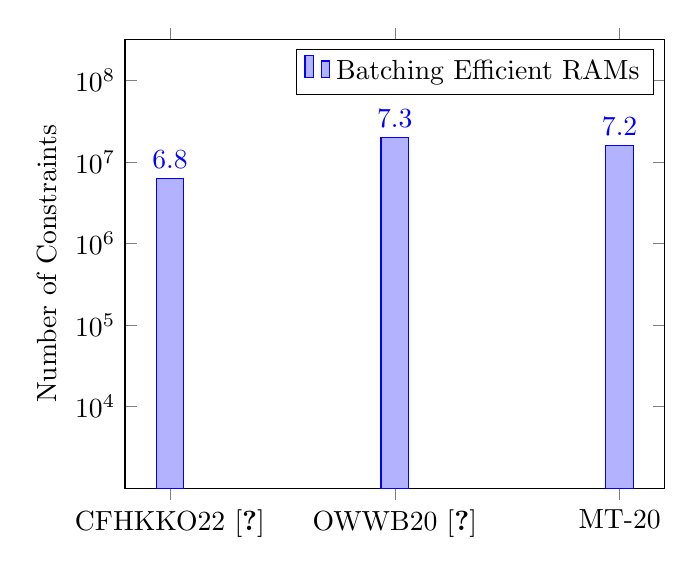
\begin{tikzpicture}
	        \begin{axis}[
	        ybar,
	        ylabel={Number of Constraints},
	        ymin = 3,
	        ymax = 8.5,
	        ytick = {4, 5, 6, 7, 8},
	        xlabel={},
	        xtick=data,
	        symbolic x coords= {A, B, C},
	        xticklabels = {CFHKKO22~\cite{CCS:CFHKKO22}, OWWB20~\cite{USENIX:OWWB20}, MT-20},
	        yticklabels = {$10^4$, $10^5$, $10^6$, $10^7$, $10^8$},
	        xlabel near ticks,
	        ylabel near ticks,
	        nodes near coords,
	        nodes near coords align={vertical},
	        ]
	        \addplot coordinates {(A,6.8) (B,7.3) (C,7.2)};
	        \legend{Batching Efficient RAMs}
	        \end{axis}
   	 \end{tikzpicture}
    \caption{Comparison of R1CS constraints incurred by existing approaches for batching efficient
    RAMs. MT20 refers to Merkle-tree with depth 20, instantiated using Poseidon hash.}
    \label{fig:batch-ram-constraints}
    \vspace*{-5mm}
\end{figure}

\begin{figure}[t!]
    \centering
	    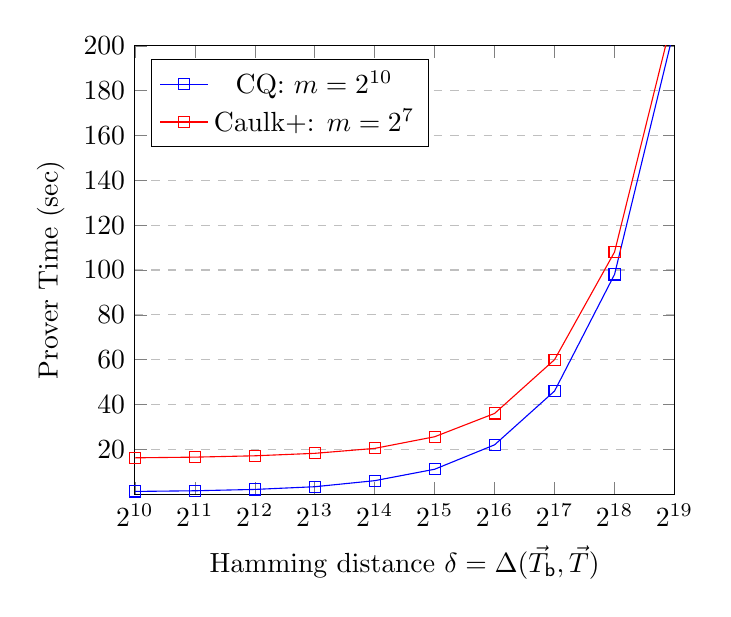
\begin{tikzpicture}
	        \begin{axis}[
	        xmin=0,
	        xmax=9,
	        ymin=0,
	        ymax=200,
	%		xlabel style={text width=0.5cm}, 
			xlabel= {Hamming distance $\delta = \Delta(\vecTbase,\vecT)$},
	        ylabel={Prover Time (sec)},
	        xtick={0, 1, 2, 3, 4, 5, 6, 7, 8, 9},
	        ytick={20, 40, 60, 80, 100, 120, 140, 160, 180, 200},
	        xticklabels={$2^{10}$, $2^{11}$, $2^{12}$, $2^{13}$, $2^{14}$, $2^{15}$, $2^{16}$, $2^{17}$, $2^{18}$, $2^{19}$},
	        yticklabels={20, 40, 60, 80, 100, 120, 140, 160, 180, 200},
	        legend pos=north west,
	        ymajorgrids=true,
	        grid style=dashed,
	        xlabel near ticks,
	        ylabel near ticks
	        ]
	        \addlegendimage{color=blue, mark=square}
	        \addlegendentry{CQ: $m=2^{10}$}
	        \addlegendimage{color=red, mark=square}
	        \addlegendentry{Caulk+: $m=2^{7}$}
	        \addplot[
	            color=blue,
	            mark=square,
	        ]
	        coordinates {
	            (0,1.2)(1,1.5)(2,2.1)(3,3.3)(4,6.0)(5,11.1)(6,22.0)(7,46)(8,98)(9,208)
	        };
	
	        \addplot[
	            color=red,
	            mark=square,
	        ]
	        coordinates {
	            (0,16.2)(1,16.5)(2,17.1)(3,18.2)(4,20.4)(5,25.6)(6,36)(7,60)(8,108)(9,216)
	        };
	        \end{axis}
	    \end{tikzpicture}
    \caption{Online proving time of updates on table $\vecT$ given the pre-processing parameters for table $\vecTbase$, plotted against the Hamming distance $\delta$ between $\vecTbase$ and $\vecT$. Here $m$ denotes the batch size of updates, while the RAM size is $N=2^{20}$. The blue plot corresponds to our scheme instantiated with CQ as the sub-vector argument (in a black-box manner). The red plot corresponds to the non-black-box adaptation of Caulk+ described in Appendix~\ref{app:committed-index-lookup}.}
    \label{fig:batch-ram-proving-time}
    \vspace*{-3mm}
\end{figure}

In this section we present a concrete evaluation of our batching efficient RAM and compare it to the
prior works on batching efficient RAM~\cite{USENIX:OWWB20,CCS:CFHKKO22}.
We also separately benchmark the effectiveness of our approach of computing encoded quotients presented
in Section~\ref{sec:update-protocol} over the na\"{i}ve approach.
 %on the experimental evaluation of our batching-efficient RAM.
%In addition, we also report on the overhead (as a function of changes since last parameter computation)
%incurred by our updatable lookup arguments over the vanilla lookup arguments with read-only table. We
%benchmark this overhead over vanilla implementations of Caulk+~\cite{EPRINT:PosKat22} and
%CQ~\cite{EPRINT:EagFioGab22}, both of which we also implement (as their non zero-knowledge variants)
%for our evaluation.
Our implementation is built on top of existing implementation~\cite{caulk-implementation}
of lookup argument Caulk~\cite{CCS:ZBKMNS22}. We make our implementation available at
\url{https://github.com/nitsatiisc/caulk/tree/updateable-ram}. 
%for anonymous submission. 
%We later plan to
%make the implementation available as open-source project.

\paragraph{\bf Experimental Test-bed.} All the benchmarks were run single-threaded on a commodity configuration featuring a
$2.1GHz$ Intel-I5 processor, $16$ GB memory running Ubuntu Linux 22.04. The implementation was compiled using {\tt --release}
flag in Rust. Our protocol was instantiated for BLS12-381 curve, using the scheme CQ~\cite{EPRINT:EagFioGab22}
as the underlying sub-vector argument.

\paragraph{\bf Online Proof Generation.} In Figure~\ref{fig:batch-ram-proving-time}, we benchmark the time
to prove a batch of $m=2^{10}$ updates on a table of size $N=2^{20}$. Here, the values on the $x$-axis denote
the hamming distance between the table on which the updates are being proved and the table whose pre-processed
parameters are used for the proof generation. Naturally, we expect the proving time to increase as the table
becomes more distant from the one used to generate pre-processed parameters. Our proof generation time stays
under a minute till the two table differ in almost $2\times 10^5$ positions. In conjunction with offline
pre-processing time from table~\ref{tbl:offline-proving-time}, the graph in Figure~\ref{fig:batch-ram-proving-time}
determines how the offline parameter generation should be scheduled to achieve optimal performance on average.

\paragraph{\bf Offline Pre-Processing.} In Table~\ref{tbl:offline-proving-time} we provide the time to compute
table-specific parameters as a function of table size. This is the most computationally intensive step in our
scheme involving FFTs over group polynomials as the main bottle-neck. We believe offline pre-processing can be
made an order of magnitude more efficient by leveraging parallel implementation for the FFTs.

\begin{table}[htbp]
	\centering
    \begin{tabular}{|l|c|c|c|c|c|c|}
        \hline
        \cellcolor{lightgray} Table-Size ($N$) & $2^{10}$ & $2^{12}$ & $2^{14}$ & $2^{16}$ & $2^{18}$ & $2^{20}$ \\ \hline
        \cellcolor{lightgray} Time (s) & $7$ & $29$ & $135$ & $620$ & $2766$ & $12000$ \\ \hline
    \end{tabular}
    \caption{Pre-processing time for tables of different sizes.}
    \label{tbl:offline-proving-time}
%    \vspace*{-5mm}
\end{table}


\noindent{\bf Proof Size and Verification Costs.} Our proof sizes and verification costs are independent of the
size of the table and the number of updates in a batch. For the instantiation of our scheme with BLS12-381 curve,
we incur a proof size of $4.4KB$ while the verification takes around $15ms$.

\paragraph{\bf Fast Update Benchmarks.} We also benchmark the efficiency of the algorithm to compute
 scalar coefficients in Lemma~\ref{lem:sum-computation}, required to assemble the encoded quotients from pre-computed quotients.
This algorithm is implemented and tested in the {\tt fastupdate} module of the referenced repository.
In Table~\ref{tbl:sum-computation-compare}, we compare it against the naive computation of the quotients.
In the table, we vary the sizes of set $I$ in Lemma~\ref{lem:sum-computation} in the set $\{2^i:7\leq i\leq 10\}$
and set $K=2^7|I|$. %i.e, we compare the two methods to sustain $\approx 100$ online proofs.
We clearly see $5\times-20\times$ advantage over the naive computation.

\paragraph{\bf Continuity.} To maintain {\em continuity} of the system~(this is particularly important for applications such as rollups), we must carefully
align the online prover performance curve with the cost of offline computation.  As an example, suppose $\vec{T}_0$
is the initial pre-processed table at time $t=0$. We generate proofs using pre-computed parameters for $\vec{T}_0$
till the time $t=t_1$, when the table state $\vec{T}_1$ is at hamming distance $2^{17}$ from $\vec{T}_0$. At this point,
from Figure~\ref{fig:batch-ram-proving-time}, online proof generation takes around $40s$ for batch of $1000$ updates.
At $t=t_1$, we also start an offline parameter computation for the table $\vec{T}_1$, while continuing to generate
online proofs using parameters for $\vec{T}_0$. We can generate the next $2^7$ batches of updates at an average of
approximately $12000/128\approx 94s$ each, thus finishing with a table state $\vec{T}_2$ at hamming distance at most
$2^{18}$ from $\vec{T}_0$ at $t_2=t_1+12000$. At this point, we should have the pre-computed parameters for $\vec{T}_1$,
which is at update distance of $2^{17}$ from $\vec{T}_2$, and thus online proof generation can switch to parameters
for the table $\vec{T}_1$. This alignment gives us a proving time of $94s$ per batch of $1000$, while ensuring system
is live at all times. Clearly, a faster offline pre-computation using parallel implementation would allow us to stay
at the cheaper end of online proving performance.


\begin{table}[htbp]
    \centering
    \begin{tabularx}{0.45\textwidth}{@{}XXXX@{}}
        \toprule
        $|I|$ & $|K|$ & Lemma~\ref{lem:sum-computation} & Naive \\ \midrule
        $2^7$ & $2^{14}$ & 3.3s  & 12s \\
        $2^8$ & $2^{15}$ & 7.7s  & 48s \\
        $2^9$ & $2^{16}$ & 16.8s & 198s \\
        $2^{10}$ & $2^{17}$ & 39.2s & 839s \\
        \bottomrule
    \end{tabularx}
    \caption{Comparison of Lemma~\ref{lem:sum-computation} and naive computation for calculating
    scalar coefficients for encoded quotients.}
    \label{tbl:sum-computation-compare}
    \vspace*{-5mm}
\end{table}

\noindent{\bf Comparison with Prior Works}. The proof generation in the prior batching efficient RAM constructions
using RSA accumulators~\cite{USENIX:OWWB20,CCS:CFHKKO22} involves two key steps (i) generation of a SNARK
proof showing knowledge of witness for a relation modeled as arithmetic circuit/R1CS and (ii) computing the witness
for the proof generation. A platform agnostic metric to express the cost of the first step is the number of R1CS
constraints needed to encode the relation, which is also the metric used in~\cite{CCS:CFHKKO22} for comparison.
Using the R1CS constraints reported in~\cite{USENIX:OWWB20,CCS:CFHKKO22} (see Figure~\ref{fig:batch-ram-constraints}),
we benchmark single-threaded proof generation
using the \textsf{Groth16} protocol (used in prior works) for R1CS of equivalent size on our test-bed. We use publicly
available benchmarking suite in~\cite{ark-groth-16} for \textsf{Groth16} benchmarks. Since the
the prior works only report performance of parallel implementation of the second step which is common to both (with
degree of parallelism not explicitly mentioned), we will use the reported parallel performance to estimate the
overall proving time with this caveat. 

Even without the benefit of parallelization, our average proof generation
time of $\approx 90s$ for batch size of $2^{10}$ and RAM size of $2^{20}$ is $3-5\times$ faster than the prior works
for the same setting. The proof sizes and verification complexity are constant for prior work and our work.
Concrete proof sizes are smaller in~\cite{USENIX:OWWB20,CCS:CFHKKO22} owing to their usage of \textsf{Groth16}
proving backend, while our verification times are competitive with~\cite{USENIX:OWWB20} and substantially
less than~\cite{CCS:CFHKKO22}. One way to reduce proof size in our scheme would be to use a SNARK to prove
memory-checking on smaller sub-RAMs, instead of explicit polynomial protocol that we employ for the same. For
completeness, we also include the batching efficient RAM using Merkle tree (with Poseidon hash) in the performance
comparison in Table~\ref{tbl:performance-comparison} which was considered in prior works. Note that the Merkle
 tree-based approach is faster than that of~\cite{USENIX:OWWB20} for batch size of $2^{10}$ (the break-even
 point reported to be batch size of $\approx 1200$).

\begin{table}[htbp]
    \centering
    \begin{tabularx}{0.8\textwidth}{@{}XXXX@{}}
        \toprule
        Scheme & $\prover$ (s) & $\verifier$ (ms) & $|\pi|$ (KB) \\ \midrule
        MT20 & $450$ & $7$  & $0.26$ \\
        OWWB20~\cite{USENIX:OWWB20} & $550+43$ & $7$  & $0.26$ \\
        CFHKKO22~\cite{CCS:CFHKKO22} & $226+43$ & $120$ & $1.3$ \\
        Our Work & $94$ & $15$ & $4.4$ \\
        \bottomrule
    \end{tabularx}
    \caption{Comparing performance of our batching-efficient RAM with prior works. $\prover$
    denotes proof generation time, $\verifier$ denotes verification time while $|\pi|$ denotes
    argument size. We mention proof generation time as $a+b$ for~\cite{USENIX:OWWB20,CCS:CFHKKO22}
    where $a$ denote proving time of \textsf{Groth16} and $b$ denotes witness generation time. The latter
    is reported in respective works for a parallel implementation.}
    \label{tbl:performance-comparison}
    \vspace*{-5mm}
\end{table}


%Generating table specific parameters for table of size $1$ million takes around $12,000$
%seconds for CQ based instantiation.

%We first provide overall running time of batching-efficient RAM primitive instantiated with Caulk+
%and CQ lookup arguments. The degradation in running time is plotted as function of accumulated updates
%since the last computation of full table-specific parameters in Figure~\ref{fig:batch-ram-proving-time}.
%We choose batch size of $m=128$ for Caulk+ based instantiation (to avoid prohibitive performance),
%while we consider $m=1024$ for CQ based instantiation. Our overhead remains barely noticable against
%the quadratic costs incurred by Caulk+ base protocol till about $2^{15}$ accumulated changes, equivalent of
%$128$ lookups of size $512$. While the performance overhead compared to base CQ protocol is much more apparent,
%overall we continue to achieve online proof generation time of under a minute all the way upto
%$\approx 2\times 10^5$ accumulated changes, equivalent of roughly $200$ batch updates (assuming the worst-case
%scenario). In real application scenarios, we can expect better degradation curve, as its unlikely that updates
%to the table occur uniformly across all positions.

%In Figure~\ref{fig:batch-ram-constraints}, we compare the
%R1CS constraints incurred by existing approaches to batching friendly RAMs/accumulators. For our work, we assume
%that the memory checking on the RAM instance of size $m$ is implemented as an arithmetic circuit using a Bene's
%routing network~\cite{benes}, though we also provide a purely polynomial protocol for the same in Section~\ref{sec:poly-proto-ram-app}.
%Our construction is relatively ``circuit-free'' and relies on the efficiency of lookup arguments coupled with
%our novel modifications to make them update resilient.






\bibliographystyle{plain}
\bibliography{cryptobib/abbrev3,cryptobib/crypto,main}

\appendix
\appendix

\section{Argument for RAM From Polynomial Protocols}\label{sec:poly-proto-ram-app}
In this section, we give a self-contained argument of knowledge for membership in the language
$\LRAM{I}{m}{m}$ introduced in Section \ref{sec:model-for-ram}. We first consider the polynomial encoding
of different RAM artefacts.
\subsection{Polynomial Encoding}\label{subsec:poly-encoding}
%The aim of this section is to encode artefacts such as RAM state, operations and transcripts as polynomials, and
%translate checking memory consistency (equivalently, checking membership in $\LRAM{I}{n}{m}$) to checking polynomial identities
%over the encoded polynomials. For
%simplicity and its usefulness later, we consider the case $m=n$, and accordingly check the membership in the language $\LRAM{I}{m}{m}$.
Let $k=3m$ and let $\omega$ be a primitive $k^{th}$ root of unity in $\F$.
Let $\nu=\omega^3$, and thus $\nu$ is a primitive $m^{th}$ root of unity in $\F$ (We assume, these roots exist in $\F$).
We recall $\setV$ as the subgroup consisting of $m^{th}$ roots of unity with associated Lagrange basis polynomials
$\{\tau_i(X)\}_{i\in [m]}$, while we additionally introduce the set $\setH$ of $k^{th}$ roots of unity with
$\{\lambda_i(X)\}_{i\in [k]}$ as the associated Lagrange polynomials.
\begin{gather}\label{eq:interpolation-sets}
\setH = \{\omega,\ldots,\omega^k\},\quad \setV = \{\nu,\ldots,\nu^m\}
\end{gather}
As before, we define the encoding of vectors in $\vec{f}\in \F^k$ as $\enc{f}{\setH}=\sum_{i\in [k]}f_i\lambda_i(X)$.
%Let $\{\lambda_i(X)\}_{i=1}^k$ be lagrange basis polynomials
%for the set $\setH$ and $\{\tau_i(X)\}_{i=1}^m$ be the lagrange polynomials for the set $\setV$ satisfying
%$\lambda_i(\omega^j)=\delta_{ij}$ for $i,j\in [k]$ and $\tau_i(\nu^j)=\delta_{ij}$ for $i,j\in [m]$.
%We use $\setH$ to encode a vector $\vec{f}=(f_1,\ldots,f_k)$ of size $k$ as the polynomial $f(X)\in \F_{<k}[X]$ such that $f(\omega^i)=f_i$ for $i\in [k]$.
%Similarly, we use $\setV$ to encode a vector
%$\vec{g}=(g_1,\ldots,g_m)$ of size $m$ as the polynomial $g(X)\in F_{<m}[X]$ such that $g(\nu^i)=g_i$ for $i\in [m]$. We use
%the notation $\enc{f}{\setH}$ and $\enc{g}{\setV}$ to denote polynomial encodings of vectors $\vec{f}\in \F^k$ and $\vec{g}\in \F^m$
%respectively.
%In the other direction, for a polynomial $f(X)\in \F[X]$,
%we use $\vec{f}_{|_\setH}$ and $\vec{f}_{|_\setV}$ to denote the vectors $(f(\omega^1),\ldots,f(\omega^k))$ and $(f(\nu^1),\ldots,f(\nu^m))$ respectively.
%The encoding of vectors as polynomials can be succinctly described using lagrange basis polynomials.
%Then we have $\enc{f}{\setH}=\sum_{i=1}^k f_i\lambda_i(X)$ and $\enc{g}{\setV}=\sum_{i=1}^m g_i\tau_i(X)$.
We canonically extend the encoding of vectors to encode RAM, operations and transcripts by encoding their component vectors.
Thus, for a RAM $T=(\vec{a},\vec{v})\in \RAM{I}{m}$, we define its encoding
$\wt{T}=(a(X),v(X))$ where $a(X),v(X)\in \F_{<m}[X]$ encode vectors $\vec{a}, \vec{v}$ respectively.
Given an operation sequence
$\vec{o}=(o_1,\ldots,o_m)$ with $o_i=(\bar{\op}_i,\bar{a}_i,\bar{v}_i)$ we encode $\vec{o}$ as
$\wt{O}$ $=$ $(\bar{\op}(X)$ ,$\bar{a}(X)$ ,$\bar{v}(X))$
where $\bar{\op}(X)$ encodes the
vector $\vec{\op}=(\bar{\op}_1,\ldots,\bar{\op}_m)$, $\bar{a}(X)$ encodes the vector $(\bar{a}_1,\ldots,\bar{a}_m)$ and
$\bar{v}(X)$encodes the vector $(\bar{v}_1,\ldots,\bar{v}_m)$.
Finally, a transcript $\tr=(\vec{t},\vec{\op},\vec{A},\vec{V})$ for tuples $(T,\vec{o},T')$ where $T,T'$ are RAMs of size $m$,
and $\vec{o}$ is an operation sequence of size $m$ is encoded as $\wt{\tr}$ $=$ $(t(X)$, $\op(X)$, $A(X)$, $V(X))$
where the polynomials $t(X),\op(X),V(X)$ and $A(X)$ encode the respective vectors in $\F^k$ (See Section \ref{sec:model-for-ram}).

\subsection{Relations over Polynomial Encodings}\label{subsec:encoded-relations}
In this section, we describe polynomial checks for two important relations we need in subsequent sections, viz,
(i) checking concatenation of vectors and (ii) checking monotonicity and load-store consistency of a transcript.
The lemma below specifies the polynomial identities for verifying
that vector $\vec{v}\in \F^k$ is concatenation of vectors $\vec{a},\vec{b},\vec{c}$ in $\F^m$.

\begin{lemma}\label{lem:vec-concatenation}
Let $\vec{a},\vec{b},\vec{c}\in \F^m$  and $v\in \F^k$ be vectors encoded by polynomials
$a(X),b(X),c(X)$ and $v(X)$ respectively. Then,
\begin{align}
    a(X^3) - v(X)  &= 0  \quad \text{ mod $Z(X)$ } \tag{A1}\label{eq:A1}\\
    b(X^3) - v(\omega^m X)  &= 0   \quad \text{ mod $Z(X)$ } \tag{A2}\label{eq:A2}\\
    c(X^3) - v(\omega^{2m} X) &= 0 \quad \text{ mod $Z(X)$ } \tag{A3}\label{eq:A3}
\end{align}
for $Z(X)=\prod_{i=1}^m (X-\omega^i)$ if and only if $\vec{v}=\vec{a}||\vec{b}||\vec{c}$.
\end{lemma}
\begin{proof}
    Assume that the polynomial identities hold. Substituting $X=\omega^i$ for $i\in [m]$ in above equations implies
    for $i\in [m]$: $a_i=v_i$ (Eq \eqref{eq:A1}), $b_i=v_{m+i}$ (Eq \eqref{eq:A2}) and $c_i=v_{2m+i}$ (Eq \eqref{eq:A3}),
    which together imply $\vec{v}=\vec{a}||\vec{b}||\vec{c}$. Converse follows by observing that $\vec{v}=\vec{a}||\vec{b}||\vec{c}$
    implies that $v(X) = a(X^3)$, $v(\omega^m X)=b(X^3)$ and $v(\omega^{2m} X)=c(X^3)$ holds for all $X=\omega^i, i\in [m]$.
    Thus, the equalities hold modulo the polynomial $Z(X)$ as defined above.
\end{proof}

Next, we specify polynomial checks on the encoding of a transcript to ensure it satisfies address-ordering and load-store consistency.
Let $N$ be an upper bound on the values of $\vec{A}$, i.e, the index set $\setind\subseteq [N]$.
Let $\tr=(\vec{t},\vec{\op},\vec{A},\vec{V})$ be a transcript encoded as
$\wt{\tr}=(t(X),\op(X),A(X),V(X))$. Recall that we need to check two conditions on $\tr$, viz, (i) {\em monotonicty}:
the transcript is sorted by address and timestamp respectively, i.e, $A_i\leq A_{i+1}$ for all $i < k$ and
$t_i < t_{i+1}$ whenever $A_i=A_{i+1}$, (ii) {\em load-store consistency}: whenever $\op_{i+1}=0$ and $A_i=A_{i+1}$,
we have $V_i=V_{i+1}$.
To do so, we exhibit disjoint sets $I_1,I_2$ with $I_1\uplus I_2=[k]$ such that: (i) for all
$i\in I_1$, $A_i < A_{i+1}$, (ii) for all $i\in I_2$, $(A_i = A_{i+1})\wedge (t_i < t_{i+1})$ and (iii) for all $i\in I_2$,
$(\op_i=1)\vee (V_i = V_{i+1})$. We vacuously allow $k$ to be part of either of the sets.
Note that the conditions on the sets $I_1$ and $I_2$ ensures monotonicity.
Moreover, it can be seen that load-store consistency requirements are satisfied for all $i\in I_1$ (as $A_i\neq A_{i+1}$).
Similarly,load-store consistency also holds for all $i\in I_2$.
It remains to exhibit the sets and show that they satisfy the above invariants using polynomials, as in the following
lemma:
\begin{lemma}\label{lem:addr-ordered-transcript}
Let $\wt{\tr}$ be a polynomial encoding of transcript $\tr$ of size $k$, given by polynomials $t(X),\op(X),A(X)$ and $V(X)$,
with index set $[N]$. Then assuming $kN<|\F|$, $\tr$ is address ordered and satisfies load-store consistency if and only if there exist polynomials
$Z_1,Z_2,\delta_T,\delta_A$
such that the following hold:
\begin{align}%\label{eq:loadstore-consitency-constraints}
    & Z_2(X)(A(\omega X) - A(X) - \delta_A(X)) = 0 \text{ mod } \mathbb{Z}_\setH(X) \tag{C1} \label{eq:C1} \\
    & A(\omega X) - A(X) = 0  \text{ mod } Z_2(X) \tag{C2} \label{eq:C2} \\
    & t(\omega X) - t(X) - \delta_T(X) = 0  \text{ mod } Z_2(X) \tag{C3} \label{eq:C3} \\
    & (\op(X) - 1)(V(\omega X) - V(X)) = 0  \text{ mod } Z_2(X) \tag{C4} \label{eq:C4} \\
    & Z_1(X)\cdot Z_2(X) = \mathbb{Z}_\setH(X) \quad  \tag{C5} \label{eq:C5} \\
    & 1\leq A(\omega^i) \leq N  \quad \tag{C6} \label{eq:C6} \\
    & 1\leq t(\omega^i) \leq N, 1\leq \delta_A(\omega^i)\leq N,\ 1\leq \delta_T(\omega^i)\leq N \text{ for } i\in [k] \tag{C7} \label{eq:C7}
\end{align}
\end{lemma}
\begin{proof}
Suppose there exist polynomials $Z_1(X),Z_2(X),\delta_T(X)$ and $\delta_A(X)$ satisfying above identities. From Equation
~\eqref{eq:C5}, we conclude that their exist sets $I_1,I_2$ with $I_1\uplus I_2=[k]$ such that $Z_b(X)$, $b\in \{0,1\}$ is the
    vanishing polynomial of the set $\{\omega^i: i\in I_b\}$. We now note that the following are true for $i\in I_1$:
    \begin{itemize}[leftmargin=1em]
        \item $A(\omega^{i+1})-A(\omega^i)=\delta_A(\omega^i)$. Since $1\leq \delta_A(\omega^i)\leq N$, this ensures $A_i < A_{i+1}$ for the vector $\vec{A}$ encoded
        by $A(X)$. We note that $kN < |\F|$ implies there is no overflow modulo the field characteristic.
    \end{itemize}
    Similarly, it can be seen that for $i\in I_2$, we must have (i) $A_i=A_{i+1}\wedge t_i < t_{i+1}$
    and (ii) $\op_i=1\,\vee\,V_i=V_{i+1}$. Together these imply that the encoded transcript is address-ordered.
\end{proof}

\begin{figure}[htbp]
	\centering
	\begin{mdframed}
		{\small
			\noindent{\bf Common Input}: Commitments $c_t$, $c_{op}$, $c_A$ and $c_V$ to $t,op,A$ and $V$ respectively. 
			\begin{enumerate}[leftmargin=2em]
				\item $\prover\rightarrow\verifier$: $\prover$ sends $\gone{\Z_\setH}$, $\gone{Z_2}$, $\gone{\delta_T}$, $\gone{\delta_A}$
				\item $\verifier\rightarrow\prover$: Verifier sends $\gamma\gets \F$.
				\item $\prover$ computes:
				\begin{align}
					& Q_1(X) =  Z_2(X) (A(\omega X) - A(X) - \delta_A(X)) / \Z_\setH(X)\\
					& Q_2(X) =  (A(\omega X) - A(X)) / Z_2(X) \\
					& Q_3(X) = (t(\omega X) - t(X) - \delta_T(X)) / Z_2(X) \\
					& Q_4(X) = (\op(X) - 1)(V(\omega X) - V(X)) / Z_2(X)
				\end{align}
				\item $\prover\rightarrow\verifier$: Sends commitment $\gone{Q_1}$, $\gone{Q_2}$, $\gone{Q_3}$ and $\gone{Q_4}$ to $Q_1(X)$, $Q_2(X)$, $Q_3(X)$ and $Q_4(X)$.
				\item $\verifier\rightarrow\prover$: Sends $s\gets\F$.
				\item $\prover\rightarrow\verifier$: Sends evaluations $\val{s}{A}=A(s)$, $\val{\omega s}{A}=A(\omega s)$, $\val{s}{\delta_A} = \delta_A(s)$, $\val{s}{t}=t(s)$, $\val{\omega s}{t}=t(\omega s)$, $\val{s}{\delta_T} = \delta_T(s)$, $\val{s}{\op}=\op(s)$, $\val{s}{V}=V(s)$, $\val{\omega s}{V}=V(\omega s)$, $\val{s}{Q_1}=Q_1(s)$, $\val{s}{Q_2}=Q_2(s)$, $\val{s}{Q_3}=Q_3(s)$, $\val{s}{Q_4}=Q_4(s)$, $\val{s}{Z_2}=Z_2(s)$, $\val{s}{\Z_\setH}=\Z_\setH(s)$.
%				\item $\prover\rightarrow\verifier$: Sends evaluations $\val{\omega^i}{A} = A(\omega^i)$, $\val{\omega^i}{t} = t(\omega^i)$, $\val{\omega^i}{\delta_A} = \delta_A(\omega^i)$ and $\val{\omega^i}{\delta_T} = \delta_T(\omega^i)$ for all $i\in [N]$
				\item $\verifier\rightarrow\prover$: Sends $r\gets\F$.
				\item $\prover\rightarrow\verifier$: Sends $\kzg$ proofs:
								\begin{itemize}[leftmargin=2em]
										\item $\Pi_{F_1}=\kzgprove(\srs,F_1,\omega s)$, where $F_1(X) = A(X) + r t(X) + r^2 V(X)$
										\item $\Pi_{F_2}=\kzgprove(\srs,F_2,s)$ where $F_2(X) = A(X) + r t(X) + r^2 \op(X) + r^4 V(X) + r^5 \delta_A + r^6 \delta_T(X) + r^7 Z_2(X) + r^8 \Z_\setH(X) + r^{9} Q_1(X) + r^{10} Q_2(X) + r^{11} Q_3(X) + r^{12} Q_4(X)$
%										\item $\Pi_{F_3}=\kzgprove(\srs,F_3,(\omega^i)_{i\in [N]})$, where $F_3(X)=A(X) + r t(X) + r^2 \delta_A(X) + r^3 \delta_T(X)$
									\end{itemize}
%				\item $\prover\rightarrow\verifier$: Sends $\rangeproof$ proofs:
%				\begin{itemize}[leftmargin=2em]
%					\item $\Pi_{F_1}=\rangeproof(\srs,[N],\val{\omega}{A})$
%				\end{itemize}
				\item $\verifier$ computes: Compute commitments $\gone{F_1}$ and $\gone{F_2}$ using homomorphism. It then checks:
								\begin{itemize}[leftmargin=2em]
									\item $\kzgverify(\srs,\gone{F_1},\omega s, \val{\omega s}{A}+r \val{\omega s}{t} + r^2 \val{\omega s}{V},\Pi_{F_1})$
									\item $\kzgverify(\srs,\gone{F_2}, s, \val{s}{A}=A(s) + r \val{s}{t}=t(s) + r^2 \val{s}{\op}=\op(s) + r^4 \val{s}{V}=V(s) + r^5 \val{s}{\delta_A}=\delta_A(s) + r^6 \val{s}{\delta_T}=\delta_T(s) + r^7 \val{s}{Z_2}=Z_2(s) + r^8 \val{s}{\Z_\setH}=\Z_\setH(s) + r^{9} \val{s}{Q_1}=Q_1(s) + r^{10} \val{s}{Q_2}=Q_2(s) + r^{11} \val{s}{Q_3}=Q_3(s) + r^{12} \val{s}{Q_4}=Q_4(s), \Pi_{F_2})$
%									\item $\kzgverify(\srs,\gone{F_3},(\omega^i)_{i\in [N]}, \big( \val{\omega^i}{A} + r \val{\omega^i}{t} + r^2 \val{\omega^i}{\delta_A} + r^3 \val{\omega^i}{\delta_T} \big)_{i\in [N]} ,\Pi_{F_3})$
									\item $\val{s}{Q_1}\cdot \val{s}{\Z_\setH} =? \val{s}{Z_2} (\val{\omega s}{A} - \val{s}{A} - \val{s}{\delta_A})$
									\item  $\val{s}{Q_2}\cdot \val{s}{Z_2} =? (\val{\omega s}{A} - \val{s}{A})$
									\item $\val{s}{Q_3}\cdot \val{s}{Z_2} =? (\val{\omega s}{t} - \val{s}{t} - \val{s}{\delta_A})$
									\item $\val{s}{Q_4}\cdot \val{s}{Z_2} =? (\val{s}{\op}-1)(\val{\omega s}{V} - \val{s}{V})$
								\end{itemize}
%				\item $\prover$ and $\verifier$ invokes 
				\item $\verifier$ outputs: Accept if all the above checks succeeds, otherwise it rejects.
			\end{enumerate}
		}
	\end{mdframed}
	%\vspace*{-5mm}
	\caption{Protocol: Check relations over polynomial encodings}
	\label{fig:encoded-relations}
\end{figure}

\begin{figure}[htbp]
	\begin{mdframed}
    {
			\noindent{\bf Common Input}: Commitments $c_a$, $c_b$, $c_c$, $c_v$, and $\gone{Z}$ (to the polynomial
			$Z(X)=\prod_{i=1}^m (X-\omega^i)$). \\
            \noindent{\bf Prover's Input}: Vectors $\vec{a},\vec{b},\vec{c}\in\F^m$ and $\vec{v}\in \F^k$.
			\begin{enumerate}[leftmargin=1em, label=\arabic*.]
				\item $\verifier$ sends $\gamma\gets \F$.
				\item $\prover$ computes:
				\begin{align}
					& h(X) = a(X) + \gamma b(X) + \gamma^2 c(X),\\
					& Q(X) = (h(X^3) - v(X) - \gamma v(\omega^m X) - \gamma^2 v(\omega^{2m} X))/Z(X)
				\end{align}
				\item $\prover$ sends commitment $\gone{Q}$ = $\gone{Q(X)}$.
				\item $\verifier$ sends $s\gets\F$.
				\item $\prover$ sends evaluations $\val{s}{v}=v(s)$, $\val{\omega^m s}{v}=v(\omega^m s)$,
				$\val{\omega^{2m}s}{v}=v(\omega^{2m} s)$, $\val{s^3}{h}=h(s^3)$, $\val{s}{Q}=Q(s)$ and $\val{s}{Z}=Z(s)$.
				\item $\verifier$ sends $r\gets\F$.
				\item $\prover$ computes $\kzg$ proofs:
				\begin{itemize}[leftmargin=1em]
					\item $\Pi_v=\kzgprove(\srs,v,(s,\omega^m s, \omega^{2m}s))$.
					\item $\Pi_h=\kzgprove(\srs,h,s^3)$.
					\item $\Pi_f=\kzgprove(\srs,f,s)$ where $f(X)=Z(X) + rQ(X)$.
				\end{itemize}
                \item $\prover$ sends $\Pi_v$, $\Pi_h$ and $\Pi_f$.
				\item $\verifier$ Computes commitments $\gone{h}$ and $\gone{f}$ using homomorphism.
                \item $\verifier$ checks:
				\begin{itemize}[leftmargin=1em]
					\item $\kzgverify(\srs,\gone{v},\vec{p}_v, \vec{e}_v, \Pi_v)$ where
                    $\vec{p}_v$ = $(s,\omega^m s, \omega^{2m}s)$ and $\vec{e}_v$ = $(\val{s}{v}, \val{\omega^m s}{v}, \val{\omega^{2m} s}{v})$.
					\item $\kzgverify(\srs,\gone{h}, s^3, \val{s^3}{h},\Pi_h)$.
					\item $\kzgverify(\srs,\gone{f}, s, \val{s}{Z} + r\val{s}{Q}, \Pi_f)$.
					\item $\val{s}{Q}\cdot \val{s}{Z} =? \val{s^3}{h}-\val{s}{v}-\gamma \val{\omega^m s}{v}-\gamma^2\val{\omega^{2m}s}{v}$.
				\end{itemize}
				\item $\verifier$ outputs accept if all the above checks succeed, else it rejects.
			\end{enumerate}
		}
	\end{mdframed}
	%\vspace*{-5mm}
	\caption{Protocol: Check concatenation via commitments}
	\label{fig:concatenation}
\end{figure}

\section{Succinct Argument for Verifiable RAM}\label{sec:poly-proto-ram}
The polynomial encodings in the previous section can be used to polynomial protocol for
checking the membership in the language $\LRAM{I}{m}{m}$ for $m\in \N$. The polynomial protocol can be subsequently
be compiled into a succinct argument using an extractable polynomial commitment scheme.
In this section, we use $\kzg$ polynomial commitment scheme to obtain a succinct argument for checking membership in $\LRAM{I}{m}{m}$
in the Algebraic Group Model (AGM).
At a high level, to prove $(\vec{T},\vec{o},\vec{T'})\in \LRAM{I}{m}{m}$, the prover
constructs time ordered transcript $\tr$ and then permutes it to obtain the address sorted transcript $\tr^\ast$.
It then sends the polynomial encodings of $\vec{T},\vec{o},\vec{T'},\tr$ and $\tr^\ast$ to the verifier, who verifies that:
\begin{enumerate}[leftmargin=1em]
    \item The time ordered transcript is correctly constructed, i.e, $\tr=\TOT(\vec{T},\vec{o},\vec{T'})$.
    \item The transcript $\tr^\ast$ is a permutation of the transcript $\tr$, i.e, $\tr^\ast=\sigma(\tr)$ for some permutation $\sigma$ of $[k]$.
    \item The transcript $\tr^\ast$ is address ordered and satisfies load-store consistency.
\end{enumerate}
In fact, we consider memebership in the above language under commitments. Let $\srs$ denote a $\kzg$ setup over a bilinear group, with
prime order groups $\Gone, \Gtwo$ and $\GT$. We canonically commit to RAM, operation sequences and transcripts by committing to their
polynomial encodings. Commitment of an encoding represented as tuple of polynomials is simply the tuple consisting of commitments of the component
polynomials. We now define
the relation $\CLRAM$ below, and present a succinct argument for the same.
\begin{definition}\label{defn:committed-vram}
Let $\CLRAM$ consist of tuples $((c_T, c_o, c_T'), (T, \vec{o},T'))$ where $c_T$ $=$ $\kzgcommit(\srs, \wt{T})$,
$c_T'$ $=$ $\kzgcommit(\srs, \wt{T'})$,
$c_o$ $=$ $\kzgcommit(\srs,\wt{O})$ commit to $T$, $T'$ and $\vec{o}$ with $(T,\vec{o},T')\in \LRAM{I}{m}{m}$.
\end{definition}
\noindent In the above definition we have $c_T=(c_a,c_v)$ where $c_a$ and $c_v$ are $\kzg$ commitments to polynomials $a(X)$ and $v(X)$ in
the encoding $\wt{T}=(a(X), v(X))$. Similarly we parse $c_T'=(c_a', c_v')$ and $c_o=(\bar{c}_\op, \bar{c}_a, \bar{c}_v)$ (see Section
\ref{subsec:poly-encoding} for polynomial encodings).
For proving relation \ref{defn:committed-vram}, prover's input consists of initial RAM state $T=(\vec{a},\vec{v})$,
final RAM state $T'=(\vec{a'},\vec{v'})$, operation sequence $\vec{o}=(o_1,\ldots,o_m)$ with $o_i=(\bar{\op}_i,\bar{a}_i,\bar{v}_i)$,
time-ordered transcript $\tr=(\vec{t},\vec{\op},\vec{A},\vec{V})$ and address-ordered transcript $\tr^\ast=(\vec{t^\ast},\vec{\op^\ast},
\vec{A^\ast},\vec{V^\ast})$ obtained from $\tr$ using a permutation $\sigma:[k]\rightarrow [k]$. Verifier's input consists of the
commitments $c_T, c_o$ and $c_T'$ as described above.

The prover starts the protocol by sending commitments $c_\tr$ and $c^\ast_\tr$ to the transcripts $\tr$ and $\tr^\ast$ respectively.
To show that $\tr$ is correctly formed, the prover needs to prove the concatenations:
(i) $\vec{\op}=0^m||(\bar{\op}_1,\ldots,\bar{\op}_m)||0^m$, (ii) $\vec{A}=\vec{a}||(\bar{a}_1,\ldots,\bar{a}_m)||\vec{a'}$
and (iii) $\vec{V}=\vec{v}||(\bar{v}_1,\ldots,\bar{v}_m)||\vec{v'}$. Note that the time-stamp column $\vec{t}$ is implicitly assumed
to be $(1,\ldots,k)$.
The verifier checks the concatenations using Lemma \ref{lem:vec-concatenation}.
It uses a random challenge $\beta$ to reduce the three concatenations to one concatenation, and uses another challenge $\gamma$
to reduce the three polynomial checks in Lemma \ref{lem:vec-concatenation} to a single check.
The complete polynomial protocol is detailed in Figure \ref{fig:time-ordered-transcript}.

%\begin{tcolorbox}
\begin{figure}[htbp]
    \centering
    \begin{mdframed}
    {\footnotesize
    \noindent{\bf Common Input}: Commitments $c_T=(c_a,c_v)$, $c_o=(\bar{c}_\op, \bar{c}_a, \bar{c}_v)$, $c_T'=(c_a', c_v')$
        and $c_\tr=(c_t, c_\op, c_A, c_V)$ to $T,o,T'$ and $\tr$ respectively. Commitment $\gone{Z}$ to the polynomial
        $Z(X)=\prod_{i=1}^m (X-\omega^i)$.
        \begin{enumerate}[leftmargin=2em]
            \item $\verifier\rightarrow\prover$: Verifier sends $\beta,\gamma\gets \F$.
            \item $\prover$ computes:
            \begin{align}\label{eq:poly-constraints}
            & G_1(X) = a(X) + \beta v(X),\, G_2(X) = \bar{a}(X) + \beta \bar{v}(X) + \beta^2 \bar{\op}(X) \tag{A1} \\
            & G_3(X) = a'(X) + \beta v'(X),\, G(X) = A(X) + \beta V(X) + \beta^2 \op(X) \tag{A2} \\
            & H(X) = G_1(X) + \gamma G_2(X) + \gamma^2 G_3(X), \tag{A3} \\
            & Q(X) = (H(X^3) - G(X) - \gamma G(\omega^m X) - \gamma^2 G(\omega^{2m} X))/Z(X) \tag{A4}
            \end{align}
            \item $\prover\rightarrow\verifier$: The prover sends commitment $\gone{Q}$ to $Q(X)$.
            \item $\verifier\rightarrow\prover$: Sends $s\gets\F$.
            \item $\prover\rightarrow\verifier$: Sends evaluations $\val{s}{G}=G(s)$, $\val{\omega^m s}{G}=G(\omega^m s)$,
            $\val{\omega^{2m}s}{G}=G(\omega^{2m} s)$, $\val{s^3}{H}=H(s^3)$, $\val{s}{Q}=Q(s)$ and $\val{s}{Z}=Z(s)$.
            \item $\verifier\rightarrow\prover$: Sends $r\gets\F$.
            \item $\prover\rightarrow\verifier$: Sends $\kzg$ proofs:
            \begin{itemize}[leftmargin=2em]
                \item $\Pi_G=\kzgprove(\srs,G,(s,\omega^m s, \omega^{2m}s))$.
                \item $\Pi_H=\kzgprove(\srs,H,s^3)$.
                \item $\Pi_F=\kzgprove(\srs,F,s)$ where $F(X)=Z(X) + rQ(X)$.
            \end{itemize}
            \item $\verifier$ computes: Compute commitments $\gone{G},\gone{H}$ and $\gone{F}$ using homomorphism. It then checks:
            \begin{itemize}[leftmargin=2em]
                \item $\kzgverify(\srs,\gone{G},(s,\omega^m s, \omega^{2m}s), (\val{s}{G}, \val{\omega^m s}{G}, \val{\omega^{2m} s}{G}),\Pi_G)$.
                \item $\kzgverify(\srs,\gone{H}, s^3, \val{s^3}{H},\Pi_H)$.
                \item $\kzgverify(\srs,\gone{F}, s, \val{s}{Z} + r\val{s}{Q}, \Pi_F)$.
                \item $\val{s}{Q}\cdot \val{s}{Z} =? \val{s^3}{H}-\val{s}{G}-\gamma \val{\omega^m s}{G}-\gamma^2\val{\omega^{2m}s}{G}$.
            \end{itemize}
            \item $\verifier$ outputs: Accept if all the above checks succeeds, otherwise it rejects.
        \end{enumerate}
    }
    \end{mdframed}
    \vspace*{-5mm}
    \caption{Protocol: Check correctness of time-ordered transcript}
    \label{fig:time-ordered-transcript}
\end{figure}
%\end{tcolorbox}

Next, we show a polynomial protocol for proving that the transcript $\tr^\ast$ is a permutation of the transcript $\tr$.
We first recall the permutation argument for vectors from ~\cite{EPRINT:GabWilCio19}.
\begin{lemma}[Permutation Check \cite{EPRINT:GabWilCio19}]\label{lem:perm-argument}
Let $f(X), g(X)$ be polynomials in $\F[\,X\,]$. Then, the vectors $\vec{f}, \vec{g}\in \F^k$ encoded by the polynomials
are permutations of each other if and only if with overwhelming probability over the choice of $\alpha\gets \F$,
there exists a polynomial $z(X)$ satisfying the polynomial constraints:
    {\small
\begin{align}
    \lambda_1(X)(z(X) -1) &= 0 \text{ mod } Z_\setH(X) \tag{B1} \label{eq:B1} \\
    (\alpha - g(X))z(\omega X) &= (\alpha - f(X))z(X) \text{ mod } Z_\setH(X) \tag{B2} \label{eq:B2}
\end{align}
}
\end{lemma}
The polynomial protocol in Figure \ref{fig:permutated-transcripts} essentially invokes the above argument on
the random linear combination of the columns of the respective transcripts.
%\begin{tcolorbox}
\begin{figure}[htbp]
    \centering
    \begin{mdframed}
    {\footnotesize
    \noindent{\bf Common Input}: Commitments $c_\tr=(c_t,c_\op,c_A, c_V)$ and $c_\tr^\ast=(c_t^\ast,c_\op^\ast, c_A^\ast, c_V^\ast)$
        of transcripts $\tr$ and $\tr^\ast$ respectively.
        \begin{enumerate}[leftmargin=2em]
            \item $\verifier\rightarrow\prover$: Sends $\alpha,\beta, \chi\gets \F$
            \item $\prover$ computes $f(X)=t(X) + \beta \op(X) + \beta^2 A(X) + \beta^3 V(X)$, $g(X) = t^\ast(X) + \beta \op^\ast(X)$
            $+ \beta^2 A^\ast(X) + \beta^3 V^\ast(X)$. It then computes polynomials $z(X),q(X)$ as:
            \begin{itemize}[leftmargin=1em]
                \item Interpolate polynomial $z(X)$ of degree $k-1$ such that $z(\omega)=1$ and
                $z(\omega^{i+1})=\prod_{j=1}^i (\alpha - f(\omega^j))/(\alpha - g(\omega^j))$ for $1\leq i\leq k$.
                \item Compute $q(X) = ((\alpha - g(X))z(\omega X) - (\alpha - f(X))z(X) + \chi\lambda_1(X)(z(X) - 1))/\mathbb{Z}_{\setH}(X)$.
            \end{itemize}
            \item $\prover\rightarrow\verifier$: Sends commitments $\gone{z}$ and $\gone{q}$ to polynomials $z(X)$ and $q(X)$ respectively.
            \item $\verifier$ computes: The verifier checks that $q(X)Z_\setH(X)$ = $(\alpha - g(X))z(\omega X)-(\alpha - f(X))z(X) + \chi\lambda_1(X)(z(X) - 1)$
            by requesting evaluations and $\kzg$ proofs of polynomials $f,g$ and $q$ at a random point. It accepts if the check succeeds.
        \end{enumerate}
    }
    \end{mdframed}
    \vspace*{-5mm}
    \caption{Protocol: Check permutation of transcripts}
    \label{fig:permutated-transcripts}
\end{figure}
%\end{tcolorbox}
Finally, we see that Lemma \ref{lem:addr-ordered-transcript} implies a polynomial protocol to check that the transcript
$\tr^\ast$ is address ordered and satisfies load-store consistency. We skip the formal protocol details, which
essentially involves the prover identifying sets
$I_1, I_2$ as described in Section \ref{subsec:encoded-relations} and sending auxiliary polynomials $Z_1(X),Z_2(X),\delta^\ast_A(X)$ and $\delta^\ast_T(X)$ to the verifier.
The verifier then checks the identities (C1)-(C6) in Lemma \ref{lem:addr-ordered-transcript}.
The range checks in (C7) can be checked using polynomial protocols in sub-vector lookup arguments such as Caulk+ ~\cite{EPRINT:PosKat22}, CQ
~\cite{EPRINT:EagFioGab22}. For completeness, we also include a protocol for enforcing range checks using committed index lookup
described in Section \ref{subsec:committed-index-lookup}.


\section{Proof of Lemma ~\ref{lem:sum-computation}}
%Recall the statement of lemma \ref{lem:sum computation}. We want to compute $e_i$ for all $i \in \setind$ and $b_j$ for all $j \in K$ in $O(|K|\log^2|K|)$ $\mathbb{F}$ operations.\\\\
Before starting the proof, we collect some preliminaries which will be useful in the proof.

\subsection{Computational Algebra Preliminaries}\label{subsec:comp-algebra-app}
Let $\F$ be a finite field of prime order $p$ and $\G$ be a cyclic additive group of order $p$ with generator $g$. For $s \in \F$, we use
the notation $\elt{s}$ to denote the group element $s\cdot g$. Assume that $\F$ contains $n^{th}$ root of unity $\xi$
satisfying $\xi^n=1$ for large $n$ (All polynomial degrees are assumed less than $n$).

\begin{fact}[\textsf{Fast Evaluation}]\label{fc:fft}
Let $f\in \F[X]$ be a polynomial of degree $<d$ and $(\xi_1,\ldots,\xi_r)\in \F^r$ be distinct points in $\F$.
Then the vector $(f(\xi_1),\ldots,f(\xi_r))$ can be computed in $O((d+r)\log (d+r))$ $\F$ operations if $\xi_1,\ldots,\xi_r$ form roots
of unity, and in $O((d+r)\log^2(d+r))$ $\F$ operations otherwise.
\end{fact}

\begin{fact}[\textsf{Fast Interpolation}]\label{fc:ifft}
Let $\xi_1,\ldots,\xi_d$ be distinct points in $\F$ and $(v_1,\ldots,v_d)\in \F^d$. Then $(f_0,\ldots,f_{d-1})\in \F^d$
can be computed in $O(d\log^2 d)$ operations in $\F$ such that $f(\xi_i)=v_i$ for all $i\in [d]$ where
$f(X)=\sum_{i=0}^{d-1}f_iX^i$.
\end{fact}

\begin{fact}[\textsf{Fast Multiplication}]\label{fc:mult}
Let $\xi_1,\ldots,\xi_r$ be distinct points in $\F$. Then coefficients of $f(X)=\prod_{i=1}^r (X-\xi_i)$
can be computed in $O(r\log^2 r)$ operations in $\F$.
\end{fact}

\begin{fact}[\textsf{Multi KZG proofs} ~\cite{EPRINT:FeiKho23}]\label{fc:multkzg}
Let $\{\elt{x^i}\}_{i=1}^d$ be given for some $x\in \F$. Then for set of $r$ distinct points $\xi_1,\ldots,\xi_r$,
and a polynomial $f(X)\in \F[X]$ of degree $<d$,the vector $(\elt{h_1(x)},\ldots,\elt{h_r(x)})$,
where $h_i(X) = (f(X) - f(\xi_i))/(X - \xi_i)$ can be computed in
$O((r+d)\log(r+d))$ group and field operations when $\xi_1,\ldots,\xi_r$ are roots of unity, and in
$O(rlog^2 r + d\log d)$ group and field operations otherwise.
\end{fact}

\begin{fact}[\textsf{Lagrange Polynomials}]\label{fc:lagrange}
Let $\mathbb{S}=\{\xi_1,\ldots,\xi_r\}$ be a set of $r$ distinct points and let $\tau_1(X),\ldots,\tau_r(X)$ be
the corresponding lagrange polynomials of degree $r-1$ each. Let $Z_{\mathbb{S}}(X)=\prod_{i=1}^r (X-\xi_r)$ denote the vanishing polynomial
for $\mathbb{S}$. Then we have:
\begin{gather*}
    \sum_{i=1}^r \tau_i(X) = 1 \\
    \tau_i(X) = \frac{Z_{\mathbb{S}}(X)}{Z_{\mathbb{S}}'(\xi_i)(X-\xi_i)} \text{ for all } i\in [r]
\end{gather*}
\end{fact}

\noindent{\bf Formal Derivative}: For a polynomial $p(X) \in \F[X]$, we define the formal derivative of $p(X)$ as the polynomial
$u(X,X)$ where $u(X,Y)=\frac{p(X)-p(Y)}{X-Y}$. It can be seen that $u(X,X)$ equals the polynomial $p'(X)$ by differentiating
$p(X)$ according to regular rules of calculus.
%Let us denote the formal derivative of $p(X)$ as $p^f(X)$.\\
%Then, $p^f(X)= u(X,X)$ where $u(X,Y)=\frac{p(X)-p(Y)}{X-Y}$\\\\
%It is well known that the formal derivative of a polynomial satisfies all the properties that we want the derivative of a polynomial to satisfy, like linearity, product rule, quotient rule etc.\\\\
%As a result, the formal derivative $p^f(X)$ defined as above can be computed from $p(X)$ in the \textit{usual} way, that is $\frac{d}{dx}X^k=k X^{k-1}$ and extend using linearity of derivative.\\
%Henceforth, we will represent the formal derivative of $p(X)$ as $p'(X)$ and because of the above statements, we will compute it in the usual way and freely use all the properties of derivatives on it.\\

\subsection{Some Useful Results}\label{subsec:sub-results}
We state and prove some facts which are used later througout the proof.

\begin{lemma}\label{lem:sumtoder}
For $K\subset [N]$, define $H_K$ to be $\{\xi^i:i \in K\}$. Let $p(X)$ be the vanishing polynomial of $H_{K}$.
Let $p'(X)$ and $p''(X)$ denote the formal first derivative and second derivative of $p(X)$ respectively.
Then, $p''(\xi^i)/p'(\xi^i)=2 \cdot \sum_{j\in K\setminus \{i\}} 1/(\xi^i-\xi^j)$ for all $i \in K$
\end{lemma}

\begin{proof}
    Observe that $p'(X)=\sum_{i\in K}\prod_{j\in K\setminus \{i\}}(X-\xi^j)$ and
    $p''(X)=\sum_{i\in K}\sum_{j\in K\setminus \{i\}}\prod_{k\in K\setminus \{i,j\}}(X-\xi^k)$. Thus for $r\in K$,
    we have:
    \begin{align*}
        p'(\xi^r) &= \prod_{j \in K \setminus \{r\}}(\xi^r-\xi^j), \\
        p''(\xi^r)&=\sum_{j\in K\setminus \{r\}}\prod_{k\in K\setminus \{r,j\}} (\xi^r-\xi^k)
        +\sum_{i\in K\setminus \{r\}}\prod_{k\in K\setminus \{r,i\}} (\xi^r-\xi^k)
    \end{align*}
    Note that only non-zero products in the expansion of $p''(\xi^r)$ occur when $i=r$ or $j=r$, resulting in the two summands for the same in the above equation.
    Moreover, we notice that both summands are the same, giving us $p''(\xi^r)=2\sum_{i\in K\setminus \{r\}}\prod_{k\in \setminus \{r,i\}}(\xi^r-\xi^k)$. One may
    now verify that $p'(\xi^r)/p''(\xi^r)$ gives the desired result claimed in the lemma.
\end{proof}
%To compute $p''(\xi^r)$, note that $p''(X)$ is a (double) sum of many products. When one substitutes $\xi^r$ in a product, the product is non zero if and only if $r=i\, \text{or}\, r=j$\\\\

%    Putting $\xi^r$ gives:
%    $$ p''(\xi^r)=\sum_{j\in K\setminus \{r\}}\prod_{k\in K\setminus \{r,j\}} (\xi^r-\xi^k)+$$
%    $$ \sum_{i\in K\setminus \{r\}}\prod_{k\in K\setminus \{r,i\}} (\xi^r-\xi^k) $$
%    But this is just,
%    $$2\cdot \sum_{j\in K\setminus \{r\}}\prod_{k\in K\setminus \{r,j\}} (\xi^r-\xi^k) $$

%    Now, we are left to show that $\frac{\frac{p''(\xi^r)}{2}}{p'(\xi^r})=\sum_{j\in K\setminus \{r\}} 1/(\xi^r-\xi^j)$, or
%    $$\sum_{j\in K\setminus \{r\}}\prod_{k\in K\setminus \{r,j\}} (\xi^r-\xi^k)=\prod_{j \in K \setminus \{r\}}(\xi^r-\xi^j) \sum_{j\in K\setminus \{r\}} 1/(\xi^r-\xi^j)$$

%    But we observe that:
%    $$\sum_{j\in K\setminus \{r\}}\prod_{k\in K\setminus \{r,j\}} (\xi^r-\xi^k)=\sum_{j\in K\setminus \{r\}}\frac{\prod_{k\in K\setminus \{r\}} (\xi^r-\xi^k)}{(\xi^r-\xi^j)}$$

%    But $\prod_{k\in K\setminus \{r\}} (\xi^r-\xi^k)$ is independent of $j$, so it can be pulled outside the sum:
%    $$\sum_{j\in K\setminus \{r\}}\prod_{k\in K\setminus \{r,j\}} (\xi^r-\xi^k)=\prod_{k\in K\setminus \{r\}} (\xi^r-\xi^k) \sum_{j\in K\setminus \{r\}} 1/(\xi^r-\xi^j) $$
%    But $k$ is just a dummy variable. We can replace $k$ by $j$ on the RHS:
%    $$\sum_{j\in K\setminus \{r\}}\prod_{k\in K\setminus \{r,j\}} (\xi^r-\xi^k)=\prod_{j\in K\setminus \{r\}} (\xi^r-\xi^j) \sum_{j\in K\setminus \{r\}} 1/(\xi^r-\xi^j) $$
%    This completes the proof.
%\end{proof}

\begin{comment}
    ************ ALTERNATIVE PROOF **************
    \textbf{An alternative proof of \ref{lem:sumtoder}}:\\
    An alternative proof is possible by inducting on the cardinality of $K\subset N$.\\
    The base case where $K$ has one element, say $i$ is trivial. This is because in that case $p$ is a linear polynomial $X-\xi^i$ and LHS=$\frac{p''}{p'}=\frac{0}{1}=0$ and on RHS we are summing over the empty set so the sum is $0$.\\\\
    Now let $|K|=k$ and the elements of $K$ be $a_1, a_2, \cdots, a_k$.
    Consequently $p(X)=\prod_{i \in K}(X-\xi^i)$\\
    We assume that the result holds for this case. Thus,
    $$p''(\xi^i)/p'(\xi^i)=2 \cdot \sum_{j\in K\setminus \{i\}} 1/(\xi^i-\xi^j)$$ for all $i \in K$.\\
    Suppose we introduce another element in the set $K$, call it $\alpha$
    The vanishing polynomial for the new $K$(call it $K')$ is $q(X)=p(X)(X-\xi^{\alpha})$\\
    Then by the product rule for derivatives, we have:
    $$q'(X)=p'(X)(X-\xi^{\alpha})+p(X)$$ and
    $$q''(X)=2p'(X)+p''(X)(X-\xi^{\alpha})$$

    It suffices to show that $$\frac{q''(\xi^i)}{q'(\xi^i)}=2\sum_{j\in K'\setminus \{i\}}\frac{1}{\xi^i-\xi^j}$$
    for all $i \in K'$\\
    For this we make 2 cases:\\
    \textbf{Case 1-}$i \in K$
    Then
    $$q'(\xi^i)=p'(\xi^i)(\xi^i-\xi^{\alpha})$$ and
    $$q''(\xi^i)=2p'(\xi^i)+p''(\xi^i)(\xi^i-\xi^{\alpha})$$
    This used that $p(\xi^i)=0$\\
    Thus, $$\frac{q''(\xi^i)}{q'(\xi^i)}=\frac{2p'(\xi^i)+p''(\xi^i)(\xi^i-\xi^{\alpha})}{p'(\xi^i)(\xi^i-\xi^{\alpha})}$$
    Dividing numerator and denominator by $p'(\xi^i)(\xi^i-\xi^{\alpha})$ gives:
    $$\frac{q''(\xi^i)}{q'(\xi^i)}=\frac{2}{\xi^i-\xi^\alpha}+\frac{p''(\xi^i)}{p'(\xi^i)}$$
    By induction hypothesis this becomes:
    $$\frac{q''(\xi^i)}{q'(\xi^i)}=\frac{2}{\xi^i-\xi^\alpha}+2 \cdot \sum_{j\in K\setminus \{i\}} 1/(\xi^i-\xi^j)$$
    Note that $$\frac{1}{\xi^i-\xi^\alpha}+ \sum_{j\in K\setminus \{i\}} 1/(\xi^i-\xi^j)=\sum_{j\in K'\setminus \{i\}}\frac{1}{\xi^i-\xi^j}$$
    Using that $K'=K \cup \{\alpha\}$\\
    Thus, $$\frac{q''(\xi^i)}{q'(\xi^i)}=2\sum_{j\in K'\setminus \{i\}}\frac{1}{\xi^i-\xi^j}$$ which completes case 1. \\\\
    \textbf{Case 2-}$i=\alpha$. Then
    $$q'(\xi^{\alpha})=p(\xi^{\alpha})$$ and
    $$q''(\xi^{\alpha})=2p'(\xi^{\alpha})$$
    These we get by replacing $X$ by $\xi^{\alpha}$ in the expressions of $q', q''$
    So, it is sufficient to prove that:
    $$\frac{2p'(\xi^{\alpha})}{p(\xi^{\alpha})}=2\sum_{j\in K'\setminus \{\alpha\}}\frac{1}{\xi^{\alpha}-\xi^j}$$

    But $$p(\xi^{\alpha})=\prod_{i \in K}(\xi^{\alpha}-\xi^i)=\prod_{i \in K'\setminus \{\alpha\}}(\xi^{\alpha}-\xi^i)$$ and $$p'(\xi^{\alpha})=\sum_{j \in K} \prod_{i \in K \setminus \{j\}}(\xi^{\alpha}-\xi^i)=\sum_{j \in K'\setminus \{\alpha\}} \prod_{i \in K' \setminus \{j, \alpha\}}(\xi^{\alpha}-\xi^i)$$
    But now, note that $$\sum_{j \in K'\setminus \{\alpha\}} \prod_{i \in K' \setminus \{j, \alpha\}}(\xi^{\alpha}-\xi^i)=\prod_{i \in K' \setminus \{ \alpha\}}(\xi^{\alpha}-\xi^i)\sum_{j \in K'\setminus \{\alpha\}}\frac{1}{\xi^{\alpha}-\xi^j}$$
    So, $$\frac{2p'(\xi^{\alpha})}{p(\xi^{\alpha})}=\frac{2\cdot \prod_{i \in K' \setminus \{ \alpha\}}(\xi^{\alpha}-\xi^i)\sum_{j \in K'\setminus \{\alpha\}}\frac{1}{\xi^{\alpha}-\xi^j}}{\prod_{i \in K'\setminus \{\alpha\}}(\xi^{\alpha}-\xi^i)}=$$\\
    $$=2\cdot\sum_{j \in K'\setminus \{\alpha\}}\frac{1}{\xi^{\alpha}-\xi^j}$$

    This completes the proof of case 2 and thus the proof of the lemma.
\end{comment}

\begin{lemma}[Sumcheck]\label{lem:sumcheck}
Let $u(X,Y)$ be a bi-variate polynomial over a finite field $\F$ with degree less than $N$ in each of the variables and
$\nroots$ be defined as the group of $N^{\text{th}}$ roots of unity $(N<<|\F|)$
with generator $\xi \in \F$. Then $\sum_{i\in [N]}u(X,\xi^i)= Nu(X,0)$
\end{lemma}

\begin{proof}
    For some $d<N$, we write $u(X,Y)=a_0+a_1 Y+ a_2 Y^2+\cdots+ a_d Y^d$
    where each $a_i$ is a polynomial in $X$ of degree less than $N$.
    Now we write the sum:
    \begin{align*}
        \sum_{i\in [N]}u(X,\xi^i) &= N a_0+a_1(\xi^+\xi^2+\cdots+\xi^N) \\
        &\, +a_2(\xi^2+\xi^4+\cdots+\xi^{2N})+ \cdots + a_d(\xi^d+\cdots +\xi^{Nd})
    \end{align*}
    But for any $\alpha=\xi^k$ for $k<N$, $\alpha+\alpha^2+\cdots \alpha^N=0$. Thus, all terms vanish except the first term
    and hence $\sum_{i\in [N]}u(X,\xi^i)=N a_0$.
    The lemma follows by observing that $a_0=u(X, 0)$.
\end{proof}

\begin{lemma}\label{lem:zk-hat}
Let $Z_\nroots(X)$ be the vanishing polynomial for $\nroots$, let $\widehat{Z}_K(X)$ and  $Z_K(X)$ be the vanishing polynomials for $H_{[N]\setminus K}$ and $H_K$ respectively.
Let $\mu_1(X),\ldots,\mu_N(X)$ be Lagrange polynomials for the set $\nroots=\{\xi,\ldots,\xi^N\}$. Then:
\begin{gather}
    \widehat{Z}_K(X) = \sum_{j\in K}\frac{Z_\nroots'(\xi^j)}{Z_K'(\xi^j)}\mu_j(X), \\
    \widehat{Z}_K'(X)= \sum_{j\in K}\frac{Z_\nroots'(\xi^j)}{Z_K'(\xi^j)}\mu_j'(X)
\end{gather}
\end{lemma}
We use the following standard observation:
\begin{fact}
    If polynomials $f,g$ of degree $<N$ agree on $N$ points, then they are equal as polynomials, that is, $f(X)=g(X)$
\end{fact}

\begin{proof}
    Note that the second equation follows from the first by linearity of derivatives, so it suffices to prove the first equation.
    Both the sides of the identity are polynomials of degree $<N$, so it suffices to show their evaluations are identical over $N$ distcint points.
    In particular we show their evaluations are identical over $\nroots$.
    Consider evaluating LHS and RHS at $\xi^i$ for $i \in [N]\setminus K$.
    The left side is $0$ by definition of $\hat{Z}_K(X)$, while the right hand side is zero by the properties of Lagrange polynomials.
    Now consider evaluations LHS and RHS at $\xi^i$ for $i \in K$.
    The RHS is $\frac{Z_\nroots'(\xi^i)}{Z_K'(\xi^i)}$ by properties of Lagrange polynomials, while the
    LHS is $\prod_{j \in [N]\setminus K} (\xi^i-\xi^j)$\\
    Multiplying dividing by $\prod_{ j \in K \setminus \{i\}}(\xi^i-\xi^j)$ gives:
    $$LHS = \frac{\prod_{j \in [N] \setminus \{i\}} (\xi^i-\xi^j)}{\prod_{j \in K \setminus \{i\}}(\xi^i-\xi^j)}$$
    Which is $\frac{Z_\nroots'(\xi^i)}{Z_K'(\xi^i)}$, the same as the right hand side.
    This proves the claim.
\end{proof}

\begin{lemma}\label{lem:lamda-deriv}
Let $\mu_1,\ldots,\mu_N$ be the lagrange polynomials for the set $\nroots=\{\xi^i:i\in [N]\}$
of the $N^{th}$ roots of unity. Then we have:
\begin{equation*}
    \mu_i'(\xi^j) = \begin{cases}
                        \frac{(N-1)}{2\xi^{i}}  \text{ if } j=i\\
                        \frac{\xi^i}{\xi^j(\xi^j-\xi^i)} \text{ otherwise }
    \end{cases}
\end{equation*}
\end{lemma}

\begin{proof}
    Suppose first that $i \neq j$.
    We know that $\mu_i(X)= \frac{Z_H(X)}{Z_H'(\xi^i)(X-\xi^i)}$.
    Thus, by applying quotient rule(we can apply quotient rule because $\mu_i$ is defined at $\xi^j$ as $j\neq i$):
    $$\mu_i'(X) \cdot Z_H'(\xi^i)= \frac{(X-\xi^i)(N\cdot X^{N-1})-(X^N-1)}{(X-\xi^i)^2}$$
    Substituting $X$ by $\xi^j$, we get:
    $$\mu_i'(\xi^j) \cdot \frac{N}{\xi^i}= \frac{N(\xi^j-\xi^i)}{\xi^j (\xi^j-\xi^i)^2}$$
    Thus, we get:
    $$\mu_i'(\xi^j)=\frac{\xi^i}{\xi^j(\xi^j-\xi^i)}$$
    Now consider $i=j$:
    Then, $\mu_i(X)=\frac{\prod_{j \in [N] \setminus \{i\}}(X-\xi^j)}{Z_H'(\xi^i)}$\\
    Thus,  $\mu_i(X)\cdot Z_H'(\xi^i)=\prod_{j \in [N] \setminus \{i\}}(X-\xi^j)$\\
    Thus, $\mu_i'(X) \cdot \frac{N}{\xi^i}=\sum_{j \in [N] \setminus \{i\}}\prod_{k \in [N]\setminus\{i,j\}}(X-\xi^k)$\\
    Now, substituting $X$ by $\xi^i$ gives:
    \begin{align*}
        \mu_i'(\xi^i) \cdot \frac{N}{\xi^i} &= \sum_{j \in [N] \setminus \{i\}}\prod_{k \in [N]\setminus\{i,j\}}(\xi^i-\xi^k) \\
        &=\sum_{j \in [N] \setminus \{i\}}\frac{\prod_{k \in [N]\setminus\{i\}}(\xi^i-\xi^k)}{\xi^i-\xi^j} \\
        &= \prod_{k \in [N]\setminus\{i\}}(\xi^i-\xi^k)\sum_{j\in [N]\setminus \{i\}}\frac{1}{\xi^i-\xi^j} \\
        &=Z_H'(\xi^i)\sum_{j\in [N]\setminus \{i\}}\frac{1}{\xi^i-\xi^j}
    \end{align*}
    Cancelling off $Z_H'(\xi^i)=N/\xi^i$ in the above, and using Lemma ~\ref{lem:sumtoder}, we get:
    \begin{align*}
        \mu_i'(\xi^i) &= \sum_{j\in [N]\setminus \{i\}}\frac{1}{\xi^i-\xi^j} =\frac{Z_H''(\xi^i)}{2 Z_H'(\xi^i)}
        =\frac{N-1}{2\xi^i}
    \end{align*}

\end{proof}

\begin{lemma}\label{lem:tau}
Let $K\subseteq \F$ be a set of cardinality $k$ and $\mathcal{X}=\{x_j:j\in K\}$ be a set
where $x_j$ for $j\in K$ are distinct elements of $\F$. Let $Z_\mathcal{X}(X)=z_k X^k+\cdots+z_0$ denote the vanishing polynomial of $\mathcal{X}$
and $\{\eta_j(X)\}_{j\in K}$ denote the lagrange polynomials such that $\eta_i(x_j)=\delta_{ij}$ for $i,j\in K$. Then for all $j\in K$,
we have $\eta_j'(x_j)=F_K(x_j)/Z_\mathcal{X}'(x_j)$ where the polynomial
$F_K(X)$ is defined as
\[F_K(X)=\binom{k}{2}z_k X^{k-2}+\cdots+\binom{2}{2}z_2=\sum_{j=2}^k z_j\binom{j}{2}X^{j-2} \]
\end{lemma}
\begin{proof}
    For $j\in K$ we have $\tau_j(X)=\frac{Z_\mathcal{X}(X)}{(X-x_j)Z_\mathcal{X}'(x_j)}= \frac{1}{Z_\mathcal{X}'(x_j)}\frac{Z_\mathcal{X}(X)}{X-x_j}$ by definition of Lagrange polynomials.\\
    By doing long division of $Z_\mathcal{X}(X)$
    by $X-x_j$ we have:
    \begin{align*}
        \tau_j(X) &= \frac{1}{Z_\mathcal{X}'(x_j)}\big(z_k X^{k-1} + (x_jz_k + z_{k-1})X^{k-2} + \cdots\\ +
        (x_j^{k-1}z_k + \cdots + z_1)\big)
        &= \frac{1}{Z_\mathcal{X}'(x_j)}\sum_{p=0}^{k-1} \left(\sum_{q=p+1}^k z_q x_j^{q-p-1}\right)X^p
    \end{align*}

    Now, we use linearity property of derivative to differentiate:

    $$   \tau_j'(X) = \frac{1}{Z_\mathcal{X}'(x_j)}\sum_{p=0}^{k-1} \left(\sum_{q=p+1}^{k}z_q x_j^{q-p-1}\right)p X^{p-1} $$
    In this step we just differentiated $X^p$ to get $p X^{p-1}$
    $$ \tau_j'(X) = \frac{1}{Z_\mathcal{X}'(x_j)}\sum_{p=1}^{k-1} p  \sum_{q=p+1}^{k}z_q x_j^{q-p-1} X^{p-1} $$
    In this step, we just applied distributive property to the rightmost bracket and brought $p$ outside the sum over $q$\\
    Now we put $X=x_j$:

    $$\tau_j'(x_j) = \frac{1}{Z_\mathcal{X}'(x_j)} \sum_{p=1}^{k-1} p \sum_{q=p+1}^k z_q x_j^{q-2} $$
    $$= \frac{1}{Z_\mathcal{X}'(x_j)}\sum_{q=2}^k z_q x_j^{q-2} \sum_{p=1}^{q-1} p $$
    Here, we reversed the order of the sum. $p$ going from 1 to $k-1$ and $q$ going from $p+1$ to $k$ is same as $q$ going from $2$ to $k$ and $p$ going from 1 to $q-1$
    $$\tau_j'(x_j)= \frac{1}{Z_\mathcal{X}'(x_j)}\sum_{q=2}^k z_q \binom{q}{2} x_j^{q-2} $$
    Here we used that $\sum_{p=1}^{q-1}p=\frac{q(q-1)}{2}=\binom{q}{2}$

    But $q$ is just a dummy variable. We might as well replace $q$ by $j$

    Thus, $$\tau_j'(x_j)= \frac{1}{Z_\mathcal{X}'(x_j)}\sum_{j=2}^k z_j \binom{j}{2} x_j^{j-2} $$
    If we compare this to the definition of $F_K(X)$ given in the lemma statement, we get:
    $$\tau_j'(x_j)= \frac{F_K(x_j)}{Z_\mathcal{X}'(x_j)}$$


\end{proof}

\subsection{Brief Proof Summary of lemma \ref{lem:sum-computation}}\label{subsec:sum-computational}
What we want to compute is a sum over the set $K$ for all $i \in I$ or a sum over the set $I$ for all $j \in K$. Let us give a sketch for the first case.

We interpolate a polynomial $p$ in such a way that its evaluations at $\nroots$ correspond to the numerators of the required sum. We take the full $\nroots$ and not subsets of it so that we can apply sumcheck easily later.
Next we introduce some rational functions. These will be very useful to reduce the sum we need to compute to an evaluation of the rational functions at some points.
These evaluations can be reduced to evaluations of polynomials using the simple form of $Z_{\nroots}$. By introducing some more polynomials and using formulas for sumcheck, finally, the entire task can be reduced to calculating $p(0)$ and $p'(X)$ at certain points.

The polynomial $p$ turns out to be a product of polynomials: $p(X)=\widehat{Z}_K(X)\cdot q(X)$ and so the next step is to get the evaluations of $\widehat{Z}_K(X)$ and $q(X)$ at those points.
For this, some further lemmas are used to get evaluations of $q(X)$ at degree $q$ many points and thus $q(X)$ is obtained by interpolation.
Next $q(0)$ can be computed and thus $p(0)$ is also computed.
$Z_K(X)$ and $q'(X)$ can also be computed easily(details in the proof)\\
This leaves computation of $\widehat{Z}_K(X)$ at those points as the main task. For this another lemma is needed related to derivatives of Lagrange polynomials.
Eventually the task reduces to needing to compute something which can be computed efficiently using another lemma.\\
Finally, every single step involves a reduction which can be done in the number of operations allowed in the statement of the lemma. So, we get what we want.\\\\
For the second case, the proof is very similar, except for some interchanging of $I$ and $K$, and interchanging of $i$ and $j$. \\
This completes a brief summary of the proof.
\subsection{Proof of lemma \ref{lem:sum-computation}}

\begin{proof}

    We give the proof for $e_i$ for all $i \in \setind$ in full detail and briefly mention the modifications needed for $b_j$ for all $j \in K$. \\

    \begin{equation}\label{eq:ei}
    e_i = \sum_{j\in K\setminus \{i\}} \frac{\Delta t_j}{\xi^i - \xi^j}
    \end{equation}
    We need this for all $i \in \setind$. Recall that $\setind \subset K$ in this case.
    To compute $e_i$, we will first define a polynomial $p(X)$ of degree at most $N-1$ such that
    $p(\xi^j)=\Delta t_j$ for $j\in K$ and $p(\xi^j)=0$ for $j \in [N]\setminus K$.
    Now, because $p(\xi^j)=0$ for $j \in [N]\setminus K$, it is clear that the vanishing polynomial of $H_{[N]\setminus K}$ divides $p(X)$.
    Thus, there exists a polynomial $q(X)$ of degree at most $|K|-1$ such that:
    \begin{equation}\label{eq:px}
    p(X) = \hat{Z}_K(X)\cdot q(X)
    \end{equation}
    where $\hat{Z}_K(X)=\prod_{i\in [N]\setminus K}(X-\xi^i)$ is the vanishing polynomial of $H_{[N]\setminus K}$\\

    Now introduce the rational functions:
    \begin{gather}\label{eq:fgr}
    f_i(X) = \sum_{j\in [N]\setminus \{i\}}\frac{p(\xi^j)}{X-\xi^j}, i\in \setind \\
    g_i(X) = \sum_{j\in [N]\setminus \{i\}}\frac{p(X)}{X-\xi^j}, i\in \setind \\
    r_i(X) = \sum_{j\in [N]\setminus \{i\}}\frac{p(X) - p(\xi^j)}{X-\xi^j}, i\in \setind
    \end{gather}
    Note that $f_i(\xi^i)=\sum_{j\in [N]\setminus \{i\}}\frac{p(\xi^j)}{\xi^i-\xi^j}$.
    But, by the way $p(X)$ is defined, we have that $f_i(\xi^i)=\sum_{j\in K\setminus \{i\}}\frac{\Delta t_j}{\xi^i-\xi^j}=e_i$\\
    \textbf{Thus, we need $f_i(\xi^i)$ for all $i \in I$.}

    Note that $f_i(X) = g_i(X) - r_i(X)$ for $i\in I$.
    Thus, $e_i=g_i(\xi^i)-r_i(\xi^i)$.
    Thus, we need to compute $g_i(\xi^i)$ and $r_i(\xi^i)$ for all $i \in I \subset K$.
    \begin{align*}
        g_i(\xi^i) &= p(\xi^i)\sum_{j\in [N]\setminus \{i\}} \frac{1}{\xi^i-\xi^j} \\
        &= \frac{p(\xi^i)Z_{\nroots}''(\xi^i)}{2 Z_{\nroots}'(\xi^i)} \text{From lemma \ref{lem:sumtoder}} \\
        &= \frac{(N-1)\Delta t_i}{2\xi^i}
    \end{align*}

    We used the fact that $Z_H(X)=X^N-1$ and that $p(\xi^i)=\Delta t_i$.
    Thus, in $O(|\setind|)$ operations, we get $g_i(\xi^i)$ for all $i$.
    If we get $r_i(\xi^i)$ for all $i \in \setind$, then getting $f_i(\xi^i)$ will take only $O(|\setind|)$ operations\\
    \textbf{So, it suffices to compute $r_i(\xi^i)$ for all $i \in I$}\\

    First of all, we write $r_i(X)$ as:
    \begin{align}\label{eq:rx}
    r_i(X) &= \sum_{j\in [N]}\frac{p(X)-p(\xi^j)}{X-\xi^j} - \frac{p(X)-p(\xi^i)}{X-\xi^i} \nonumber \\
    \intertext{Now, defining the bivariate polynomial $u(X,Y)=(p(X) - p(Y))/(X-Y)$ gives:}
    &r_i(X)= \sum_{j\in [N]}u(X,\xi^j) - u(X,\xi^i) \nonumber
    \end{align}
    Now, define $r(X)=\sum_{j\in [N]}u(X,\xi^j)$.
    Thus, we get
    $$r_i(X)=r(X)-u(X, \xi^i)$$
    or
    $$r_i(\xi^i)=r(\xi^i) - u(\xi^i,\xi^i)$$
    But, by definition and properties of formal derivative, we have the following polynomial identity
    $$u(X, X)= p'(X)$$
    where $p'(X)$ denotes the derivative of the polynomial $p(X)$ computed in the usual way. Thus, $u(\xi^i, \xi^i)=p'(\xi^i)$\\
    Thus, we have that:
    $$r_i(\xi^i)=r(\xi^i) - p'(\xi^i) $$

    \textbf{Thus, $r_i(\xi^i)$ for all $i \in \setind$ can be computed by evaluating polynomials $r(X)$ and $p'(X)$ at the set $H_{\setind}$}
    Now, from Lemma \ref{lem:sumcheck}, we have that $r(X)=N u(X,0)=N \frac{(p(X) - p(0))}{X}$ and thus $r(\xi^i)$ for $i\in \setind$ is given by:
    $$r(\xi^i)=N \frac{(\Delta t_i - p(0))}{\xi^i}$$
    If we get $p(0)$, then we can get $r(\xi^i)$ for all $i$ in $O(m)$ operations.
    \textbf{Thus, it suffices to compute $p(0)$ and $p'(X)$ at the set $\{\xi^i:i \in I\}$}\\\\
    Let $p(X)=\widehat{Z}_K(X)\cdot q(X)$
    as in Equation \eqref{eq:px} and let $Z_K(X)$ be the vanishing polynomial for $H_K$.
    Note that $Z_K(X) \cdot \hat{Z}_K(X)=X^N-1$(by definition).
    Notice that $Z_\nroots'(\xi^j)= \frac{N}{\xi^j} $.
    Moreover, $Z_K(X)$ can be computed by fast multiplication in $O(|K|\log^2 |K|)$ operations and then it can be differentiated monomial by monomial to get $Z_K'(X)$.\\
    Then, we can do fast evaluation to get $Z_K'(X)$ at $\{\xi^j:j\in K\}$ in $O(|K|\log^2 |K|)$ operations\\
    Recall the lemma \ref{lem:zk-hat} which tells us that $\hat{Z}_K(\xi^j)=\frac{Z_{\nroots}'(\xi^j)}{Z_K'(\xi^j)}$.
    Thus, we can compute $\hat{Z}_K(\xi^j)=\frac{\frac{N}{\xi^j}}{Z_K'(\xi^j)}$ for all $j \in K$\\
    Now, recall from \eqref{eq:px} that $q(\xi^j)=\frac{p(\xi^j)}{\hat{Z}_K(\xi^j)}=\frac{\Delta t_j}{\widehat{Z}_K(\xi^j)}$.
    So, we can compute $q(\xi^j)$ for all $j \in K$.
    As degree of $q(X)$ is strictly less than $|K|$ we can interpolate to get $q(X)$ in $O(|K|\log^2 |K|)$ field operations.
    Again by differentiating monomial by monomial, we get $q'(X)$ and by fast evaluation we can get evaluations of $q'(X)$ at $\xi^i$ for all $i \in I$, again in $O(|K|\log^2 |K|)$ field operations.\\\\
    Now we can compute $p(0)$\\
    Consider $p(0)=q(0)\cdot \hat{Z}_K(0)$
    But $\hat{Z}_K(0)=\frac{Z_H(0)}{Z_K(0)}=\frac{-1}{Z_K(0)}$
    But this can be computed as we know $Z_K(X)$ and $Z_K(0)$ is just its constant term.
    Similarly, we know $q(X)$ so can compute $q(0)$ as it is just the constant term.
    Thus, we get $p(0)$\\
    \textbf{Now it remains to compute $p'(X)$ at $\{\xi^i:i \in I\}=H_I$\\\\}
    For this, by product rule of derivatives, $p'(X)=q(X) \hat{Z}_K'(X)+q'(X) \hat{Z}_K(X)$.

    Thus, to get $p'(X)$ at $H_I$, we need $q, q', \hat{Z}_K$ and $\hat{Z}_K'$ at $H_I$. If we get these, then in $O(|I|)$ operations we would get $p'(X)$ at $H_I$.
    Whatever we have done so far has given us $q, q', \hat{Z}_K$ at $H_I$.
    \textbf{So, it suffices to compute $\hat{Z}_K'(X)$ at $H_I$\\}

    For this, we recall the second equation of lemma \ref{lem:zk-hat} and replace $X$ by $\xi^i$ to get:
    $$  \widehat{Z}_K'(\xi^i) = \sum_{j\in K\setminus \{i\}} \frac{Z_\nroots'(\xi^j)}{Z_K'(\xi^j)}\mu_j'(\xi^i) + \frac{Z_\nroots'(\xi^i)}{Z_K'(\xi^i)}\mu_i'(\xi^i)$$
    This we got by splitting the sum $j \in K$ into 2 sums, one with $j \in K \setminus \{i\}$ and another with $j=i$

    Using lemma \ref{lem:lamda-deriv}, this becomes:
    $$ \widehat{Z}_K'(\xi^i)= N\xi^{-i}\sum_{j\in K\setminus \{i\}}\frac{1}{Z_K'(\xi^j)(\xi^i-\xi^j)} + \frac{N(N-1)}{2\xi^{2i}Z_K'(\xi^i)}$$
    So, if we can compute $\sum_{j\in K\setminus \{i\}}\frac{1}{Z_K'(\xi^j)(\xi^i-\xi^j)}$ for all $i \in I$, then in $O(|I|)$ operations, we will get $\hat{Z}_K'(\xi^i)$ for all $i \in I$ which is what we want.\\

    Let $$\varphi_i=\sum_{j\in K\setminus \{i\}}\frac{1}{Z_K'(\xi^j)(\xi^i-\xi^j)}$$
    Thus,\textbf{ it suffices to compute $\varphi_i$ for all $i \in I$}\\

    Define:
    $$ \Phi_i(X) = \sum_{j\in K\setminus \{i\}} \frac{1}{Z_K'(\xi^j)(X-\xi^j)} $$
    at $X=\xi^i$. Then it is clear that $\varphi_i=\Phi_i(\xi^i)$.
    Let $\{\eta_i(X)\}_{i\in K}$ be the Lagrange polynomials for the set $\{\xi^i:i\in K\}= H_K$.
    Then, $\eta_j(X)=\frac{Z_K(X)}{Z_K'(\xi^j)(X-\xi^j)}$.
    Thus, $\frac{\eta_j(X)}{Z_K(X)}=\frac{1}{Z_K'(\xi^j)(X-\xi^j)}$.\\
    Thus, $\Phi_i(X)$ can be rewritten as:
    \begin{align*}
        \Phi_i(X)&=\sum_{j\in K\setminus \{i\}} \frac{\eta_j(X)}{Z_K(X)}\\
        &= \sum_{j\in K\setminus \{i\}} \frac{\eta_j(X)/(X-\xi^i)}{Z_K(X)/(X-\xi^i)}
    \end{align*}

    We need to compute $\varphi_i=\Phi_i(\xi^i)$ for all $i \in I$. Thus, putting $X=\xi^i$ in the above, we have:

    $$\varphi_i = \Phi_i(\xi^i) = \left(\sum_{j\in K\setminus \{i\}}\frac{\eta_j(X)/(X-\xi^i)}{Z_K(X)/(X-\xi^i)}\right)(\xi^i)$$
    This can be simplified as:
    \begin{align*}\varphi_i = \Phi_i(\xi^i) &= \left(\sum_{j\in K\setminus \{i\}}\frac{\eta_j(X)/(X-\xi^i)}{\prod_{j \in K \setminus \{i\}}(X-\xi^j)}\right)(\xi^i)\\
    &= \sum_{j\in K\setminus \{i\}}\left(\frac{\eta_j(X)/(X-\xi^i)}{\prod_{j \in K \setminus \{i\}}(X-\xi^j)}\right)(\xi^i)\\
    &= \sum_{j\in K\setminus \{i\}}\frac{\left(\eta_j(X)/(X-\xi^i)\right)(\xi^i)}{\left(\prod_{j \in K \setminus \{i\}}(X-\xi^j)\right)(\xi^i)}\\
    &= \frac{1}{Z_K'(\xi^i)}\sum_{j\in K\setminus \{i\}}\left(\eta_j(X)/(X-\xi^i)\right)(\xi^i)
    \end{align*}

    Now, \begin{align*}
             \left(\eta_j(X)/(X-\xi^i)\right)(\xi^i)&=\left(\frac{Z_K(X)}{(X-\xi^j)(X-\xi^i)Z_K'(\xi^j)}\right)(\xi^i)\\
             &= \frac{Z_K'(\xi^i)}{(\xi^i-\xi^j)Z_K'(\xi^j)}
    \end{align*}

    But if we compute, $\eta_j'(\xi^i)$ by quotient rule, we get:
    $$\eta_j'(\xi^i)=\frac{Z_K'(\xi^i)}{(\xi^i-\xi^j)Z_K'(\xi^j)}$$
    Thus,
    $$\left(\eta_j(X)/(X-\xi^i)\right)(\xi^i)=\eta_j'(\xi^i) $$
    As both are separately equal to $\frac{Z_K'(\xi^i)}{(\xi^i-\xi^j)Z_K'(\xi^j)}$.\\
    Thus, we get:


    $$\varphi_i =\Phi_i(\xi^i) =  \frac{1}{Z_K'(\xi^i)}\sum_{j\in K\setminus \{i\}}\eta_j'(\xi^i)$$
    But, $$\sum_{j\in K\setminus \{i\}}\eta_j'(\xi^i)= \sum_{j\in K}\eta_j'(\xi^i)-\eta_i'(\xi^i)=-\eta_i'(\xi^i)$$
    using that the sum of Lagrange polynomials is $1$ and thus the sum of the derivatives of the Lagrange polynomials is $0$

    Thus,
    $$\varphi_i =\Phi_i(\xi^i) = \frac{-\eta_i'(\xi^i)}{Z_K'(\xi^i)}$$

    If we get $\eta_i'(\xi^i)$ for all $i\in \setind$, then as we already have $Z_K'(\xi^i)$ for all $i \in I$, we get $\varphi_i$ for all $i \in I$ in $O(|I|)$ computations which is what we need. \textbf{Thus, it suffices to efficiently compute $\eta_i'(\xi^i)$ for $i\in \setind$}

    For this recall Lemma \ref{lem:tau} and observe that in our setting $\mathcal{X}$ is just $H_K$, $x_j$ are $\xi^j$ and $Z_\mathcal{X}(X)$ which is the vanishing polynomial of $H_K$ is just $Z_K(X)$. The $\eta_i$ in the lemma are the Lagrange polynomials corresponding to $\mathcal{X}=H_K$ so they are same as the $\eta_i$ in our setting\\\\
    Thus, we get:
    $$\eta_i'(\xi^i)=\frac{F_K(\xi^i)}{Z_K'(\xi^i)}$$

    $Z_K'(\xi^i)$ we already have for all $i \in I$.
    If we get $F_K(\xi^i)$ for all $i \in I$, we will be able to get $\eta_i'(\xi^i)$ for all $i \in I$ in $O(|I|)$ operations which is what we want.
    \textbf{Thus, it suffices to compute $F_K(\xi^i)$ for all $i \in I$}\\

    But now recall the definition $F_K$. To compute this, we need information about $z_0, z_1, z_2, \cdots, z_k$.
    But, we know the polynomial $Z_K$(fast multiplication) hence we know $z_0, z_1, \cdots, z_{k}$.
    Thus, we get the coefficients of the polynomial $F_K(X)$, hence the polynomial $F_K(X)$.
    Now, by fast evaluation, we can get $F_K(\xi^i)$ for all $i \in I$. This will take $O(|K| \log^2|K|)$ field operations.
    \textbf{Thus, we have computed $F_K(\xi^i)$ for all $i \in I$}\\

    This completes the proof for $e_i$ (Note that in the proof we throughout used that $|\setind| \leq |K|$ so that the various $O(|\setind|)$ operations do not contribute to the final complexity).\\
    For the case of $b_j$, notice first that it is very similar to the case of $e_i$ except that the roles of $\setind$ and $K$ are reversed and $i$ and $j$ are reversed.

    First of all define $c_i$ for $i$ outside $\setind$ to be 0. For $i \in \setind$, we already know what $c_i$ is(can be computed by fast evaluation).
    Next, define polynomial $p$ of degree atmost $N-1$ such that $p(\xi^i)=c_i$ for all $i \in [N]$.
    From here on, we proceed exactly as we did for the $e_i$ case, replacing every $\setind$ with $K$, every $K$ with $\setind$, every $i$ with $j$ and every $j$ with $i$.
    All the required lemmas are also modified in this way.

    We reach till
    $$\Phi_j(X)=\sum_{i\in I\setminus \{j\}} \frac{\eta_i(X)}{Z_I(X)}$$
    and we need to compute $\varphi_j=\Phi_j(\xi^j)$ for all $j \in K$.\\

    Here, we deviate: For $j \in K\setminus I$, we can very easily compute $\varphi_j=\Phi_j(\xi^j)$ as
    \begin{align*}
        \Phi_j(\xi^j)&=\sum_{i\in I\setminus \{j\}} \frac{\eta_i(\xi^j)}{Z_I(\xi^j)}\\
        &=\frac{1}{Z_I(\xi^j)} \sum_{i\in I}\eta_i(\xi^j)\\
        &=\frac{1}{Z_I(\xi^j)}
    \end{align*}

    Using that the sum of all Lagrange polynomials is $1$. \textbf{So, it suffices to compute $\varphi_j$ for all $j \in \setind$}

    Now, again continue exactly as in the $e_i$ case until we reach:
    $$\varphi_j =\Phi_j(\xi^j) = \frac{-\eta_j'(\xi^j)}{Z_I'(\xi^j)}$$
    for all $j \in \setind$. But $Z_I'(\xi^j)$ we would have already computed for all $j \in \setind$ (fast multiplication and fast evaluation). \\
    \textbf{So, it suffices to compute $-\eta_j'(\xi^j)$ for all $j \in \setind$\\}
    But we computed $\eta_i'(\xi^i)$ for $i\in \setind$ during the computation of $e_i$. Just reuse whatever we got!
    This completes the computation for $b_j$ for all $j \in K$.
    Thus, this finishes the proof of lemma \ref{lem:sum-computation}
\end{proof}

\section{Reducing indexed lookups to subvector lookups}\label{sec:generic-transformation-app}
Let us say we have a subvector lookup argument $L$ which takes as input two vectors say $a, b$ and determines whether $b$ is a subvector of $a$. It outputs $1$ if $b$ is a subvector of $a$ and $0$ if $b$ is not a subvector of $a$.
Recall that $b$ is said to be a subvector of $a$ if every element of $b$ is in $a$\\
Indexed lookup argument $L'$ takes in 3 vectors $a, b, c$ where $c$ is a vector of indices with $|b|=|c|$ and checks that $b$ is a subvector of $a$ and that $a[c_i]=b_i$ for all $i$. That is, it does $L(a, b)$ first and further checks that $a$ restricted to the indices in $c$(in a particular order) gives $b$(in that particular order).
If $b$ is a subvector of $a$ and $a[c_i]=b_i$ for all $i$ then it outputs $1$ else it outputs $0$.\\

\textbf{Note:} Given $a,b$ with $b$ subvector of $a$, there will always exist a $c$ with $|c|=|b|$ such that $a[c_i]=b_i$ for all $i$. The $c$ may not be unique though. \\\\
So, we are given $T, v, a$ with $|a|=|v|$ and we want to compute $L'(T, v, a)$ using $L(\cdot, \cdot)$.
Let $|T|=N$. Let $|v|=m=|a|$.
Procedure to compute $L'(T, v, a)$ is as follows:
\begin{itemize}
    \item First compute $L([N], a)$. This checks that $a$ is indeed a vector of indices. Call the output of this as $b_1$
    \item Next compute $L(T, v)$. This checks that $v$ is indeed a subvector of $T$. Call the output of this as $b_2$
    \item Choose a $\gamma$ uniformly at random from $\F^*$
    \item Compute $L(T+\gamma[N], v+\gamma a)$ which checks that $v+\gamma a$ is a subvector of $T+\gamma [N]$. Call the output $b_3$.
    \item $L'(T, v, a)$ is then computed as $b_1 \wedge b_2 \wedge b_3$
\end{itemize}
This procedure works for any $T,v,a$ with $|v|=|a|$. So, this gives a procedure for calculating $L'(\cdot, \cdot, \cdot)$.

\begin{lemma}\label{lem:reduction}
Let the procedure for getting $L'(\cdot, \cdot, \cdot)$ be as above. Then, if $L(\cdot, \cdot)$ is a valid subvector lookup argument then the procedure yields a valid indexed lookup argument $L'(\cdot, \cdot, \cdot)$ with an error probability upper bounded by $\frac{O(1)}{|\F|}$.
\end{lemma}

\begin{proof}
    To show that the procedure yields a valid indexed lookup argument $L'(T, v, a)$, we need to show the following:
    \begin{enumerate}

        \item If $v$ is indeed a subvector of $T$ with $T$ restricted to $a$ giving $v$, then $b_1=b_2=b_3=1$ with probability lower bounded by $1-\frac{O(1)}{|\F|}$
        \item If either $v$ is not a subvector of $T$ or if $v$ is a subvector of $T$ but restriction of $T$ to $a$ is not $v$, then at least one of $b_1, b_2, b_3$ is $0$ with probability lower bounded by $1-\frac{O(1)}{|\F|}$
    \end{enumerate}

    For (1), suppose $v$ is a subvector of $T$ with $T$ restricted to $a$ giving $v$. Then $L(T, v)=b_2=1$.
    Moreover, $a$ is a subvector of $[N]$(else restricting $T$ to $a$ won't even make sense).
    So, $L([N], a)=b_1=1$.
    Lastly, since $v_i=T[a_i]$ for all $i \in m$, we have that for any $\gamma \in \F^{*}$,
    $$T[a_i]+\gamma a_i=v_i+\gamma a_i$$ for all $i$ \\
    But $T[a_i]+\gamma a_i$ is of course an element of $T+\gamma [N] $ for all $i \in [m]$.(Every $a_i \in [N]$).
    So, $\{T[a_i]+\gamma a_i:i \in [m]\}$ is a subvector of $T+\gamma [N] $.
    Thus, $\{v_i+\gamma a_i:i \in [m]\}$ is a subvector of $T+\gamma [N] $.
    So, $v+\gamma a$ is a subvector of $T+\gamma [N] $.
    Thus, $L(T+\gamma[N], v+\gamma a)=b_3=1$

    This completes proof of (1).(In this case the probability is actually 1) \\\\
    For proof of (2). if $v$ is not a subvector of $T$ then $L(T, v)=b_2=0$ with probability 1 and we are done.
    So let us assume that $v$ is a subvector of $T$ and restriction of $T$ to $a$ is not $v$.
    If $a$ is not a vector of indices (that is, some $a_i \notin [N]$) then $L([N], a)=b_1=0$ with probability 1 and we are done.
    So, let us assume that $a$ is a vector of indices (of course by definition of $L'$, we have that $|a|=|v|=m$).\\
    \textbf{It suffices to show that $L(T+\gamma[N], v+\gamma a)=b_3$ is 0 with probability lower bounded by $1-\frac{O(1)}{|\F|}$.}

    Since $v$ is a subvector of $T$ there is a restriction of $T$ which gives $v$. Say the restriction is $b$. Then $|b|=|v|=m$ and $T[b_i]=v_i$ for all $i \in [m]$.
    Moreover, by our assumption that restriction of $T$ to $a$ is not $v$, we have that $a \neq b$.
    But $a\neq b$ implies there exists a $k \in [m]$ such that $a_k\neq b_k$.
    As restriction of $T$ to $a$ is not $v$, there exists a $k \in [m]$ such that $T[a_k]\neq v_k$\\
    Let $I=\{k \in [m]: T[a_k]\neq v_k\}$.
    By the fact that restriction of $T$ to $a$ is not $v$ , $I \neq \phi$.
    Also, $I \subset [N]$.
    By well ordering principle, $I$ has a smallest element, say $i$.
    Then for this $i$, $T[a_i]\neq v_i$. Moreover, as $v_i=T[b_i]$; $a_i \neq b_i$ \\

    Let $\gamma$ be picked uniformly at random from $\F^*$.
    Consider the vector $T+\gamma[N]$. Once $\gamma$ has been chosen, this is a fixed vector..
    Also, consider the vector $v+\gamma a$. One of the elements in this vector is $v_i +\gamma a_i$.
    We will upper bound the probability that this element is an element of the vector $T+\gamma[N]$. \\
    $$\Pr[v_i +\gamma a_i \in T+\gamma[N]]=\Pr[\exists j \in [N] \ni v_i +\gamma a_i=T[j]+\gamma j]$$
    But by union bound:
    $$\Pr[\exists j \in [N] \ni v_i +\gamma a_i=T[j]+\gamma j] \leq \sum_{j=1}^N \Pr[v_i +\gamma a_i=T[j]+\gamma j]$$
    Thus,
    $$\Pr[v_i +\gamma a_i \in T+\gamma[N]] \leq \sum_{j=1}^N \Pr\left[\gamma = \frac{T[j]-v_i}{a_i-j}\right] $$

    Let $M'$ be defined as $M'=\{j\in [N] \ni T[j]=v_i \}$.
    Let $M$ be defined as $M' \cup \{a_i\}$. Clearly $M \subset [N]$.\\
    But now, consider $\frac{T[j]-v_i}{a_i-j}$. For $j=a_i$ this is not defined. And for $j$ such that $T[j]=v_i$, this is 0. So, for such values of $j$, probability that $\gamma$ equals to it is $0$.
    For other values of $j$, $\frac{T[j]-v_i}{a_i-j}$ is an element of $\F^{*}$ and since $\gamma$ is a random element of $F^{*}$, the probability that $\gamma$ equals to it is $\frac{1}{|\F|-1}$\\
    In other words,
    \begin{gather}
        \Pr\left[\gamma = \frac{T[j]-v_i}{a_i-j}\right]=\frac{1}{|\F|-1}\, \forall j \in [N]\setminus M\\
        \Pr\left[\gamma = \frac{T[j]-v_i}{a_i-j}\right]=0 \, \forall j \in M
    \end{gather}

    Thus, we get that:
    $$\Pr[v_i +\gamma a_i \in T+\gamma[N]] \leq
    \sum_{j \in [N]\setminus M} \Pr\left[\gamma = \frac{T[j]-v_i}{a_i-j}\right]+$$
    $$\sum_{j \in M} \Pr\left[\gamma = \frac{T[j]-v_i}{a_i-j}\right]=\sum_{j \in [N]\setminus M} \Pr\left[\gamma = \frac{T[j]-v_i}{a_i-j}\right]$$
    $$=\sum_{j \in [N]\setminus M} \frac{1}{|\F|-1}=\frac{|[N]\setminus M|}{|\F|-1} \leq \frac{N-2}{|\F|-1}$$
    We used first that $[N]\setminus M$ and $M$ are disjoint and union is $[N]$, then we used the above equalities for $\Pr\left[\gamma = \frac{T[j]-v_i}{a_i-j}\right]$ and finally used that $|M| \geq 2$ as $M$ atleast contains $a_i$ and $b_i$.\\
    So we have obtained:
    $$\Pr[v_i +\gamma a_i \in T+\gamma[N]] \leq \frac{N-2}{|\F|-1}$$
    All this was done for the smallest element $i$ of the set $I$.
    For $v+\gamma a$ to be a subvector of $T+\gamma [N]$, we need that:
    $$v_i +\gamma a_i \in T+\gamma[N]$$ for all $i \in I$.
    But observe that,
    $$\Pr[v_i +\gamma a_i \in T+\gamma[N] \, \text{for all} \, i \in I] \leq \Pr[v_i +\gamma a_i \in T+\gamma[N]] \leq \frac{N-2}{|\F|-1}$$
    So, we have that $$\Pr[v_i +\gamma a_i \in T+\gamma[N] \, \text{for all} \,i \in I] \leq \frac{N-2}{|\F|-1}$$
    So, the probability that $v+\gamma a$ is a subvector of $T+\gamma [N]$ is upper bounded by $\frac{N-2}{|\F|-1}$.
    But $N <<|\F|$. So, $\frac{N-2}{|\F|-1}$ is $\frac{O(1)}{|\F|}$. \textbf{Thus, the error probability is upper bounded by $\frac{O(1)}{|\F|}$}.\\
    So, with a probability of atleast $(1-\frac{N-2}{|\F|-1})$, $v+\gamma a$ is not a subvector of $T+\gamma [N]$.
    So, $L(T+\gamma[N], v+\gamma a)=b_3$ is 0 with probability lower bounded by $1-\frac{O(1)}{|\F|}$. \\
    This completes the proof of lemma \ref{lem:reduction}
\end{proof}

\end{document}
\endinput
%%
%% End of file `sample-sigconf.tex'.
